\chapter{The NOvA experiment}\label{sec:NOvA}

%%% OVERVIEW OF THE NOvA EXPERIMENT %%%
The \gls{NOvA} \cite{NOvAWebsite} experiment is a long-baseline neutrino oscillation experiment based at the \gls{Fermilab}
%Fermi National Accelerator Laboratory (Fermilab) 
\cite{FNALWebsite}. \gls{NOvA} receives an off-axis $\nu_\mu$ and $\overline{\nu}_\mu$ beam from \gls{Fermilab}'s \gls{NuMI} neutrino source (Sec.~\ref{fig:NOvANuMI}) and measures $\nu_e$ or $\overline{\nu}_e$ appearance and $\nu_\mu$ or $\overline{\nu}_\mu$ disappearance between its two highly active and finely segmented detectors (Sec.~\ref{fig:NOvADetectors}) \cite{PhysicsOfNOvA.pdf}. 

The capability to measure both $\nu_e$ and the $\overline{\nu}_e$ appearance, coupled with a significant matter effect induced by its long baseline, allows \gls{NOvA} to address some of the most important questions in neutrino physics to date, such as the neutrino mass ordering, the octant of $\theta_{23}$, and the possible \gls{CP} symmetry violation in the neutrino sector \cite{PhysicsOfNOvA.pdf,NOvAStatusAndOutlook.pdf,FirstNOvAResult.pdf,2019NOvAFHCRHCResults.pdf,NOvAResults2021.pdf}. \gls{NOvA} data also enables measurements of $\theta_{13}$, $\theta_{23}$ and $\left|\Delta m^2_{32}\right|$ \cite{PhysicsOfNOvA.pdf}, measurements of neutrino differential cross sections in the \gls{ND} \cite{NOvANCPi0XSecMeasurement2019.pdf, NOvANumuCCXSexMeasurement2023.pdf, NOvANueCCXSecMeasurement2023.pdf, NOvANuMuCCPi0XSecMeasurement2023.pdf}, constraints on possible sterile neutrino models \cite{NOvASterilesFHCResults2017.pdf, NOvASterilesFHCRHCResults2021.pdf}, monitoring for supernova neutrino activity \cite{NOvASupernovaMeasurements2020.pdf, NOvASupernovaCoincidenceMeasurements2021.pdf}, searches for magnetic monopoles \cite{NOvASlowMagMonopoles2021.pdf}, and constraints on the neutrino electromagnetic properties (this thesis). Using two functionally identical detectors mitigates the dominant systematic uncertainties of neutrino oscillation measurements, described in Sec.~\ref{sec:NOvASystematics}.

%\note{Should I mention here when did NOvA start taking data and how long is it planning to run for? Maybe future analysis? Size of the collaboration? - YES!}

\gls{NOvA} started taking data in February 2014 and is expected to run through 2026 \cite{NOvAHalfTimeOverview2022.pdf}, or until \gls{Fermilab} begins redirecting its efforts towards the startup of the upcoming \gls{DUNE} experiment \cite{NOvAPhysicsThrough2025SnowmassLOI.pdf}.

%From NOvAHalfTimeOverview2022.pdf: NOvA started physics data-taking with the first 5 kt of the far detector in February 2014, and saw the completion of the near and far detectors completed later that year. Annual beam exposure, measured in protons-on-target (POT) to NuMI ramped up as the design beam power for NOvA of 700 kW was achieved in 2017. Further improvements to the NuMI target system now allow even higher power, with a record 1 hour average power of 843 kW. As of May 2021, the far detector has recorded data for nearly 17 × 1020 POT delivered to NuMI in neutrino mode, when weighting data collected during construction for the fraction of the detector active at the time, and 12.7 × 1020 POT delivered in antineutrino mode. NOvA expects to continue data-taking until 2026 and hopes to double the current exposure in both neutrinos and antineutrinos.
%NOvA is expected to take data through 2026 [67], when the Fermilab accelerator complex is shutdown for construction of the Long-Baseline Neutrino Facility (LBNF) for DUNE. During the remaining running time, the beam power delivered to NuMI should increase. Following installation of additional beam dampers and collimators scheduled in 2023-4 as part of the PIP-II project [68], the Fermilab accelerator complex should be capable of delivering more than 900 kW to NuMI. The ultimate exposure delivered to NuMI will depend on the timeline of the remaining power improvements, other demands on beam from the Main Injector, and the total run length. The current projection is between 60 and 70 × 1020 protons on target.
%With the NOvA test beam effort underway and ongoing improvements to neutrino interaction measurements and modeling, the sensitivity of NOvA to three-flavor oscillation parameters will remain statistics-limited through the end of the experiment [77]. The expected total beam exposure will bring additional compelling milestones into reach. For the Mass Hierarchy, NOvA will achieve 95\% a priori sensitivity for 40-60\% of possible δCP values and 4-5$\sigma$ a priori sensitivity for the most favorable combinations of the true values of the oscillation parameters. For CP-violation, a median, a priori sensitivity of 2-sigma is projected for 20-30\% of the $\delta$CP range. The physics reach of NOvA will be complimented by a joint analysis effort underway between NOvA and T2K [78].
%NOvA has already informed the design of the next generation of neutrino experiments from the insights gained from the performance of its beamline and detectors, and from its experience in operations and development of analysis techniques. NOvA has also informed the neutrino interaction and oscillation landscape with results from across its full portfolio of physics topics, and will continue to do so until the onset of the DUNE and T2HK era.

\section{The neutrino beam for NOvA}\label{sec:NuMI}

The neutrino beam for \gls{NOvA} comes from the \gls{Fermilab}-based \gls{NuMI} neutrino source \cite{NuMI.pdf}. The schematic description of \gls{NuMI} is shown in Fig.~\ref{fig:NOvANuMI}, starting on the left hand side with $\unit[120]{GeV}$ protons from the \gls{MI}, part of the \gls{Fermilab} accelerator complex. The proton beam is divided into $\unit[10]{\micro s}$ long pulses, with $\sim5\times10^{13}$ \gls{POT} per spill every $\sim\unit[1.3]{s}$ long cycle time, resulting in a proton beam power of $\sim\unit[800]{kW}$ (current record $\unit[959]{kW}$ \cite{FermilabRecordsWebpage}), with upgrades currently underway to surpass $\unit[1]{MW}$ \cite{NuMIUpgradeToMWProceedings2022.pdf}.

\begin{figure}[!hbtp]
\centering
%is pdf-a
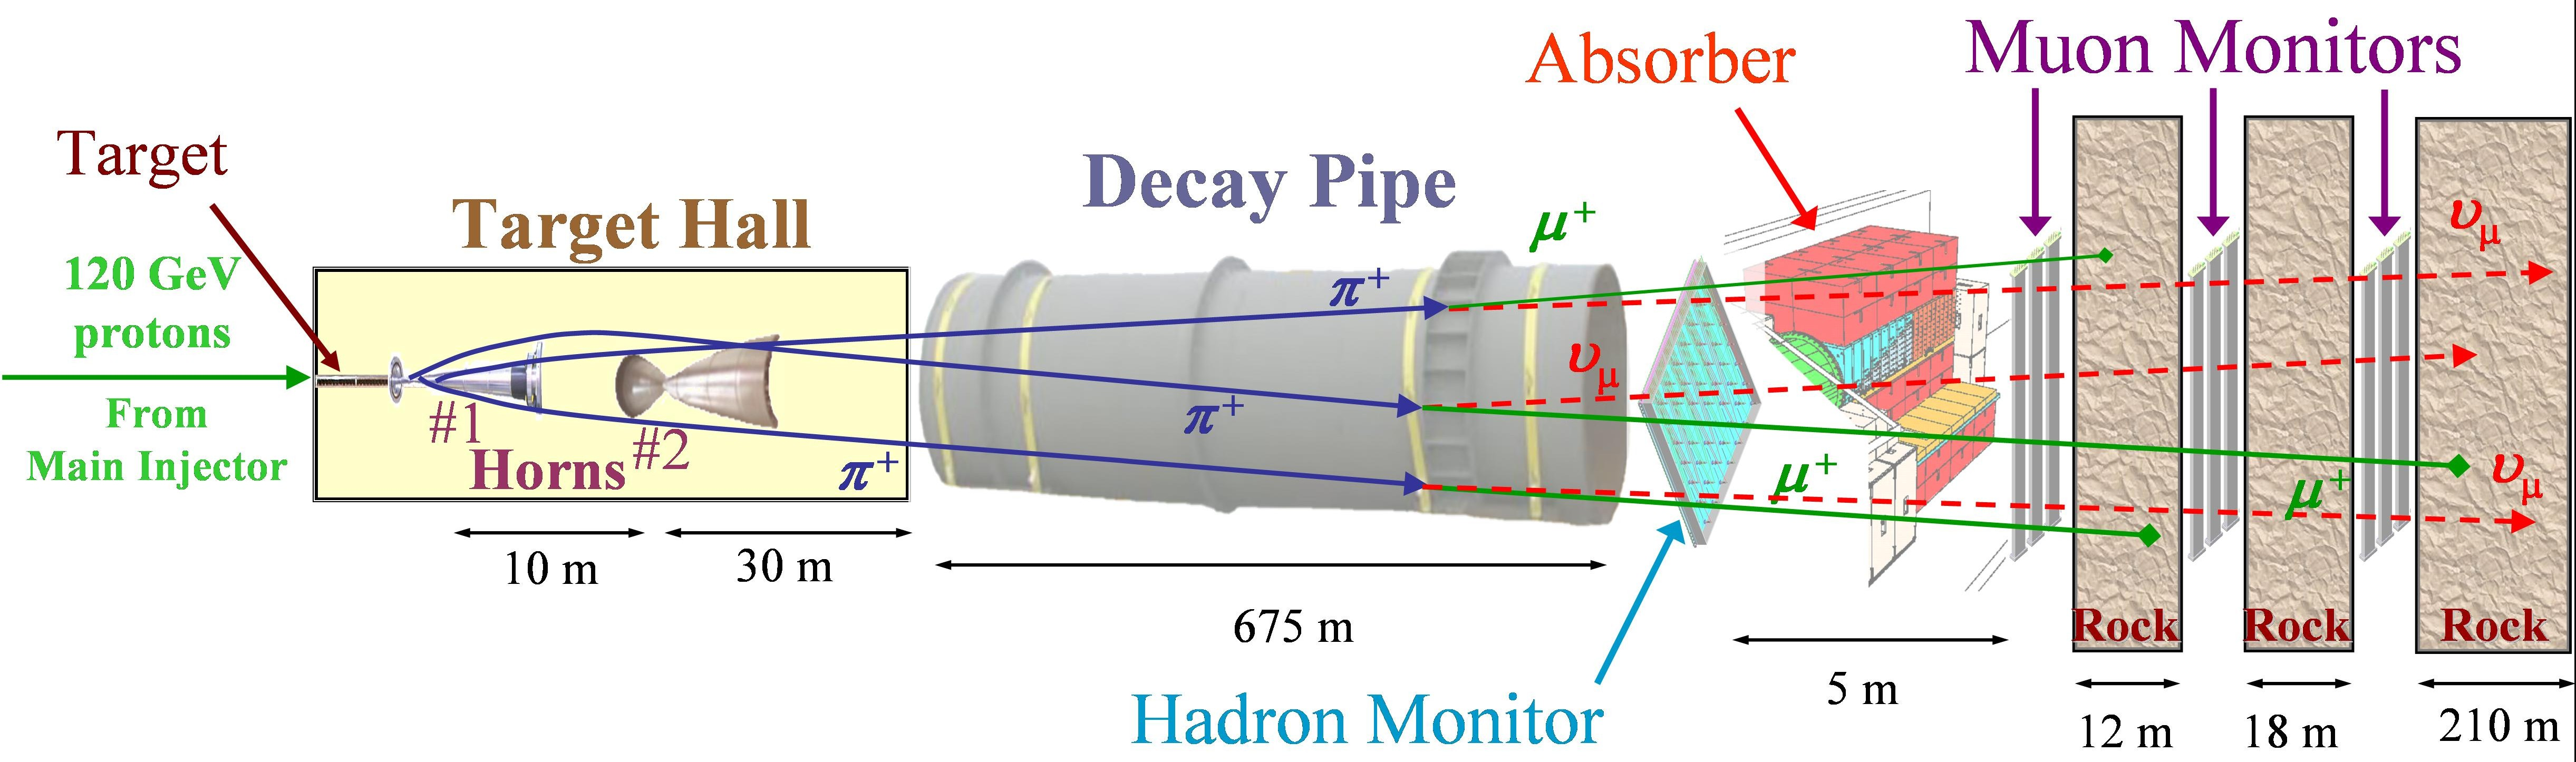
\includegraphics[width=\textwidth]{Plots/NOvAExperiment/BeamlineAlternative.jpg}
\caption[The schematic of the NuMI beam facility]{
The \acrshort{NuMI} neutrino beam starts on the left hand side with protons from the \acrshort{MI} impinged on a graphite target producing mainly pions and kaons. These are then focused and charge-selected by two focusing horns, after which they decay inside the decay pipe into a high-purity $\nu_\mu$ or $\overline{\nu}_\mu$ beam. The residual hadrons are stopped and monitored in the hadron absorber and the remaining muons are recorded with muon monitors and absorbed inside the rock. Figure from \cite{NuMI.pdf}.
%The schematic of the NuMI beam facility. The beam travels from left to right. The individual components shown are not to scale. Protons originate as $H^-$ ions, which are converted into protons in the Booster, sent to the main injector, where they are finally accelerated to $120\,\si{\giga\electronvolt}$, bent downward by $58\,\si{\milli\radian}$ and transported $350\,\si{\meter}$ to the $1.2\,\si{\meter}$ long NuMI target. The protons are incident on the graphite target and the produced hadrons are focused by two magnetic horns, located in about $40\,\si{\meter}$ long target hall, with about $19\,\si{\meter}$ separation between the two horns. Hadrons then enter a $675\,\si{\meter}$ long decay pipe made of steel, with $2\,\si{\meter}$ diameter, which serves as vacuum or low density environment for the mesons to propagate and decay into tertiary mesons, charged leptons and neutrinos. A hadron monitor is located at the end of the decay volume just in front of the $5\,\si{\meter}$ thick aluminium, steel and concrete absorber to record the profile of the residual hadrons. Of the particles interacting in the absorber, the principal component (approximately $80\%$) is the proton beam that has not interacted. The remainder are mainly mesons which have not decayed in the pipe or secondary protons. The absorber not only stops most of the particles still remaining in the beam but also acts as a shield against radiation. Muons and neutrinos deposit little or no energy in the absorber and continue into unexcavated rock with three muon monitors allowing measurement of the residual muon flux. The $240\,\si{\meter}$ of rock following the absorber stops the muons remaining in the beam but allows the neutrinos to pass\cite{numi}. 
}
\label{fig:NOvANuMI}
\end{figure}

The proton beam passes through a collimating baffle before hitting a $\sim\unit[1.2]{m}$-long (equal to about two interaction lengths) graphite target \cite{LEOFluxPredictionAtNuMI.pdf}, producing hadrons, predominantly pions and kaons \cite{NuMI.pdf}. These are then focused and selected by two parabolic magnetic `horns'. The focused hadrons pass through a $\unit[675]{m}$-long decay pipe filled with helium to create a low density environment for hadrons to propagate and decay in flight into either neutrinos or antineutrinos. High energy hadrons that do not decay in the decay pipe are absorbed within a massive aluminium, steel, and concrete hadron absorber and monitored with a hadron monitor. The leftover muons are ranged out in dolomite rock after the absorber and monitored using three muon monitors. The hadron and muon monitors are ionization chambers, used to monitor the quality, location and relative intensity of the beam.

Using a positive current inside the horns focuses positively charged particles, which then decay into neutrinos, and removes negatively charged particles. Reversing the horn current focuses negatively charged particles, which decay into antineutrinos, and defocuses positively charged particles. The neutrino mode is therefore called \gls{FHC} and the antineutrino mode is called \gls{RHC}. The composition of the neutrino beam for both these modes at the \gls{NOvA} \gls{ND} is shown in Fig.~\ref{fig:NOvABeamComponents}, displaying the very high purity of the $\nu_\mu$ or $\overline{\nu}_\mu$ component in the \gls{FHC} ro \gls{RHC} beam respectively \cite{NuMI.pdf}.

\begin{figure}[!htb]  
  \centering
  \includegraphics*[width=.495\textwidth]{Plots/NOvAExperiment/NuMIBeamComponentsNDFHC.pdf}
  \noindent\centering
  \includegraphics*[width=.495\textwidth]{Plots/NOvAExperiment/NuMIBeamComponentsNDRHC.pdf}
  \caption[NuMI neutrino beam components in the NOvA near detector]{The components of the neutrino beam at the \acrshort{NOvA} \acrshort{ND} per one \acrshort{NuMI} spill in the \acrshort{FHC} regime shown on the left and the \acrshort{RHC} regime on the right. The $\nu_\mu$ $\left(\overline{\nu}_\mu\right)$ composition in the \acrshort{FHC} (\acrshort{RHC}) regime is 93.8\% (92.5\%), with a wrong sign contribution of 5.3\% (6.6\%) and only 0.9\% (0.9\%) contamination by $\nu_e$ $\left(\overline{\nu}_e\right)$, showing the high purity of $\nu_\mu$ and $\overline{\nu}_\mu$ in the neutrino beam for \acrshort{NOvA}. Beam composition values calculated for neutrinos with energies between $\unit[1-5]{GeV}$. Figures are from internal \acrshort{NOvA} repository \cite{NOvA-doc-20843}.}
 \label{fig:NOvABeamComponents}
\end{figure}

The resulting neutrino beam energy distribution is peaked at $\sim\unit[7]{GeV}$ with a wide energy band. However, thanks to the kinematics of the dominant pion decay, by placing the \gls{NOvA} \gls{ND} and \gls{FD} $\unit[14.6]{mrad}$ ($\approx\unit[0.8]{\degree}$) off the main \gls{NuMI} beam axis, \gls{NOvA} achieves a narrow band neutrino flux peaked at $\unit[1.8]{GeV}$ \cite{NOvAResults2021.pdf,NOvATechreport.pdf}, as can be seen in Fig.~\ref{fig:NOvAOffAxis}. Using an off-axis neutrino flux increases the neutrino beam around $\unit[2]{GeV}$ about 5-fold compared to the on-axis flux and narrow-band peak enhances background rejection for the $\nu_e$ appearance analysis \cite{NOvATechreport.pdf}.

%Protons originate as $\textsc{H}^-$ ions, accelerated by the Linac to $\unit[400]{MeV}$, converted to protons and further accelerated to $\unit[8]{GeV}$ in the Booster, to be passed to the Main Injector which finally accelerates them to $\unit[120]{GeV}$ . Protons are then extracted, bent down to point towards the MINOS/NOvA Far Detector, and transported to the NuMI target \cite{NuMI.pdf}. The current beam power is $\sim\unit[700]{kW}$ with a plan \cite{PIP2.pdf} of reaching more than $\unit[1]{MW}$ beam power in the future upgrades.
%The NuMI target is a graphite fin, $\unit[7.4]{mm}$ wide, $\unit[63]{mm}$ tall and $\approx\unit[120]{cm}$ long (along the beam direction)\footnote{Previous target proportion were $\unit[6.4]{mm}$ W, $\unit[15]{mm}$ H and $\unit[95.38]{cm}$ L used in low energy design (see lower) \cite{NuMI.pdf}.} \cite{LEOFluxPredictionAtNuMI.pdf}. Protons interact in the target producing hadrons, predominantly pions and kaons \cite{NuMI.pdf}.

%The off-axis location means that both NOvA detectors are sited $14.6\,\si{\milli\radian}$ off the NuMI beam axis, in contrast to the MINOS Far Detector. This is because at around $14\,\si{\milli\radian}$, the energy of the neutrino does not have a strong dependence on the energy of the parent pion (fig. \ref{angleoff}), and also at this angle, the medium energy beam produces a narrow energy beam with approximately five times more neutrinos at $2\,\si{\giga\electronvolt}$ (fig. \ref{off-axis}), which is well-matched to the oscillation maximum expected to be at $1.6\,\si{\giga\electronvolt}$, thus maximizing the experiment’s neutrino oscillation sensitivity. In addition to the increased flux, the narrowness of the off-axis spectra enhances background rejection.\cite{techreport}

\begin{figure}[!htb]  
  \centering
  \includegraphics*[width=.48\textwidth]{Plots/NOvAExperiment/PionOffAxis.pdf}
  \noindent\centering
  \includegraphics*[width=.51\textwidth]{Plots/NOvAExperiment/OffAxisFluxPionEmbedded.pdf}
  \caption[The NOvA off-axis beam concept]{(Left) Dependence of the neutrino energy on the parent pion's energy and (right) neutrino energy distribution for an on-axis beam and three different off-axis beam designs. The case for \acrshort{NOvA} is shown in red and results in a narrow neutrino energy distribution around $\unit[2]{GeV}$, with limited dependence on the parent pion's energy. Figure from \cite{NOvATechreport.pdf}}
 \label{fig:NOvAOffAxis}
\end{figure}

\section{The NOvA detectors}\label{sec:NOvADetectors}

The two main \gls{NOvA} detectors are the \gls{ND}, located in \gls{Fermilab} $\sim\unit[1]{km}$ from the \gls{NuMI} target and $\sim\unit[100]{m}$ under ground, and the \gls{FD}, located $\sim\unit[810]{km}$ from \gls{Fermilab} at Ash River in north Minnesota, partially underground with a rock overburden \cite{NOvATechreport.pdf}. \gls{NOvA} also operated a detector prototype called \gls{NDOS}, which was used for early research and development of detector components and analysis \cite{NOvAStatusAndOutlook.pdf}. Additionally, \gls{NOvA} operated a Test Beam detector, described in detail in Sec.~\ref{sec:TBExperiment}. The scales of the \gls{ND} and \gls{FD} are shown in Fig.~\ref{fig:NOvADetectors}.

%The FD has an approximately 130kHz of cosmics

\begin{figure}[ht]
\centering
%is pdf-a
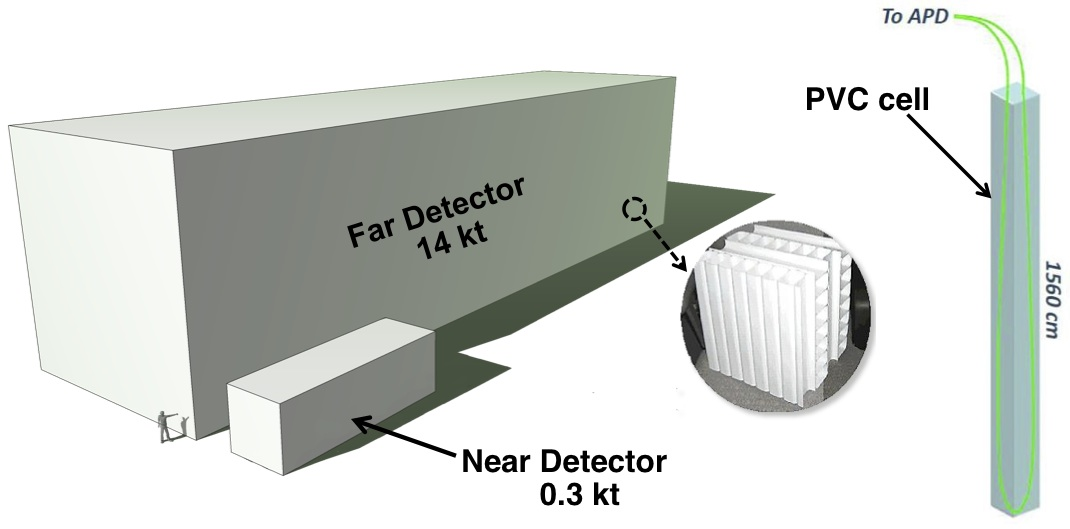
\includegraphics[width=1\textwidth]{Plots/NOvAExperiment/NOvADetectors.png}
\caption[NOvA detectors]{Schematic description of the scale and composition of the \acrshort{NOvA} \gls{ND} and \gls{FD}. The inset shows a photo of the orthogonal planes made out of \acrshort{PVC} cells. An example of a \acrshort{FD} cell containing liquid scintillator and a looped \acrshort{WLS} fibre attached to an \acrshort{APD} is shown on the right \cite{NeutrinoDetectorsForOscExp.pdf}.}
\label{fig:NOvADetectors}
\end{figure}

All \gls{NOvA} detectors are highly segmented, highly active, functionally identical tracking calorimeters made up of \gls{PVC} cells filled with liquid scintillator. Each cell is a long rectangular cuboid with depth of $\unit[5.9]{cm}$ and width of $\unit[3.8]{cm}$ (with some variations), with cell length extending to the full width/height of each detector, which is $\sim\unit[4.1]{m}$ for the \gls{ND} and $\sim\unit[15.6]{m}$ for the \gls{FD} \cite{NOvATechreport.pdf}. An example of a \gls{FD} cell is shown on the right of Fig.~\ref{fig:NOvADetectors}.

Cells are connected side-by-side into a 16 cell-wide extrusions with $\unit[3.3]{mm}$-wide walls between cells and $\unit[4.9]{mm}$-wide walls on the outsides of the extrusions. The first and last cell of each extrusion are $\sim\unit[3]{mm}$ narrower than the rest of the cells. Two extrusions are connected side-by-side to form a 32 cell-wide module, with each module having a separate readout (see Sec.~\ref{sec:DAQ}). In the \gls{FD}, 12 modules are connected side-by-side to form one plane of the detector. In the \gls{ND} only 3 modules make up a plane. Planes are positioned one after another, alternating between vertical and horizontal orientation, and grouped into diblocks, each containing 64 planes. The \gls{FD} contains 14 diblocks, totalling 896 planes, whereas the \gls{ND} contains 3 diblocks totalling 192 planes. The \gls{ND} also contains a Muon Catcher region, positioned right after the active region, consisting of 22 planes of the normal \gls{NOvA} detector design, 2 modules high and 3 modules wide, sandwiched with 10 steel plates to help range out muons mainly from the $\nu_\mu$ charged current interactions~\cite{NOvAStatusAndOutlook.pdf,NOvATechreport.pdf}.

The \gls{NOvA} coordinate system is centred with $\left(0,0,0\right)$ in the centre of the first plane, relative to the beam direction. The x axis runs from left to right when facing the detector, y axis from bottom to top and z axis runs perpendicular to the planes along the beam direction.

Each cell is filled with a liquid scintillator consisting of mineral oil with $4.1\%$ pseudocumene as the scintillant \cite{NOvAScintillators.pdf}. Each cell contains a single wavelength shifting fibre with double the length of the cell, looping at one end and connecting to the readout at the other. The \gls{PVC} walls of the cells are loaded with highly reflective titanium dioxide, with light typically bouncing off the \gls{PVC} walls $\sim8$ times before being captured by the \gls{WLS} fibre \cite{NOvATechreport.pdf}.
%As light travels through the fibre, it is attenuated by about a fraction of ten for the \gls{FD} cells \todo{Figure out what is the correct statement here}. 

The final dimensions of the \gls{FD} are $\unit[15.6]{m}\times\unit[15.6]{m}\times\unit[60]{m}$ with a total mass of $\unit[14]{kT}$ and for the \gls{ND} the dimensions are $\unit[3.8]{m}\times\unit[3.8]{m}\times\unit[12.8]{m}$ with a mass of about $\unit[0.3]{kT}$ \cite{NOvAHalfTimeOverview2022.pdf}. The active volume, consisting only of the liquid scintillator without the \gls{PVC} structure, makes up about $70\%$ of the total detector volume \cite{NOvATechreport.pdf}.

The \gls{NOvA} detectors are specifically designed for electromagnetic shower identification, with a radiation length of $\unit[38]{cm}$, which amounts to $\sim 7$ planes for particles travelling perpendicular to the detector planes \cite{NOvAStatusAndOutlook.pdf}. This is particularly useful to distinguish electrons from $\pi^0$s.

We can calculate the minimum energy an electron needs to have to cross one cell ($\unit[5.9]{cm}$) of the \gls{NOvA} detector by using the measured scintillator density $\unit[0.86]{g/cm^3}$ \cite{NOvA-doc-11886}, which gives us the required range of $\sim\unit[5]{g/cm^2}$. Comparing this to measured values for the electron range \cite{NISTParticleRangeTables} in the continuous slowing down approximation in a Polyethylene (approximation of the \gls{NOvA} scintillator \cite{NOvA-doc-13579-FACalorimetricEnergyScale}), gives us an estimate of the lowest detectable electron energy as $E_{e}\gtrsim\unit[10]{MeV}$.
%We can calculate what is the minimum energy for any particle to be recorded in the \gls{NOvA} detector, by taking the density of \gls{NOvA} liquid scintillator as $\unit[0.86]{g/cm^3}$ \cite{NOvA-doc-11886} and looking up the particle range in the continuous slowing down approximation and approximating the liquid scintillator as polyethylene \cite{NOvA-doc-13579-FACalorimetricEnergyScale}. We take the depth of one \gls{NOvA} cell ($\unit[5.9]{cm}$) as the minimum distance particle needs to travel to be recorded in the \gls{NOvA} detector. For electrons we get that the minimum energy an electron needs to have to be recorded in \gls{NOvA} is $\sim\unit[15]{MeV}$ \cite{NISTParticleRangeTables}. 
%The MIP energy loss for electrons (similarly to muons) can be found with a similar method as used in the AbsCal\_technote\_1stAna in TestBeam (page 2)

\section{Readout and data acquisition}\label{sec:DAQ}

The signal from the \gls{WLS} fibres is read out by an \gls{APD}, converting the scintillation light into electrical signal, with a high quantum efficiency of $\sim 85\%$ and a gain of $100$ \cite{NOvATechreport.pdf}. An example \gls{APD} is shown in Fig.~\ref{fig:NOvAAPD}. Both ends of each fibre correspond to a single readout channel and are connected to one of the 32 pixels on the \gls{APD}, organized in four rows of 8 pixels, with each \gls{APD} reading out signal from one module. To maximise the signal to noise ratio, the \glspl{APD} are cooled to $\unit[-15]{\degree C}$ by a thermoelectric cooler, with heat carried away by a water cooling system.

The combination of the \gls{APD} quantum efficiency and the light yield, determined by the \gls{PVC} reflectivity and the scintillator and \gls{WLS} fibre responses, result in a signal requirement of at least 20 \gls{PE} in response to minimum ionizing radiation at the far end of the \gls{FD} cell.

%TDR-12.2.1:"NOvA readout electronics requires, at minimum, a 20 photoelectron signal in response to minimum ionizing radiation at the far-end of a 15.5 m NOvA cell as discussed in Chapter 6. The signal strength is due to the APD quantum efficiency and the light yield in response to ionizing radiation. The light yield, in turn, is due to a combination of the PVC reflectivity, the scintillator and wavelength-shifting fiber responses."

%For some reason the TDR I have downloaded doesn't have the full chapter 14. Full TDR can be found in docdb:2678 chapter by chapter.

\begin{figure}[!htb]  
  \centering
  \includegraphics*[width=.495\textwidth]{Plots/NOvAExperiment/NOvAAPDMountedWithLabels.jpg}
  \noindent\centering
  \includegraphics*[width=.495\textwidth]{Plots/NOvAExperiment/NOvAAPDBottomWithLabels.jpg}
  \caption[NOvA Avalanche Photo Diods]{The modules with \acrshort{APD}s for \acrshort{NOvA} mounted on top of the detector on the left picture, and shown from the bottom on the right. The individual components of the module are described. The left picture shows a disconnected ribbon cable and ground cable, which are normally connected to the front end board.}
 \label{fig:NOvAAPD}
\end{figure}

Each \gls{APD} is connected to a single \gls{FEB}, shown in Fig.~\ref{fig:NOvAFEB}. The \gls{FEB} amplifies and integrates the \gls{APD} signal, determines its amplitude and arrival time, before passing it to the \gls{DAQ} system. On the \gls{FEB} the \gls{APD} signal is first passed to a custom \gls{NOvA} \gls{ASIC}, which is designed to maximize the detector sensitivity to small signals. \glspl{ASIC} amplify, shape and combine the signal, before sending it to an \gls{ADC}. The combined noise from the \gls{APD} and the amplifier is equivalent to about 4 \glspl{PE}, which, compared to an average \gls{PE} yield from the far end of the \gls{FD} cell of 30, results in a good signal and noise separation \cite{NOvATechreport.pdf}. The digitized data from an \gls{ADC} is sent to a \gls{FPGA}, which extracts the time and amplitude of the \gls{ADC} signals, while subtracting noise based on a settable threshold. The \glspl{FPGA} employ multiple correlated sampling methods to reduce noise and improve time resolution of the signal \cite{NOvADAQ.pdf}.

\begin{figure}[!htb]  
  \centering
  \includegraphics*[width=\textwidth]{Plots/NOvAExperiment/NOvAFEBWithLabels.jpg}
  \caption[NOvA Front End Board]{An example of a \acrshort{NOvA} \acrshort{FEB} with individual components labelled.}
 \label{fig:NOvAFEB}
\end{figure}

%TDR:Major components are the carrier board connector location at the left, which brings the APD signals to the NOvA ASIC, which performs integration, shaping, and multiplexing. The chip immediately to the right is the ADC to digitize the signals, and FPGA for control, signal processing, and communication. Data from the ADC is sent to an FPGA where multiple correlated sampling is used to remove low frequency noise. This type of Digital Signal Processing (DSP) also reduces the noise level and increases the time resolution.

All of the \gls{NOvA} front end electronics (\glspl{APD} and \glspl{FEB}) are operated in a continuous readout mode, without requiring any external triggers \cite{NOvATechreport.pdf}. Due to higher detector activity during beam spills, the \gls{ND} \glspl{FEB} work at a higher frequency of $\unit[8]{MHz}$, whereas the \gls{FD} \glspl{FEB} suffice with $\unit[2]{MHz}$ sampling frequency \cite{NOvADAQ.pdf}.

Data from up to 64 \glspl{FEB} are concentrated in a \gls{DCM}, which concatenates and packages the data into $\unit[5]{ms}$ time slices, before sending it to the buffer nodes. \glspl{DCM} are also connected to the timing system and pass a single unified timing measurement to the \glspl{FEB} to maintain synchronization across the detector~\cite{NOvADAQ.pdf}.
%The timing information is calibration off-line to account for differences between fibre and cable distances and to achieve a superb timing resolution \cite{NinerThesis} - I don't think I need to talk about the timing calibration here tbh. The NOvA calibration process technically also involves \textbf{timing calibration}, which corrects for the time differences of the signal to be processed \cite{NinerThesis}.

The buffer nodes cache the data for at least 20 seconds while receiving information from the trigger system. Each trigger uses a time window based either on the time of the \gls{NuMI} beam spill, on a periodic interval for monitoring and for the readout of cosmic events, or on one of the activity-based data-driven triggers \cite{NOvADAQ.pdf}. Data that fall within any of the trigger windows are sent to a data logger system, where they are merged to form events, before being written to files for offline processing and sent to an online monitoring system. Files are organized based on a unique combination of run and subrun numbers, with runs corresponding to data taking periods with constant detector conditions and limited to either 64 subruns or 24 hours. Subruns are delineated either by a $\unit[2]{GB}$ file size constraint or a 1-hour timeout limit \cite{NOvA-doc-13546}.

The detectors are continuously monitored to ensure data stability and quality. Subruns with suboptimal detector conditions or with events failing basic quality criteria are flagged as `bad' and recorded in a `bad runs list' \cite{NOvA-doc-13546}. Additionally, individual readout channel are assessed on a per-subrun basis, with those with too high or too low hit rates marked as `bad' \cite{NOvA-doc-12771}. Both the `good runs' list and the `bad channel' maps are used to inform event processing and during simulation to emulate real detector conditions.

%Data for calibration and non-beam physics channels is collected and a variety of data-driven triggers using real-time reconstruction algorithms run on data stored in an online buffer farm at each detector [26].  Beam events are collected in both detectors using a 550 μs time window centered on the 10 μs beam spill window, triggered by a signal derived from the accelerator controls system. The wide time window of data collection compared to the beam spill is used to sample cosmic-ray activity and noise under the precise detector conditions that apply to the beam data. [NOvAHalfTimeOverview2022.pdf]

%Maybe I should write here what is the event rate?

%Maybe write about what information do we have about each event at this stage: timing, peak ADC, cell, plane, run, subrun. Grouped into triggered windows?
% "the time, location, and pulseheight of those signals are recorded as a hit" [NOvAHalfTimeOverview2022.pdf]

\section{Simulation}\label{sec:NOvASimulation}
To extract neutrino oscillation parameters, or to test a hypothesis, \gls{NOvA} uses a series of simulations to make predictions according to various physical models \cite{NOvASimulationOld-Fluka.pdf}.
%To simulation the expected signal from the NOvA detectors,
%To get a prediction of any possible signal events or their background in the NOvA detectors,
% we use a series of simulations, tuned or corrected by both internal and external measurements to better match the current state of the art knowledge \cite{NOvASimulationOld-Fluka.pdf}.
The simulation chain can be divided into four parts: simulation of the neutrino beam, simulation of neutrino interactions within the \gls{NOvA} detectors, simulation of cosmic particles interacting in the \gls{NOvA} detector and simulation of the detector and readout response.

To simulate the neutrino beam, \gls{NOvA} uses a simulation based on the \texttt{GEANT4} v9.2.p03~\cite{GEANT4.pdf} \gls{MC} event generator with a detailed model of the \gls{NuMI} beamline \cite{ZPavlovicThesisG4NuMI_2008.pdf}, as described in Sec.~\ref{sec:NuMI}. The simulation starts with the $\unit[120]{GeV/c}$ \gls{MI} protons interacting within the long carbon target and producing hadrons, mainly $\pi, K$ and secondary protons. This is followed by transport and possible further interaction of hadrons within the focusing system, until finally ending with hadron decays producing the neutrino beam.

To account for the inherently imprecise theoretical models used in GEANT4, \gls{NOvA} uses the \gls{PPFX} to incorporate external measurements of yields and cross sections of hadron interactions inside the target and the other \gls{NuMI} materials into the neutrino beam prediction~\cite{NuMIFlux.pdf}. The current version of \gls{PPFX} is limited by the results available during its creation and only corrects the most frequent interactions while assigning conservative systematic uncertainties to the rest (see Sec.~\ref{sec:NOvASystematics}).
%Furthermore, the available data were measured with specific incident energies, often different from the $\unit[120]{GeV}$ of the \gls{NuMI} protons, and have to be scaled using an additional \gls{MC} generator called FLUKA \cite{FLUKA_01,FLUKA_02}.
For the most common $\pi, K$ and $p$ production, \gls{PPFX} uses the NA49 measurements \cite{NA49:Inclusive_production_of_charged_pions.pdf, NA49DataKaons.pdf, NA49pc-proton2013.pdf} of $\unit[158]{GeV/c}$ protons interacting on a thin (few percent of interaction length) carbon target. To expand the kinematic coverage, \gls{PPFX} uses a few data points from Barton et al~\cite{BartonHadProd1983.pdf} for the $\pi$ production and $K/\pi$ ratios from the \gls{MIPP} \cite{pionToKaonIn_pC.pdf} experiment for the production of $K$. These results have to be scaled to the $\unit[20-120]{GeV/c}$ incident proton moment seen throughout \gls{NuMI} using the FLUKA \cite{FLUKA_01,FLUKA_02} \gls{MC} generator.

%For the $K$ production from $p+C$ interaction, important for higher neutrino energies and electron neutrinos, \gls{PPFX} uses the NA49 $K$ data \cite{NA49DataKaons.pdf} together with the NA49 $\pi$ data \cite{NA49:Inclusive_production_of_charged_pions.pdf} multiplied by the $K/\pi$ ratios of yields on thin carbon target from the MIPP experiment \cite{pionToKaonIn_pC.pdf}. Lastly, for the nucleon production, \gls{PPFX} uses the NA49 data on \gls{QE} interactions \cite{NA49pc-proton2013.pdf}. All the other interactions inside \gls{NuMI}, such as interaction in non-carbon targets, or interactions with hadrons other than protons, are either extrapolated from the previously mentioned measurements, or are not corrected for and a significant systematic uncertainty is assigned to them \cite{NuMIFlux.pdf}.

%For the most common $\pi$ production, \gls{PPFX} uses the NA49 measurements \cite{NA49:Inclusive_production_of_charged_pions.pdf} of $\unit[158]{GeV/c}$ protons interacting on a thin (few percent of interaction length) carbon target, with a few data points from Barton et al~\cite{BartonHadProd1983.pdf} to expand the kinematic coverage. These then have to be scaled to the $\unit[20-120]{GeV/c}$ incident proton energies seen in \gls{NOvA} using the FLUKA \cite{FLUKA_01,FLUKA_02} \gls{MC} generator. For the $K$ production from $p+C$ interaction, important for higher neutrino energies and electron neutrinos, \gls{PPFX} uses the NA49 $K$ data \cite{NA49DataKaons.pdf} together with the NA49 $\pi$ data \cite{NA49:Inclusive_production_of_charged_pions.pdf} multiplied by the $K/\pi$ ratios of yields on thin carbon target from the MIPP experiment \cite{pionToKaonIn_pC.pdf}. Lastly, for the nucleon production, \gls{PPFX} uses the NA49 data on \gls{QE} interactions \cite{NA49pc-proton2013.pdf}. All the other interactions inside \gls{NuMI}, such as interaction in non-carbon targets, or interactions with hadrons other than protons, are either extrapolated from the previously mentioned measurements, or are not corrected for and a significant systematic uncertainty is assigned to them \cite{NuMIFlux.pdf}.\todo{How significant is the uncertainty?}

There are two new experiments that measure the production and interaction of hadrons on various targets and incident energies, specifically designed to improve the prediction of neutrino beams.
The most impactful measurements from the NA61 experiment are of the $\unit[120]{GeV/c}$ protons on a thin carbon target \cite{2019_NA61_ProdAndInelXSec_protonOnDiffTargets60And120GeV._results.pdf, NA61_hadprodFrompC_120GeV_2023.pdf, NA61_ResonanceProdFrompC_120GeV_2023.pdf}, of the hadron incident interactions on various materials \cite{2019_had_prod_at_Pi_on_C_and_Be.pdf}, and of the $\unit[120]{GeV/c}$ protons on a \gls{NuMI} replica target \cite{ThickTargetLimit.pdf}. Additionally, the \gls{Fermilab}-based EMPHATIC experiment~\cite{EMPHATICProposal2019.pdf} is currently analysing a broad range of hadron production and secondary and tertiary interaction measurements for neutrino beam prediction with a significant involvement of \gls{NOvA} and \gls{DUNE} collaborators. Inclusion of the results from both of these measurement is currently under way and will significantly improve the neutrino beam prediction in \gls{NOvA} \cite{ThickTargetLimit.pdf}.

%I worked on implementing data from the NA61 experiment on hadron production from $p+C$ interaction on a thin carbon target at $\unit[31]{GeV/c}$~\cite{2015_hadron_prod_pC_2009data.pdf}, motivated by possible reduction in the $K$ production systematic uncertainty. This work is still ongoing and will be implemented into \gls{PPFX} and \gls{NOvA} together with the rest of the NA61 measurement. The most impactful measurement will be of the hadron production from $p+C$ interaction on a thin carbon target at $\unit[120]{GeV/c}$  (no energy scaling required), measurements of $p+C$ and $p+Be$ at different incident energies \cite{2019_NA61_ProdAndInelXSec_protonOnDiffTargets60And120GeV._results.pdf}, $\pi+C$ and $\pi+Be$ measurements at $\unit[60]{GeV/c}$~\cite{2019_had_prod_at_Pi_on_C_and_Be.pdf}, resonance production measurements from $\unit[120]{GeV/C}$ $p+C$ \cite{NA61_ResonanceProdFrompC_120GeV_2023.pdf}, and probably the most impactful one, the yet unpublished measurement of hadron production yield on a \gls{NOvA}-era \gls{NuMI} replica target at $\unit[120]{GeV/c}$ \cite{ThickTargetLimit.pdf}. NA61 also measured the hadron production yield for the \gls{T2K} experiment's replica target \cite{2019_hadron_yields_T2K_replica.pdf}, which significantly reduced the neutrino flux systematic uncertainty for the \gls{T2K} measurements \cite{ThickTargetLimit.pdf}. The second experiment is EMPHATIC~\cite{EMPHATICProposal2019.pdf}, which is currently analysing a broad range of hadron production measurements, mainly the secondary and tertiary interactions of various projectiles with a wide range of incident energies and thin target materials, complementary to the NA61 measurements.

%From NOvAResults2021.pdf: The neutrino flux delivered to the detectors is calculated using GEANT4-based simulations of particle production and transport through the beamline components [NuMI.pdf,GEANT4.pdf] reweighted to incorporate external measurements using the package to predict the flux (PPFX) [NuMIFlux.pdf,30–48].

%From NOvAResultsCombinedNuAnu2019.pdf: The flux of neutrinos delivered to the detectors is calculated using a simulation of the production and transport of particles through the beamline components [22,25] reweighted to incorporate external measurements [26–45].

%From NOvAHalfTimeOverview2022.pdf: Neutrino interactions in NOvA are simulated with a chain of software packages. The neutrino flux is modeled using G4NuMI, a geant based description of the NuMI beam line [Z. Pavlovic thesis]. The raw flux from G4NuMI is then modified using the PPFX package to better match the products of the interactions in the extended target to the world’s hadron production data [NuMIFlux.pdf].

%%%%%%%%%%%%%%%%%%%%%%%%%%%%%%%%%%%%%%%%%%%%%%%%%%%%%%%%%%%%%%%%%%%%%%%%%%%%%%%
%%%% Master's thesis on flux simulation
\iffalse
There are often multiple interactions within the target and in the materials downstream of it and since the hadron production process is governed by non-perturbative QCD and occurs in the nucleus, highly accurate theoretical predictions are not possible \cite{NuMIFlux.pdf,LEOFluxPredictionAtNuMI.pdf}. NOvA therefore tunes and corrects possible mismodeling of the model using external data in a package developed for MINERvA experiment called Package to Predict the Flux (PPFX) \cite{LEOFluxPredictionAtNuMI.pdf}.

%...Those models are not necessarily accurate but can be tuned or benchmarked by comparing their predictions to measurements of hadron production. Recent measurements of pion production on a thick (two interaction length) carbon target have been released by MIPP [4], and measurements of pion production on a thin (few per cent interaction length) carbon target are available from NA49 [5]. In addition, there are several other hadron production measurements on various materials, using both proton and pion beams, that can be used to constrain a neutrino beamline simulation.[NuMIFlux.pdf]

%Roughly 85% of the interactions that produce particles that lead to muon neutrinos passing through MINERvA are from protons interacting on carbon. Other relevant materials are aluminum (horns), iron (decay pipe walls), helium (decay pipe gas), and air (target hall). Interactions of π ± , K ± and n created in the initial proton interaction, or subsequent interactions, are subdominant but non-negligible. When protons collide with carbon, the interactions can produce pions, kaons, neutrons, strange baryons, and lower energy protons. These particles, if they do not decay first, can interact either in the target or in other downstream material to create tertiary particles that can also decay into neutrinos. \cite{NuMIFlux.pdf}

PPFX is used to correct each interaction of neutrino's ancestry chain by weighting it with a factor computed from external experimental measurements of yields or invariant differential cross-sections \cite{LEOFluxPredictionAtNuMI.pdf}

The kinematic values of the initial particles (like the initial $\unit[120]{GeV}$ proton interacting on carbon in NuMI) are not always the same between the measured interaction and the required values. To solve this we use the \textit{Feynman-x} ($x_{F}$) scaling variable. Feynman speculated \cite{feynman1969.pdf} that expressing the cross-sections of inclusive high energy hadronic collisions in terms of $x_{F}$ would make the cross-section scaling energy independent \cite{LEOFluxPredictionAtNuMI.pdf}.
%$c_i$ is the \textit{central value} of the weight

There are two main experiments whose results are used in the PPFX. NA49 \cite{NA49:Inclusive_production_of_charged_pions.pdf}, which used $\unit[158]{GeV}$ protons interacting on carbon thin target, and MIPP \cite{pionToKaonIn_pC.pdf} which used protons from the Main Injector and both thin carbon target and the low energy NuMI target (thick target) \cite{PPFXTechnote2017.pdf}. Energy scaling of the external data to calculate the PPFX weight is performed by FLUKA\cite{NuMIFlux.pdf}

%%% Hadron production datasets:
%There are two major datasets available to constrain the process where protons interact on carbon and produce charged pions. One measurement, from NA49 [5], uses a thin target with an incident proton momentum of 158 GeV/c. The other measurement, from MIPP [4], uses an actual NuMI LE target and 120 GeV/c protons. These two datasets will be used to make separate “thin target” and “thick target” flux predictions by weighting each interaction leading to a neutrino going through MINERvA. We also use additional datasets to constrain kaon and nucleon production, and the absorption of particles in beamline materials. Where multiple interactions are constrained with data, the overall weight applied to the neutrino event is simply the product of the weights for each interaction.\cite{NuMIFlux.pdf}

For kaons with $x_{F}<0.2$ PPFX uses weights based on NA49 measurements\cite{NA49DataKaons.pdf} and for kaons with $0.2<x_{F}<0.5$ PPFX uses the $K/\pi$ yield ratio from the MIPP thin target measurements\cite{pionToKaonIn_pC.pdf} multiplied by NA49 thin target yields.
\fi
%%% End of master's on flux simulation
%%%%%%%%%%%%%%%%%%%%%%%%%%%%%%%%%%%%%%%%%%%%%%%%%%%%%%%%%%%%%%%%%%%%%%%%%%%%%%%

%Good description of PPFX, beam transport and the principal components is in the NOvA-T2K technote for Flux (doc-db:54582) https://nova-docdb.fnal.gov/cgi-bin/sso/ShowDocument?docid=54582

The output of the neutrino beam simulation is passed to the simulation of neutrino interactions inside the detectors, which is done with the GENIE v3.0.6~\cite{GENIE.pdf} neutrino \gls{MC} generator. GENIE allows users to choose the particular models for different types of neutrino interactions and particle propagation within the nucleus, as well as possible tunes to external measurements. The four main interaction modes in GENIE are the \gls{QE} \gls{CC} scattering, the \gls{Res}, the \gls{DIS}, and the \gls{COHpi} production. The special case of the \gls{2p2h} interaction via \gls{MEC} and the \gls{FSI} inside a nucleus are also considered. The initial state of the nucleus is represented by a local Fermi gas in the \gls{QE} and {2p2h} models, while a global relativistic Fermi gas is used for all other processes. Additionally, \gls{NOvA} adds a costume tune to the \gls{NOvA} $\nu_\mu$\gls{CC} data for a better constraint of the \gls{CC}\gls{MEC} interactions. \gls{NOvA} also uses a set of external $\pi$ interaction measurements to constrain the \gls{FSI} model. Table~\ref{tab:NuIntSimulationModels} shows the list of models and tunes for different interaction modes in \gls{NOvA} \cite{NOvAResults2021.pdf}.
% All of these are set by the \gls{CMC}, which is currently \texttt{N1810j0000} for \gls{NOvA}. 

\begin{table}[!ht]
\centering
%\def\arraystretch{1.4}
\caption{Models and tunes used in the NOvA simulation of neutrino interactions.}
\begin{tabular}{|l|l|l|}
\hline
Interaction & Model                  & Tune\\\hline
\gls{CC}\gls{QE} & Val\`{e}ncia \cite{ValenciaModel_NOvACCQE_2004.pdf} & External $\nu-\textsf{D}$ data \cite{NuDeuteriumScattering_NOvACCQETune_2016.pdf}\\
\gls{CC}\gls{MEC} & Val\`{e}ncia \cite{ValenciaModel_NOvACCQEMEC_2011.pdf,ValenciaModel_NOvAMEC_2013.pdf} & \gls{NOvA} $\nu_\mu$\gls{CC} data\\
\gls{Res} \& \gls{COHpi} & Berger-Sehgal \cite{BergerSehgal_ResonancePionProd_2007.pdf,BergerSehgalModel_CohPionProd_2009.pdf}          & External $\nu-A$ data\\
\gls{DIS} & Bodek-Yang \cite{BodekYangModel_NOvADIS_2003.pdf,HadronizationModelForNuDIS_NOvADIS_1988.pdf}            & External $\nu-A$ data\\
\gls{FSI} & Semi-classical cascade \cite{FSIModel_hNSemiClassicalCascade_1988.pdf} & External $\pi-^{12}\textsf{C}$ data\\\hline
\end{tabular}
\label{tab:NuIntSimulationModels}
\end{table}

%NOvANuMuCCPi0XSecMeasurement2023.pdf: Neutrino interactions are simulated with GENIE [17] v2.10.2. The GENIE simulation generates interactions via its four default production processes: quasielastic scattering, resonant baryon production, deep-inelastic scattering, and coherent pion production. Particles created via these primary processes are subsequently propagated though the nuclear medium using GENIE’s hA effective cascade FSI model [18,19].

% Describe that GENIE is highly costumizable and you can set up any generators you like. Ideally describe what parts are purely theoretical and what parts are tuned to external data. Also mention that NOvA is doing an internal tune to some of the parameters.

%From NOvAResults2021.pdf: Neutrino interactions are simulated using a custom model configuration of GENIE 3.0.6 [49,50] tuned to external and NOvA ND data.
%In this configuration, charged-current (CC) quasielastic (QE) scattering is simulated using the model of Nieves et al. [53], which includes the effects of long-range nucleon correlations calculated according to the random phase approximation (RPA) [53–55]. The CCQE axial vector form factor is a z-expansion parametrization tuned to neutrino-deuterium scattering data [56].
%CC interactions with two nucleons producing two holes (2p2h) are given by the IFIC València model [57,58]. The initial nuclear state is represented by a local Fermi gas in both the QE and 2p2h models, and by a global relativistic Fermi gas for all other processes.
%Baryon resonance (RES) and coherent pion production are simulated using the Berger-Sehgal models with final-state mass effects taken into account [59,60].
%Deep inelastic scattering (DIS) and nonresonant background below the DIS region are described using the Bodek-Yang model [61] with hadronization simulated by a data-driven parameterization [62] coupled to PYTHIA [63].
%Bare nucleon cross sections for RES, DIS, and nonresonant background processes are tuned by GENIE to neutrino scattering data.
%Final-state interactions (FSI) are simulated by the GENIE hN semi-classical intranuclear cascade model in which pion interaction probabilities are assigned according to Oset et al. [64] and pion-nucleon scattering data.

%The 2p2h and FSI models in this GENIE configuration are adjusted to produce a NOvA-specific neutrino interaction model tune. The 2p2h model is fit to $\nu_\mu$CC inclusive scattering data from the NOvA ND. Inspired by Gran et al. [65], this 2p2h tune enhances the base model as a function of energy and momentum transfer to the nucleus and is applied to all CC 2p2h interactions for both the neutrino and antineutrino beams. 
%The parameters governing $\pi^\pm$ and $\pi^0$ FSI are adjusted to obtain agreement with $\pi^+$ on $^{12}\textsf{C}$ scattering data [66–72].

%From NOvAResultsCombinedNuAnu2019.pdf: Neutrino interactions in the detector are simulated using GENIE [46] tuned to improve agreement with external measurements and ND data, reducing uncertainties in the extrapolation of measurements in the ND to the FD. As in Ref. [21], we set MA in the quasielastic dipole form factor to 1.04 GeV/c2 [47] and use corrections to the charged-current (CC) quasielastic cross section derived from the random phase approximation [48,49]. In this analysis, we also apply this effect to baryon resonances as a placeholder for the unknown nuclear effect that suppresses rates at a low four-momentum transfer in our and other measurements [50–53]. Additionally, we increase the rate of deep-inelastic scattering with hadronic mass W > 1.7 GeV/c2 by 10\% to match our observed counts of short track-length $\nu_\mu$CC events. We model multinucleon ejection interactions following Ref. [54] and adjust the rates in bins of energy transfer, $q_0$, and three-momentum transfer, $\left|\overrightarrow{q}\right|$, for $\nu_\mu$ and $\overline{\nu}_\mu$ separately to maximize agreement in the ND. The calculation of the $\nu_e$ and $\overline{\nu}_e$ rates uses these same models.

%From NOvAHalfTimeOverview2022.pdf: Neutrino interactions and final state interactions are modeled using the GENIE neutrino interaction generator [31]

%From master thesis: From there GENIE event generator \cite{GENIE.pdf} simulates neutrino interactions in the detector \cite{2019NOvAFHCRHCResults.pdf} and another GEANT4 simulates the detector response \cite{NOvASimulationOld-Fluka.pdf}. NOvA also tunes the cross-section model of the GENIE simulation to the ND data to reduce uncertainties in the extrapolation of measurements on the ND to the FD \cite{2019NOvAFHCRHCResults.pdf}.

Since the \gls{FD} is on the surface \gls{NOvA} also uses a simulation of cosmic rays generated with the \gls{MC} \gls{CRY} \cite{CRY}. The simulated cosmic muons are also used to calibrate \gls{NOvA} detectors \cite{NuMIFlux.pdf}. 

Particles that are created from neutrino interactions and cosmic rays are propagated through the \gls{NOvA} detectors using the \texttt{GEANT4} v10.4.p02~\cite{GEANT4.pdf}, which outputs the energy deposited in the scintillator. This is then passed to a custom \gls{NOvA} software of the light model \cite{NuMIFlux.pdf}, which calculates the amount of scintillation light produced for the deposited energy based on a Poisson distribution. The scintillation light production is parametrized using the Birks-Chou model \cite{BirksChouParametrization_1952.pdf}, which corrects for the recombination in organic scintillators at high deposited energies. The scintillator light yield and the inherent production of the Cherenkov light, which can affect the light readout, are tuned to \gls{NOvA} data~\cite{NOvANumuCCXSexMeasurement2023.pdf}. The light collection by the \gls{WLS} fibres, its transport to the \glspl{APD}, and the \gls{APD} response use a parametrized simulation, as the \gls{NOvA} cells and their readout are generally the same across the detectors \cite{NuMIFlux.pdf}. The simulation of the readout electronics is done by another custom \gls{NOvA} parametrized model, which accounts for random noise in the readout electronics and outputs true events in the same format as the real data.

%NuMIFlux.pdf: While GEANT4 is capable of simulating optical photon processes, generating scintillation light and propagating it through the cell, up the fiber, and to the APD is very time consuming. Instead, we observe that the NOvA detectors are composed of many identical readout cells as shown in Fig. 6, so if we can generate templates to parameterize photon transport once, we can use them everywhere. The processes we must be able to parameterize are: the collection of scintillation photons by the fiber, the transport of light up the fiber, and the response of the APD to the captured light.

Due to the high neutrino rate in the \gls{ND}, there are neutrinos interacting in the surrounding rock creating particles, mainly muons, that make it to the detector and act as background. However, since only a few `rock muons' make it into the detector, it would be very time consuming to run a simulation which includes the rock around the \gls{ND} for every neutrino. Instead, \gls{NOvA} creates a separate simulation that includes the surrounding rock and then overlays these results into the nominal \gls{NOvA} simulation chain to match the \gls{NuMI} neutrino rate \cite{NuMIFlux.pdf}.

%%% Rock simulation and overlay
%NuMIFlux.pdf: Due to the high beam intensity at the near detector, many neutrinos interact in the rock in front of the detector. Simulating these interactions requires allowing GEANT4 to propagate muons through a very large rock volume which is a slow process, and only a few of these muons will make it into our detector. To correctly account for this, we simulate many neutrino interactions with the mother volume including a large rock volume in front of the detector, and only keep those that leave energy in the detector. During normal simulation, with the mother volume only including the detector and the immediate detector hall, we overlay these rock ’singles’ at a rate determined during the generation of flux files after the GEANT4 stage.

\section{Data processing and event reconstruction}\label{sec:NOvAReconstruction}
Both data and simulation events for all \gls{NOvA} detectors are passed through the same event reconstruction and particle identification algorithms. The reconstruction was specifically developed with the $\nu_e$ appearance search in mind, focusing on identifying the $\nu_e$\gls{CC} signal against the $\nu_\mu$\gls{CC} and \gls{NC} backgrounds. Each \gls{NOvA} detector has to deal with different challenges, with multiple neutrinos interacting during one beam spill in the \gls{ND}, and a large cosmic background in the \gls{FD} \cite{NOvAReco.pdf}.

The output from the \gls{DAQ} system for each channel is called a \textit{raw hit}. Hits are grouped into $\unit[550]{\micro s}$-long windows and passed to an offline reconstruction chain~\cite{NOvAReco.pdf}. Reconstruction starts by grouping hits into \textit{slices} based on their proximity to other hits in both time and space~\cite{DBSCAN.pdf}. Slices are designed to ideally contain only a single neutrino interaction event.
%[RelCal_technote_1stAna.pdf] CalHit transforms RawDigits into CellHits. This is a transformation of the channel numbering system to offline (plane/cell) coordinates, and the fine-timing fit. A RecoHit can by created from a CellHit by passing it and an estimated W position to Calibrator, or by asking one of the RecoBase objects, which calculate best-guess W positions for their constituent cells.

For events that produce hadronic and electromagnetic showers, reconstruction first identifies straight lines through major features using a modified Hough transform~\cite{HoughTransform.pdf}, representing particle directions. These lines are passed to the Elastic Arms algorithm~\cite{ElasticArms.pdf} to identify \textit{vertex} candidates from their intersection points. Hits are then clustered into \textit{prongs}, which are collections of hits with a start point, based on the vertex, and a direction, using a k-means algorithm called FuzzyK \cite{FuzzyKClustering.pdf,FuzzyKFuzzyness.pdf}. Here `fuzzy' means that each hit can belong to multiple prongs. Prongs are first created separately for each view (also called 2D prongs) and then, if possible, view-matched into 3D prongs (from here on referred to as prongs)~\cite{NOvAReco.pdf}. Figure~\ref{fig:NOvARecoEVD} shows an example of a  simulated electron shower, where the reconstructed vertex is shown as a red cross and the prong as a red shaded area. The prong groups together all the hits that are part of the shower, while removing the background hits, shown in grey.

\begin{figure}[ht]
\centering
%is pdf-a
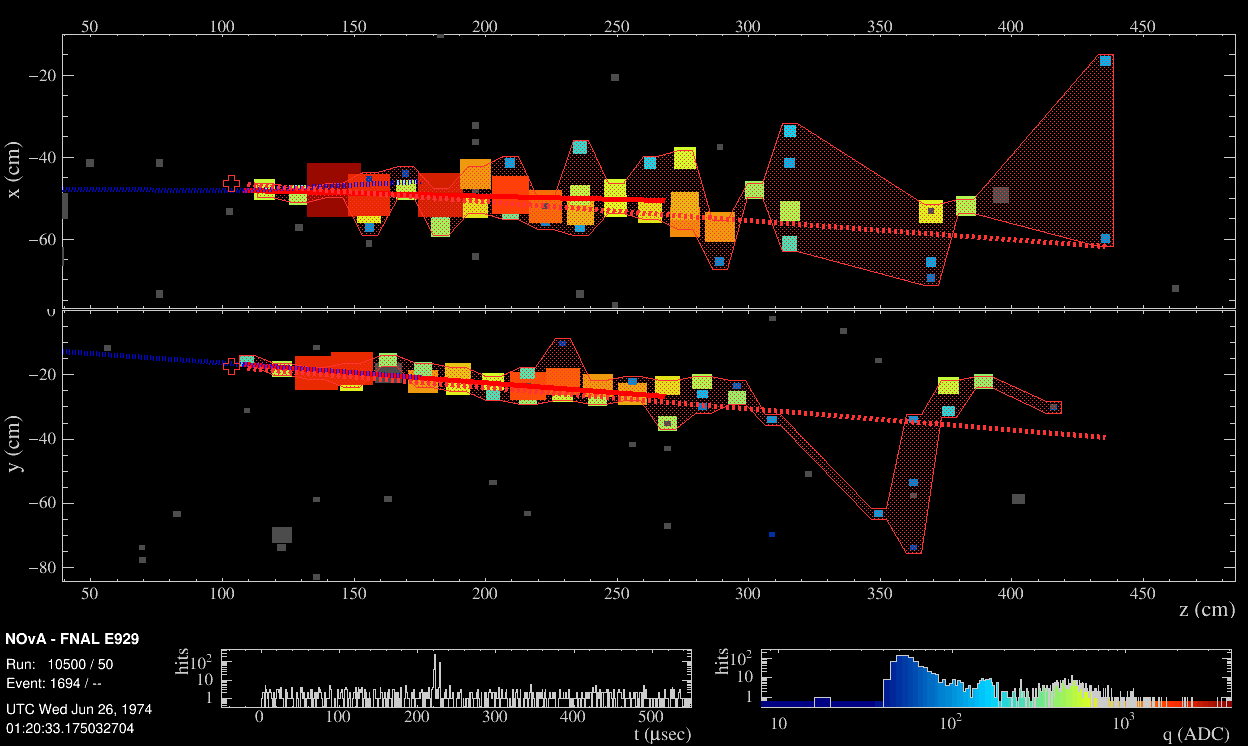
\includegraphics[width=1\textwidth]{Plots/NOvAExperiment/ElectronRecoEVD.png}
\caption[NOvA reconstruction of a single electron]{Reconstruction of a simulated single electron event in the \acrshort{NOvA} \acrshort{ND}. The red cross is the reconstructed vertex, the shaded area shows the cluster of hits into a prong and the dotted red line shows the estimated shower direction. The blue dotted line shows the true direct of the scattering neutrino and the solid red line the true momentum of the scattered electron. Figure from internal \acrshort{NOvA} database \cite{NOvA-doc-13862}.}
\label{fig:NOvARecoEVD}
\end{figure}

For particles that are represented by tracks rather than showers (especially muons), the reconstruction takes the slice hits and forms `Kalman tracks' based on a Kalman filter~\cite{RaddatzNOvAThesis_KalmanTracks.pdf}. In addition to the start point and the direction, which exist also for prongs, tracks also contain information on the vector of trajectory points that make up the track and on the end point - and therefore on the track length. A parallel tracking algorithm takes in the Elastic Arms vertex and the Fuzzy-K prongs and forms \gls{BPF} tracks \cite{BairdNOvAThesis_BPFTracks.pdf,BreakPointFitterBasics.pdf}, using a model of Coulomb scattering and energy loss. \gls{BPF} tracks also contain an information on the particle 4-momenta based on various particle assumptions, most notably the muon assumption. For cosmic particles, mostly muons, \gls{NOvA} uses another track reconstruction algorithm, called `window cosmic track'~\cite{NOvA-doc-15977}. It uses a sliding 5 plane-long window, in which it fits a straight line to the recorded hits. The window starts from the end of the detector and then slides forward and repeats the fitting process until all hits are processed. This way it accounts for possible Coulomb scattering of cosmic muons. The intersection of each cosmic track with the edge of the detector (or extrapolation of the track to the edge of the detector) is reconstructed as the `cosmic ray vertex'.
%%% PID

To identify individual particles and remove backgrounds, \gls{NOvA} uses several \gls{ML} algorithms, outputs of which are used in combination with the information from classical reconstruction algorithms for \gls{PID}. The most common topologies for particles interacting in \gls{NOvA} detectors are shown in Fig.~\ref{fig:NOvAEventTopologies}. Muons are easily identifiable as single long tracks which decay into an electron (or positron) if stopping inside of the detector. Both electrons and $\pi^0$'s produce electromagnetic showers, but thanks to the low-Z composition and high granularity of the detector, there is a gap between the interaction vertex and the electromagnetic shower for the $\pi^0$.

%A Kalman-like algorithm is used with a BDT based on energy loss, multiple scattering, and length parameters of a candidate track to identify muons and reconstruct their energy using track length.

\begin{figure}[ht]
\centering
%is pdf-a
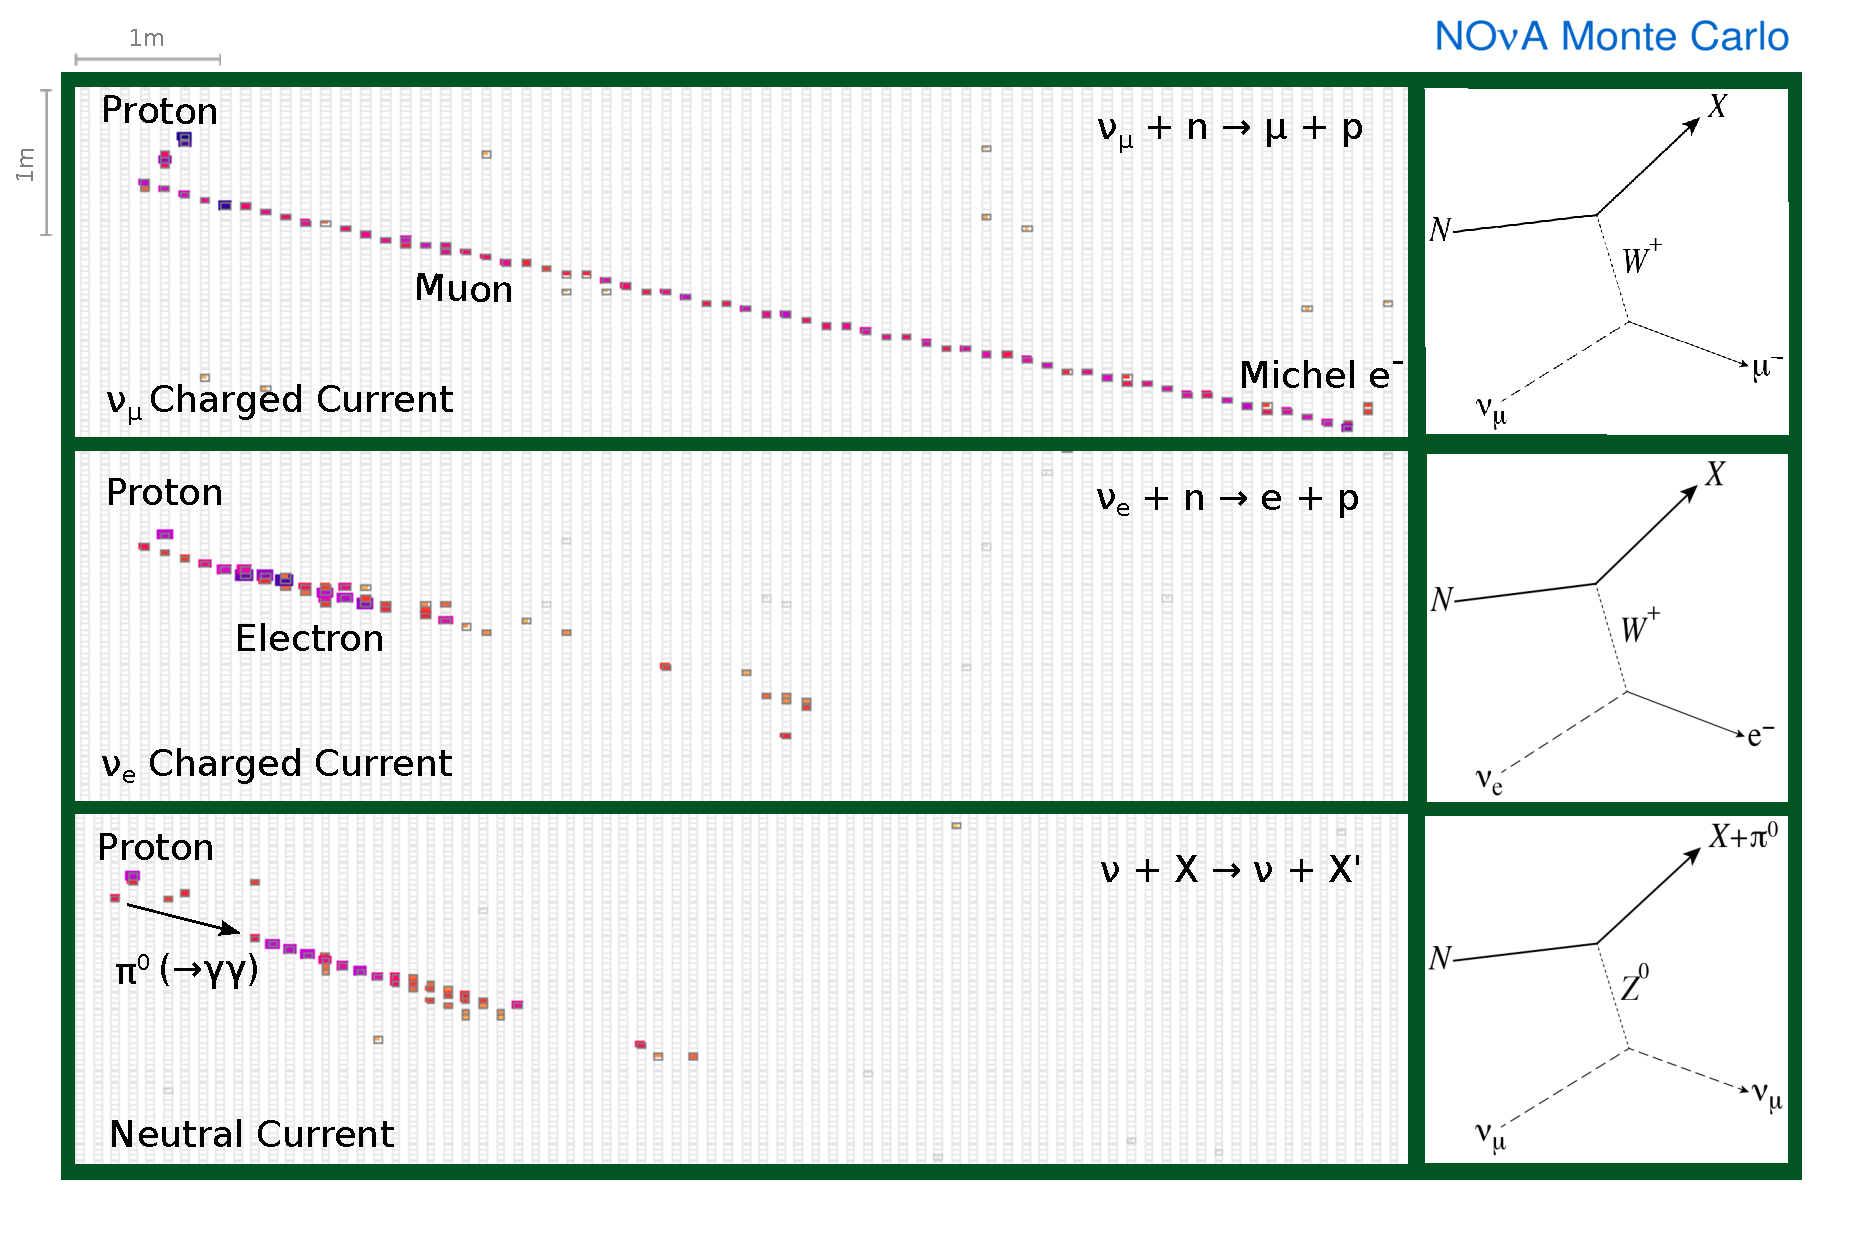
\includegraphics[width=1\textwidth]{Plots/NOvAExperiment/NOvAEventTopology.pdf}
\caption[NOvA detectors event topologies]{Different event topologies as seen in the \acrshort{NOvA} detectors with corresponding Feynman diagrams \cite{NOvAReco.pdf}. Each event is a simulated $\unit[2.15]{GeV}$ neutrino interacting in a \acrshort{NOvA} detector producing a $\unit[0.78]{GeV}$ proton and a second $\unit[1.86]{GeV}$ particle depending on the interactions type. The figure shows only one view and the colouring represents the deposited energy.}
\label{fig:NOvAEventTopologies}
\end{figure}

One of the \gls{ML} algorithms that NOvA employs is a \gls{CNN} based on the GoogLeNet \cite{GoogLeNetArchitecture.pdf} architecture named \gls{CVN} \cite{CVN.pdf}. When it is applied to identify entire events it is called \textit{EventCVN} and uses slice hits to classify interactions into one of the five categories: $\nu_e$, $\nu_\mu$, $\nu_\tau$, \gls{NC}, or cosmic. The same architecture, but applied to the Fuzzy-K prongs, is called \textit{ProngCVN} \cite{PsihasNOvAThesis_ProngCVN.pdf}, and is used to identify what particles the prongs most likely correspond to. This assignment is useful in calculation of prong energy, as described in Sec.~\ref{sec:NOvAEnergyEstimation}. Another \gls{ML} algorithm is specifically designed for identifying muons and is based on a \gls{BDT}. It is called \gls{ReMId}~\cite{RaddatzNOvAThesis_KalmanTracks.pdf} and uses the reconstructed Kalman tracks as inputs.

%From First NOvA results on FHC+RHC: These clusters are categorized as electromagnetic or hadronic in origin using a convolutional neural network (CNN) [Fernanda Psihas thesis]. Hits forming tracks are identified as muons by combining information on the track length, dE=dx, vertex activity, and scattering into a single particle identification (PID) score [Raddatz thesis].

%From NOvAHalfTimeOverview2022.pdf: The energy of charged current neutrino interactions is estimated from the sum of energies of the lepton and the hadronic recoil system. A Kalman-like algorithm is used with a BDT based on energy loss, multiple scattering, and length parameters of a candidate track to identify muons and reconstruct their energy using track length. The energy of electron neutrinos is estimated from a quadratic function of the calorimetric energies of the electron candidate and the hadronic recoil system derived from the simulation [33, 34].

%%%%%%%%%%%%%%%%%%%%%%%%%%%%%%%%%%%%%%%%%%%%%%%%%%%%%%%%%%%%%%%%%%%%%%%%%%%%%%%
%%%%%%%%%                   Detector calibration                     %%%%%%%%%%
%%%%%%%%%%%%%%%%%%%%%%%%%%%%%%%%%%%%%%%%%%%%%%%%%%%%%%%%%%%%%%%%%%%%%%%%%%%%%%%
\section{Detector calibration}\label{sec:NOvACalibration}
%%% General introduction to calibration - why do we do calibration? What do we get from the DAQ?
The energy deposited within \gls{NOvA} detectors is represented by the peak \gls{ADC} values for each cell the particle passed through, obtained from the readout electronics, as described in Sec.~\ref{sec:DAQ}.
The conversion of the peak \gls{ADC} values into physical units of energy requires calibrating the \gls{NOvA} detectors \cite{PrabhjotNOvAThesis_CalibrationAndOscResults2019.pdf}, accounting for the attenuation of light as it propagates through the detector and \gls{WLS} fibres, as well as differences between individual cells and other secondary effects. The purpose of calibration is to calculate a conversion factor from $\unit{ADC}\rightarrow\unit{MeV}$ for every part of the detector, so that the same energy deposited anywhere and at any time, is recorded as the same value of the reconstructed energy.
%By doing this individually for each cell and for small periods at a time, we ensure that energy deposited in any detector, at any place within the detector and at any time, is recorded as the same value in physical units.

%From NOvAHalfTimeOverview2022.pdf: The variations in light output between cells and those due to attenuation along the readout fiber, in both data and simulation, are calibrated using cosmic-ray muons. The overall energy response of the detectors is calibrated using stopping muon tracks along a window from 200 cm to 100 cm before the end of the track. The absolute energy scale is cross-checked and bench marked against simulation using beam-induced protons, muons, and neutral pions at the Near Detector.

%make sure that we get the same amount of energy wherever or whenever it's deposited in whichever of NOvA's detectors and to express this amount of energy in physical units. The NOvA calibration uses cosmic ray muons, which provide a consistent, abundant, and well-understood source of energy deposition.

%%% Calibration samples, trigger, reconstruction, and selection. Also simulation, fiber brightness and so on...
\gls{NOvA} uses cosmic ray muons for calibration due to their abundance in the \gls{NOvA} detectors and their consistent energy deposition. To calculate the absolute energy scale, \gls{NOvA} selects a subsample of muons stopping inside of the detectors when they are almost exactly \gls{MIP} and therefore have a well understood energy deposition. The cosmic muons are collected using a periodic trigger (see Sec.~\ref{sec:DAQ}) with the same length as the beam trigger, whilst removing events with timestamps overlapping with the beam spill window. The simulation of cosmic muons is created using the \gls{CRY}~\cite{CRY} \gls{MC} generator, as outlined in Sec.~\ref{sec:NOvASimulation}.

%[NOvAResultsNuOnly2018.pdf] Separate periodic minimum-bias triggers of the same length as the beam trigger allow us to collect high-statistics cosmic data for algorithm training and calibration purposes.

Cosmic muon tracks are reconstructed using the window cosmic track algorithm described in Sec.~\ref{sec:NOvAReconstruction}. The window cosmic track algorithm is highly efficient and pure, with $97\%$ of tracks reaching at least $90\%$ efficiency (fraction of true particle hits assigned to the track) and over $99\%$ maintaining at least $90\%$ purity (fraction of track hits from the correct particle)~\cite{NOvA-doc-15977}. Spatially, $93\%$ (X view) and $95\%$ (Y view) of hits lie within $\unit[6]{cm}$ of the track. The algorithm also achieves good endpoint resolution, with a mean z-resolution of $\unit[4.24]{cm}$, making it effective for identifying stopping tracks essential for calibration.

The selection of well reconstructed cosmic tracks requires that at least $80\%$ of all hits from the reconstructed slice contribute to the track \cite{NOvA-doc-13579-FACalorimetricEnergyScale}. Each track must have at least 2 hits in both the x and y views and the difference in the number of planes the track crossed between the views must be at most $10\%$ of the total number of planes. Also, the plane where each track starts or stops in one view must be within 3 planes of the start or stop plane in the other view. Additionally, since tracks that do not cross many planes tend to not be reconstructed very well, the extent of each track in the z direction must be at least $\unit[70]{cm}$ and tracks must have at least $20\%$ of their total track direction in the z axis. Tracks with on average more than 6 cells per plane and with path lengths through the cell larger than $\unit[10]{cm}$ are removed for the same reason. Furthermore, all the reconstructed tracks must start at most $\unit[10]{cm}$ from the edge inside of the detector and stop at most $\unit[10]{cm}$ outside of the detector. Lastly, tracks with trajectory points far away from each other are also removed, resulting in a total $\sim 90\%$ efficiency of the track selection. The selection of stopping muons for the absolute energy scale relies on identifying Michel electrons, which are produced by decaying muons at the end of their tracks, as can be seen on the top panel of Fig.~\ref{fig:NOvAEventTopologies}.

Since the energy deposited in a cell is proportional to the distance the particle travels through the cell, the input variable for calibration is the deposited energy divided by the path length through the cell $\unit{\gls{PE}/cm}$. To ensure the path length is well calculated, all hits used in calibration must satisfy the so-called `tricell' condition, shown in Fig.~\ref{fig:NOvATricellCondition}. This means that for each calibration hit, there must be a corresponding hit in both of the surrounding cells in the same plane for the same track. The path length can then be calculated simply from the height of the cell and the angle of the reconstructed track. In case there is a bad channel in a neighbouring cell (right side of Fig.~\ref{fig:NOvATricellCondition}), this channel is ignored and the tricell condition looks one cell further \cite{PrabhjotNOvAThesis_CalibrationAndOscResults2019.pdf}. If the tricell condition fails, the hit can still pass the `z tricell' condition, which is a longitudinal equivalent of the tricell condition and requires a hit in both the neighbouring planes in the same view and with the same cell number. The `z tricell' hits are saved separately and may be used if there are no hits satisfying the original tricell condition. This is especially useful for the cells on the edge of the detector, which fail the tricell condition due to only having one neighbouring cell.

\begin{figure}[hbtp]
\centering
\begin{subfigure}[b]{0.49\textwidth}
\centering
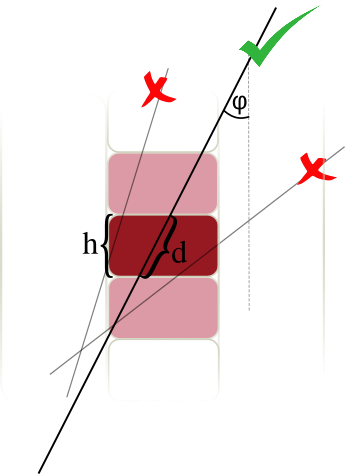
\includegraphics[width=0.6\textwidth]{Plots/NOvAExperiment/TricellConditionWithDescription.png}
\end{subfigure}
\begin{subfigure}[b]{0.49\textwidth}
\centering
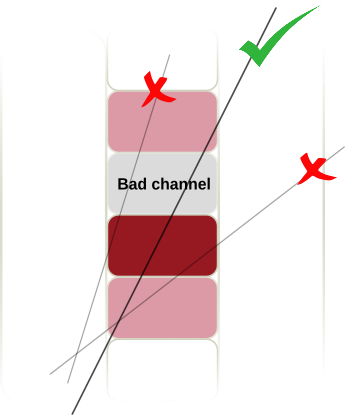
\includegraphics[width=0.6\textwidth]{Plots/NOvAExperiment/TricellConditionWithBadChannel.png}
\end{subfigure}
\caption[Tricell condition for calibration hits in NOvA]{Illustration of the tricell condition. Only the hits with two surrounding hits in the same plane are used in the \acrshort{NOvA} calibration, as shown on the left plot. This is to ensure a good quality of the path length (d) reconstruction, which is calculated from the known cell height (h) and the reconstructed track angle $\left(\varphi\right)$. In case the hit is next to a bad channel, as shown on the right plot, the bad channel is ignored and the tricell condition requires a hit in the next cell over.}
\label{fig:NOvATricellCondition}
\end{figure}

%The first step in the attenuation calibration is to select the suitable hits from tracks of cosmic ray muons. Because a reliable estimate of pathlength is required, not all hits are suitable for use.  If a cell has each of its neighbors in the same plane hit, then we know, for a Y view cell, that the track entered through the upper wall, and exited through the lower wall. The pathlength then is just the width of the cell divided by the direction cosine. This selection also significantly decreases the chance that the hit in question is a noise hit. Allowance is made for neighboring dead cells, so e.g. “hit, dead, hit, hit” would still lead the 3rd cell to be selected. The second best hit selection, in cases where there are too many dead neighboring cells on each side, is the so-called “z” estimator, where a hit is required at the same cell number in each of the neighboring planes in the same view. The pathlength is then the ratio of cell depth to cz.[docdb:13579 - SA The Attenuation and Threshold Calibration of the NOvA detector, copied from docdb:7410]

%from docdb:7410: A requirement that the track be “throughgoing” (lowest endpoint outside the fiducial volume) was applied, but doesn’t make much difference. I think this selection was broken by the recent changes to StopperSelection anyway. (So it seems that it was required for the relative calibration that the muons are through-going, but I assume this was discarded somewhere down the line)

%Stopping muon selection (from docdb:13579 - FA\_Calorimetric\_energy\_scale): There are two avenues for selecting stopping muons; i) selecting tracks whose reconstructed end point is contained within the detector and ii) selecting tracks that have a Michel electron at one end. Michel electrons are useful for both identifying muons and effective tagging of the end point of muon tracks. The stopping selection requires the reconstructed end point of the muon track to be at least 50 cm from the detector edge. The identification of a Michel electron at the end of a muon track has two stages of both temporal and spatial range requirements. Firstly, a candidate Michel electron hit is required to occur between 1 and 30 microseconds after the mean time of the hits on the track. Furthermore, the candidate Michel electron must be within a 30 cm sphere surrounding the reconstructed track end point. The candidate Michel electron hit for a muon track is the hit that produces the largest detector response among the hits that pass the above cuts. Secondly, cell hits surrounding the candidate Michel electron hit are associated with the Michel electron if they occur within a 30 cm sphere surrounding the Michel electron candidate. Furthermore, to be associated with the Michel electron the cell hits must occur between 0.5 microseconds before and 0.5 microseconds after the candidate Michel electron. Michel electrons at the end of muon tracks are reconstructed using the candidate and associated Michel electron hits. The stopping muon selection requires a Michel electron at the end of the muon track.

%Calibration is necessary to convert electronic signals to physically meaningful energy in units of GeV. Two calibration steps precede the calorimetric energy calibration. First raw ADCs (Analogue Digital Conversion) are converted to units of photo-electrons (PE) using the known average response of the APDs; secondly an attenuation calibration corrects for the position dependent response [6]. A drift calibration may be included in the future to correct for changes in detector response over time. The calorimetric energy scale calibration is the last step in the calibration chain and the detector response should already be uniform in space and eventually also in time. [docdb:13579 - FA\_Calorimetric\_energy\_scale]

%Using the average expected APD response, integrated charge from the ADCs are converted to units of photo-electrons (PE) [SA Absolute energy scale]

The calibration conversion factor from the signal recorded by the detector readout to the deposited energy can be expressed by as
\begin{equation}\label{eq:NOvACalibration}
E_{dep}\ \left[\unit{MeV}\right]=\textsf{Signal}\ \left[\unit{ADC}\right]\times S_d\times TS_{d,i}^{\textsc{Calib}}\times R_{d,i}\left(t\right)\times A_d\left(t\right).
\end{equation}
The calibration scale therefore consists of four separate and complementary factors: the Scale $\left(S_d\right)$, the Threshold and Shielding correction $\left(TS_{d,i}\right)$, the Relative calibration $\left(R_{d,i}\left(t\right)\right)$ and the Absolute calibration $\left(A_d\left(t\right)\right)$, all described below. Each part is calculated for each detector separately, as indicated by the subscript $d$. The threshold and shielding correction is only used during calibration and is omitted when applying the calibration results. The relative and absolute calibrations are calculated for each time period separately to account for possible changes in the energy deposition throughout the time, possibly caused by the ageing of the scintillator oil, or of the readout electronics. The time periods are either determined by a fixed time interval (one month for \gls{FD} and \gls{ND}), or by running conditions separated by significant changes to the readout or the \gls{DAQ} systems, including the summer shutdown.

The threshold and shielding correction and the relative calibration calculate a calibration factor for each position within the detector to account for variations caused by the attenuation of light as it travels through the \gls{WLS} fibres, or by differences between individual cells. This is expressed with a subscript $i$ in Eq.~\ref{eq:NOvACalibration}. For data, the position of a hit in the detector is described by the plane number, cell number and the position within the cell $\left(w\right)$. $w$ is calculated as the projection of the cosmic track to the central cell axis and its value is equivalent to the x axis (y axis) coordinate of the projection for the horizontal (vertical) cells, with the 0 value at the centre of the cell \cite{PrabhjotNOvAThesis_CalibrationAndOscResults2019.pdf}.

%The light is attenuated while traveling through the fiber. To find the correct energy of the incident particle these losses are corrected by using cosmic ray muons. The cosmic ray muons are used to calibrate the NOvA detectors because they provide a source of consistent energy across the detectors. The purpose of the attenuation calibration is to provide constants and formulae such that an amount of energy deposited in the detector and registered by an APD can be expressed in comparable units, PECorr which are the corrected photo-electrons (PE) no matter where the deposition occurred. Variations in time are to be handled by the drift calibration. The purpose of the absolute calibration is to provide a scaling factor, independent of channel since all of that variation should have been taken out by the relative calibration, so that energy deposits can be expressed in physically meaningful units (GeV).
%For both purposes cosmic rays are used as probes. For the attenuation calibration they represent a source of consistent energy deposits across the detector of approximately 1 minimum ionizing particle’s energy, MIP, but this is not assumed. Any average value consistent across the detector would do. For absolute calibration, stopping muons are used, whose precise energy deposits should be estimateable from the Bethe Bloch formula. [docdb:13579 - SA The Attenuation and Threshold Calibration of the NOvA detector, but a lot of this is actually just copied from Backhouse's original calibration technote docdb:7410]

%(Dividing data into periods and epochs) A new period is started for a major change to running conditions such as a horn current change, a long shutdown, target replacement, etc. Periods are divided into epochs. A new epoch is started whenever analysis or production reasons dictate. Calibration has been performed for all the periods separately and has used the data that are determined by the Data Quality group to be good. The effects of aging, temperature, partial filling, and cooling are neglected. The drift calibration should be able to account for all of these (but drift calibration doesn't really exist yet afaik). [docdb:13579 - SA The Attenuation and Threshold Calibration of the NOvA detector]

For simulation, the calibration does not use the plane number to determine the position within a detector, as by construction all detector planes should have the same readout. This significantly reduces the requirements for the number of events that need to be simulated, reconstructed, and calibrated, especially for the \gls{FD} with 896 planes. However, in reality there are some variations in the detector response between individual planes, caused by different \textit{brightness} qualities of the fibres, zipped or twisted fibres, different qualities of the scintillator, possible air bubbles, and potentially other factors. To include these differences in simulation without having to simulate every cell individually, all the cells are divided into 12 equally populated \gls{FB} bins based on
the uncorrected average response in the center of that cell, as shown in Fig.~\ref{fig:NOvAFiberBrightness}. These \gls{FB} bins describe the relative differences in the detector response between individual cells \cite{NOvA-doc-34909}.

%\cite{NOVA-doc-13579-SAAttenuationAndThreshold,NOVA-doc-34909}.

\begin{figure}[hbtp]
\centering
\begin{subfigure}[b]{0.495\textwidth}
\centering
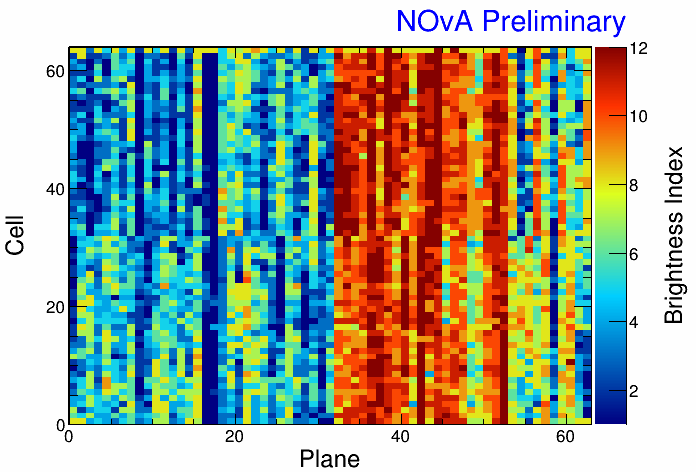
\includegraphics[width=\textwidth]{Plots/NOvAExperiment/BrightnessIndex.png}
\end{subfigure}
%\hfill
\begin{subfigure}[b]{0.495\textwidth}
\centering
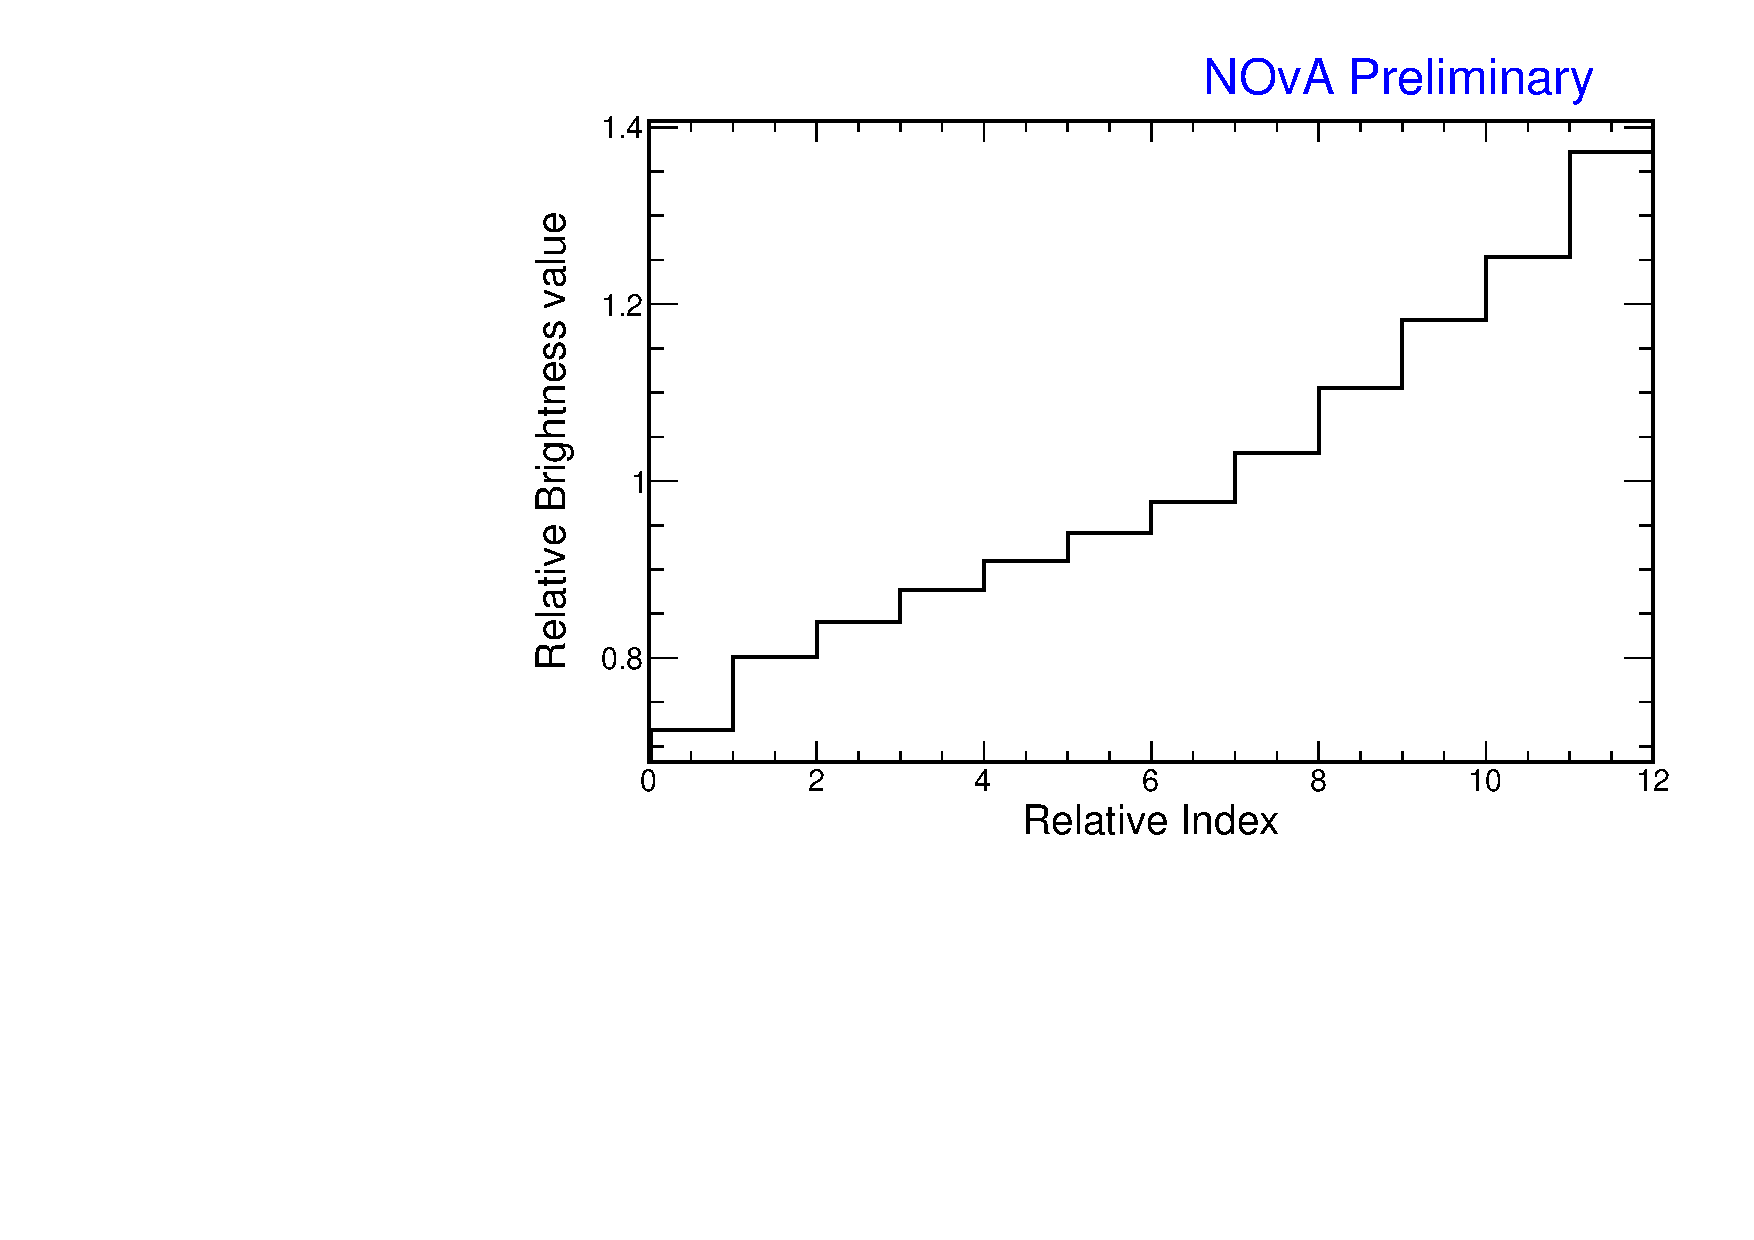
\includegraphics[width=\textwidth]{Plots/NOvAExperiment/BrightnessIndexToValue.pdf}
\end{subfigure}
\caption[Fibre Brightness bins for the NOvA calibration]{Distribution of the \acrshort{NOvA} detector cells into 12 brightness bins (left plot), each representing a relative difference in energy response (right plot) due to different brightnesses of the fibres, scintillators, or readout. This is an example from the \acrshort{NOvA} Test Beam detector, described in Sec.~\ref{sec:TBExperiment}, where the left side of the detector (planes 1-32) has clearly lower response relative to the right side of the detector (planes 33-64).}
\label{fig:NOvAFiberBrightness}
\end{figure}

%To divide each detector into the 12 brightness bins, we use results from the relative calibration. Specifically we take the result of the attenuation fit (equal to the average response) in the centre of each cell to fill a 2D histogram. Then we normalize this histogram by dividing the response in each $\textsf{Cell}\times\textsf{View}\times\textsf{Plane}$ by the average response in the corresponding $\textsf{Cell}\times\textsf{View}$. All uncalibrated cells get assigned the average response (1 in normalized histogram). Then we make a 1D histogram filled with the normalized responses of each cell and divide this histogram into 12 equally populated bins (so each bin represents approximately the same number of detector cells, shown on the left plot of Fig. \ref{figFiberBrightnessBins}). The mean normalized response in each bin represents the relative brightness value of this bin (right plot of Fig. \ref{figFiberBrightnessBins}).

\subsection{Scale}
The scale calibration factor from Eq.~\ref{eq:NOvACalibration} is a simple conversion from the peak \gls{ADC} value into the number of \glspl{PE}. This factor only depends on the \gls{APD} gain (which was different in the beginning of \gls{NOvA} data taking) and on the \gls{FEB} type (different between detectors, as described in Sec.~\ref{sec:DAQ}).

%I think I should actually include some kind of a description of the ADC to PE conversion.
\iffalse
The scaling of the ADC to PE depends only on the gain and the version of the FEB. Otherwise it's just a very simple scaling (explain this at the PE definition):
\begin{equation}
PE=\frac{\textsf{peakADC}}{\textsf{ADCPerPE}},
\end{equation}
\begin{equation}
\textsf{ADCPerPE}=\textsf{Gain}\times\frac{4095}{ADCScale}
\end{equation}
where ADCScale is 217000 for FEBv4.1 and 204800 for FEBv5.2.
\fi

%The PECorr scaling is 75.0 (NDOS), 37.51 (ND), 39.91 (FD) and 39.91 (TB)

\subsection{Threshold and shielding correction}\label{sec:NOvACalibTSCorr}
%[CalibrationFirstTechnote2014.pdf] There are three main assumptions for calibration: response is stable in time (drift), the energy spectrum of cosmic rays is uniform in space (shielding), the ADC response to arriving photons is linear
The threshold and shielding correction accounts for two assumptions, which hold true in most cases in \gls{NOvA}, but fall short for some hits at the bottom of the detector, or far away from the readout, especially for the \gls{FD} \cite{PrabhjotNOvAThesis_CalibrationAndOscResults2019.pdf}.

The first assumption is that the \gls{ADC} response to the photon signal is linear, which is mostly true except close to the \gls{APD} threshold. Energy deposited far away from the readout may produce photons that get attenuated enough to be shifted below the threshold. However, due to natural fluctuations of the number of photons created by the energy deposition, the same deposited energy may also produce photons that would make it over the threshold, therefore making it appear that the actual deposited energy was higher then in reality, introducing a bias to the calibration. The threshold correction is calculated using simulation, as the ratio between the mean of the Poisson distribution of the true number of the created \gls{PE} $\left(\textsc{PE}_{\mathrm{Poisson}\lambda}\right)$ and the number of the `reconstructed' \gls{PE} seen by the \gls{APD} $\left(\textsc{PE}_{\mathrm{Reco}}\right)$.

The second assumption is that the spectrum of cosmic muons is uniform within each detector. Again, this is generally true, but breaks down in the \gls{FD}, which is big enough for the top of the detector to shield the bottom of the detector and therefore affect the energy distribution. The shielding correction is calculated from simulation as a ratio between the expected deposited energy if the particle was a \gls{MIP} $\left(E_{\textsc{MIP}}\right)$, which is estimated from simulation for the \gls{NOvA} scintillator as $E_{\textsc{MIP}}=\unit[1.78]{MeV/cm}$ and the true deposited energy $\left(E_{true}\right)$.

The total threshold and shielding correction is calculated for simulated events in each cell, \gls{FB} bin and $w$ as
\begin{equation}\label{eq:NOvAThresholdShieldingCorrection}
TS_i = \frac{\textsc{PE}_{\mathrm{Poisson}\lambda}}{\textsc{PE}_{\mathrm{Reco}}}\frac{E_{\textsc{MIP}}}{E_{True}}.
\end{equation}
To ensure that the correction changes smoothly across each cell position, the final correction is calculated as a fit to the mean correction value along $w$ in each cell and \gls{FB} bin.

%Similar effect, specifically for the vertical cells, is caused by using cosmic muons for calibration and applying it to beam muons. The top of the detector effectively shields the bottom, skewing the energy distribution of cosmic muons. To correct for both of these effect, we use the simulation pclist sample to calculate the threshold and shielding (also called threshold and shadowing) correction by comparing the true and reconstructed information. We apply this correction before the attenuation fits \cite{NOVA-doc-13579-SAAttenuationAndThreshold}.

%Should I write anything more? Maybe about how do we calculate this more specifically, or that it's done for view X fb bin X cell X w

%In the Far Detector data and MC a large divergence between calibrated and true energies as a function of W was observed [8]. This was traced back to the much longer cell lengths in the FD meaning that thresholds play a large role at the foot of a cell. Also self-shielding of the detector by its own mass lay a role in the observed discrepancy. Thresholds mean that for a hit to be seen by an APD, it may need to have a slight upwards fluctuation in the number of photons produced by the energy deposition. Self-shielding means that the average visible energy depositions from MIPs are not truly spatially uniform in the detector. If not corrected for these effects, there will be a bias in the set of hits that the attenuation fit sees, and leads it to overestimate the light-level, and so under-estimate real hit energies by tens of percent. The approach adopted to solve this problem was to create a correction factor as a function of view, cell, and position along the cell which would be applied before the attenuation correction to remove the effect of thresholds and shielding. To this end MC truth information about the calibration hit sample is used to create a combined threshold and shadowing correction for each cell and view combination,
%\begin{equation}
%T=\frac{PE}{\lambda}\frac{E_{true}}{E_{mip}},
%\end{equation}
%where $T$ is the combined “threshold and shielding” correction factor, $PE$ is the simulated photoelectrons recorded at the readout, $\lambda$ is the number of simulated photons which would be seen at the readout out in the absence of fluctuations, $E_{true}$ is the true energy deposited in the cell and $E_{mip}$ is the naive energy you would expect to be deposited based on the pathlength through the cell. In this way it encodes a threshold correction based on the simulated readout PE with and without the fluctuations, with $\lambda$ dependent on your simulated threshold, as well as a shielding correction based on the simulated energy deposition and a naive no shielding approximation. This equation gives us a cell by cell correction but we use an empirical polynomial fit to that distribution which removes statistical noise from the correction and well describes the initial distribution. This correction factor is applied to the cell by cell data and MC PE/cm distributions before the attenuation fits. [docdb:13579 - SA The Attenuation and Threshold Calibration of the NOvA detector, reference 8 is for docdb:7247, a talk by Backhouse]

\subsection{Relative calibration}\label{secRelativCalibration}

%The \textbf{relative calibration} corrects for attenuation of scintillator light as it travels through the cell to the readout, as well as for differences between detector cells. This correction is calculated for each cell separately.

%Detailed description can be found in the "Instructions for the Attenuation Calibration Job" technote from Prabhjot from docdb:13579 (list of all calibration technotes) and on the relative calibration wiki page.

The main goal of the relative calibration is to correct for the attenuation of the scintillator light as it travels through the \gls{WLS} fibre to the readout. The attenuation in each cell is estimated by performing an `attenuation fit' to the mean response in $\unit{\gls{PE}/cm}$, as shown in Fig.~\ref{fig:NOvACalibrationAttenuationFit}. The relative calibration scale is then calculated as the ratio between the average response in $\unit{\gls{PE}/cm}$ across the entire detector (can differ between detectors) and the result of the attenuation fit in each particular position within the detector. The response after applying the relative calibration scale is expressed as \glspl{PECorr}. Since the relative calibration scale is calculated for each cell independently, it effectively corrects for the relative differences between detector cells as well as for the attenuation. Therefore, the resulting distribution of $\unit{\gls{PECorr}/cm}$ should be uniform across the detector, especially along the plane, cell and $w$ \cite{PrabhjotNOvAThesis_CalibrationAndOscResults2019.pdf}.

%by fitting the average detector response over the position in each cell, separately for every cell inside each detector. Dividing the "average response" of the detector by the result of the attenuation fit for each $\textsf{Plane}\times\textsf{Cell}\times\textsf{w}$ combination effectively removes relative differences within and between all cells across the entire detector. The average response is a single constant number chosen to approximately represent the average response in the middle of the cell. Its value is for the far detector and Test Beam 39.91~PE/cm and for the near detector 37.51~PE/cm. The value of the average response has no impact of the calibration results, as the absolute scale of the detector response is determined during the absolute calibration and relative calibration only serves to remove the relative differences \cite{NOVA-doc-7410,NOVA-doc-13579-SAAttenuationAndThreshold}.

The first step to do the attenuation fit is to create `attenuation profiles' for each cell. Attenuation profiles are profile histograms of mean detector response over the path length through the cell, in the units of $\unit{\gls{PE}/cm}$, along the position within the cell. An example attenuation profile is shown in Fig.~\ref{fig:NOvACalibrationAttenuationFit} as black dots. The threshold and shielding correction described in Sec.~\ref{sec:NOvACalibTSCorr} is applied to the attenuation profiles before doing the attenuation fit, which consists of two steps.

\begin{figure}
    \centering
    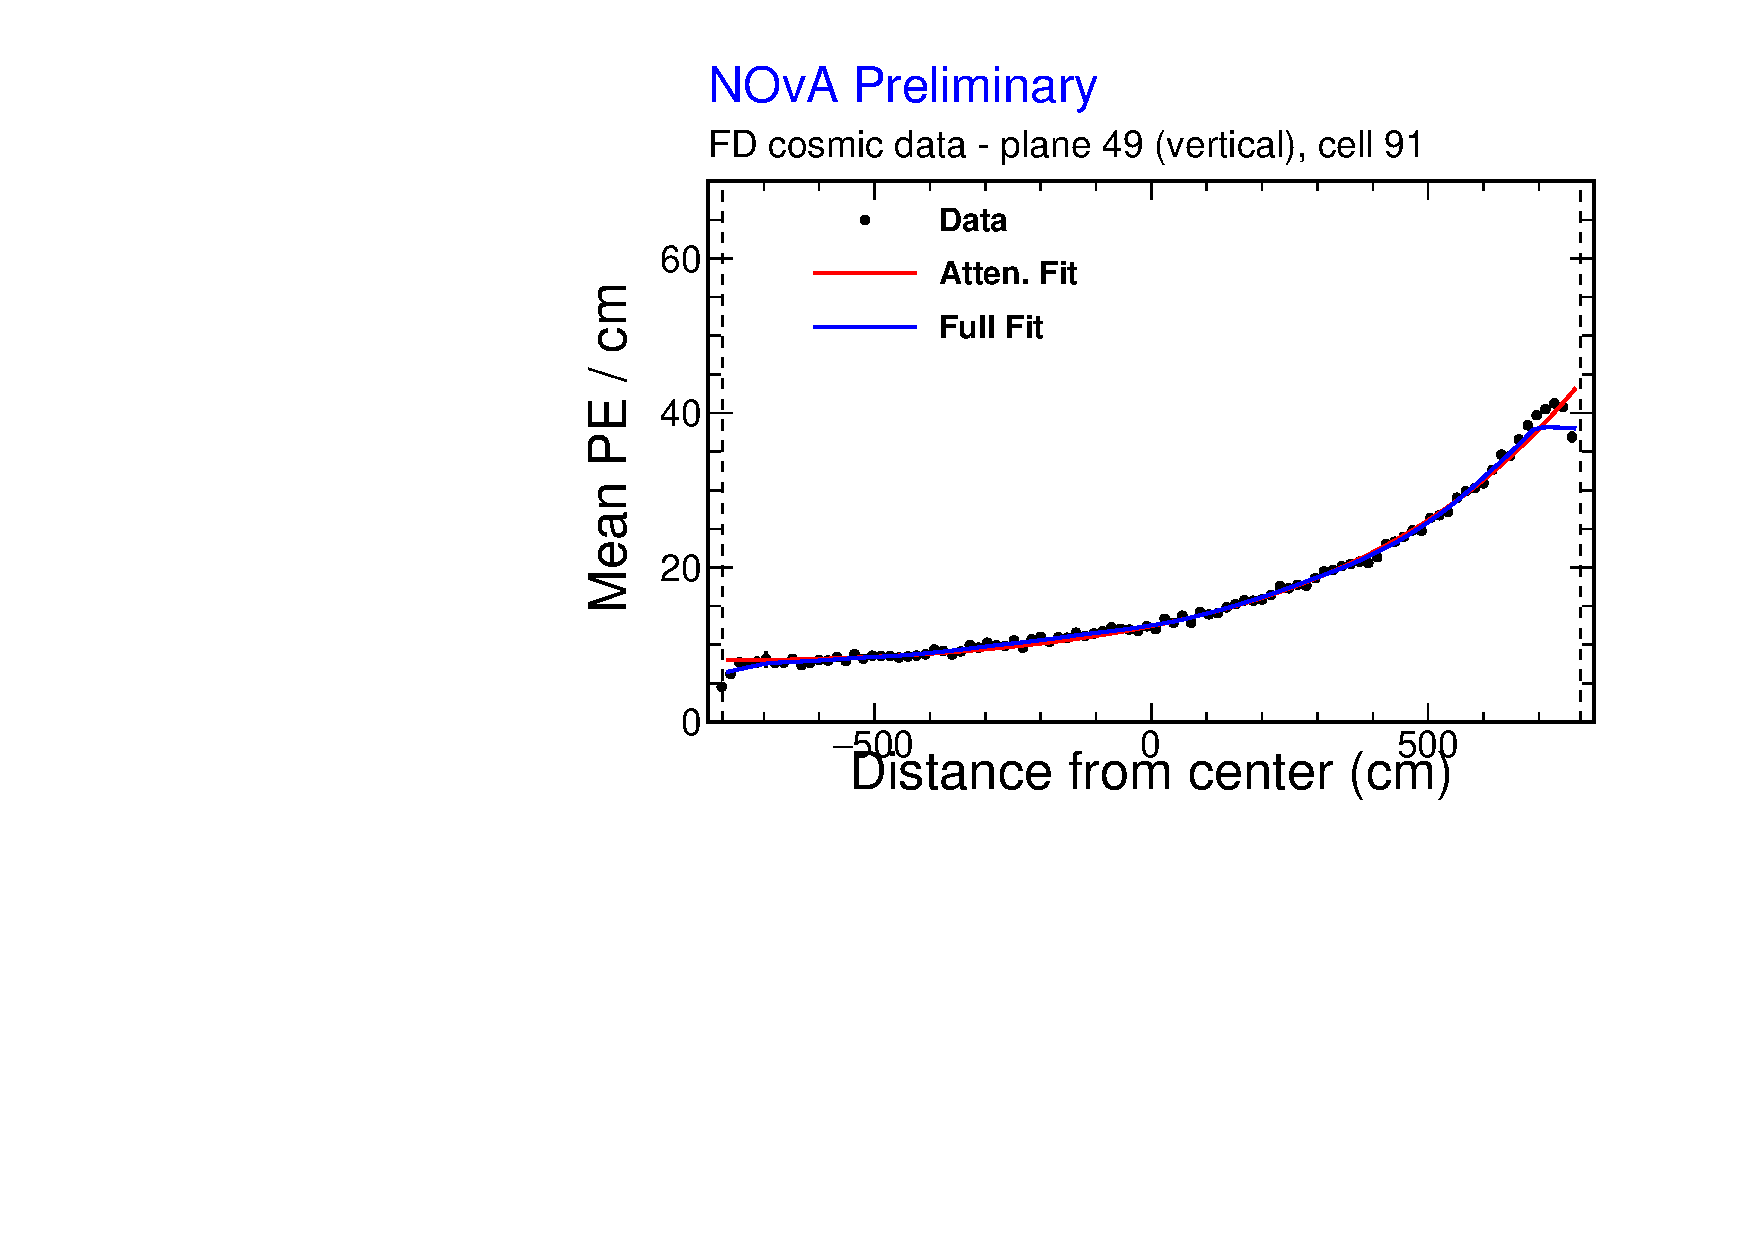
\includegraphics[width=.7\textwidth]{Plots/NOvAExperiment/ExampleAttenuationFit.pdf}
    \caption[Example attenuation fit for NOvA relative calibration]{Example attenuation fit for a single cell in the \acrshort{NOvA} \acrshort{FD} across its full length, as shown by dashed vertical lines. The red line shows the initial exponential fit and the blue line shows the full fit after the \acrshort{LOWESS} correction, both described in text. The noticeable drop in $\unit{\gls{PE}/cm}$ at the edges of the cell is caused by a combination of low statistics (due to the hit selection as outlined in text) and physical effects of \gls{WLS} fibre loop ends and connections to the readout. Figure from \cite{totfit_fd_datafitX_049_091.pdf}.}
    \label{fig:NOvACalibrationAttenuationFit}
\end{figure}

\begin{enumerate}
\item The first step is a three-parameter exponential fit that models light attenuation along the \gls{WLS} fibres. Since light can travel either directly to the readout or loop around the far end of the cell, the fit includes two corresponding exponential components:
\begin{equation}\label{eq:NOvARelCalibExpFit}
y=C+A\left(\exp\left(\frac{w}{X}\right)+\exp\left(-\frac{L+w}{X}\right)\right),
\end{equation}
where $y$ is the fitted response, $L$ is the length of the cell and $C$, $A$ and $X$ are the fitted parameters representing the background, attenuation scale and attenuation length respectively. An example of the exponential fit is shown as a red curve in Fig.~\ref{fig:NOvACalibrationAttenuationFit}.
\item The second step is the smoothing out of residual differences between the exponential fit and the original distribution with the \gls{LOWESS} method, shown in Fig.~\ref{fig:NOvACalibrationLOWESSCorrection}. The residual differences get evened out by creating a smooth distribution of 20 locally weighted points across the length of each cell. The result of the \gls{LOWESS} correction is then combined with the exponential fit into the full attenuation fit, shown as a blue line in Fig.~\ref{fig:NOvACalibrationAttenuationFit}.
\end{enumerate}

\begin{figure}
    \centering
    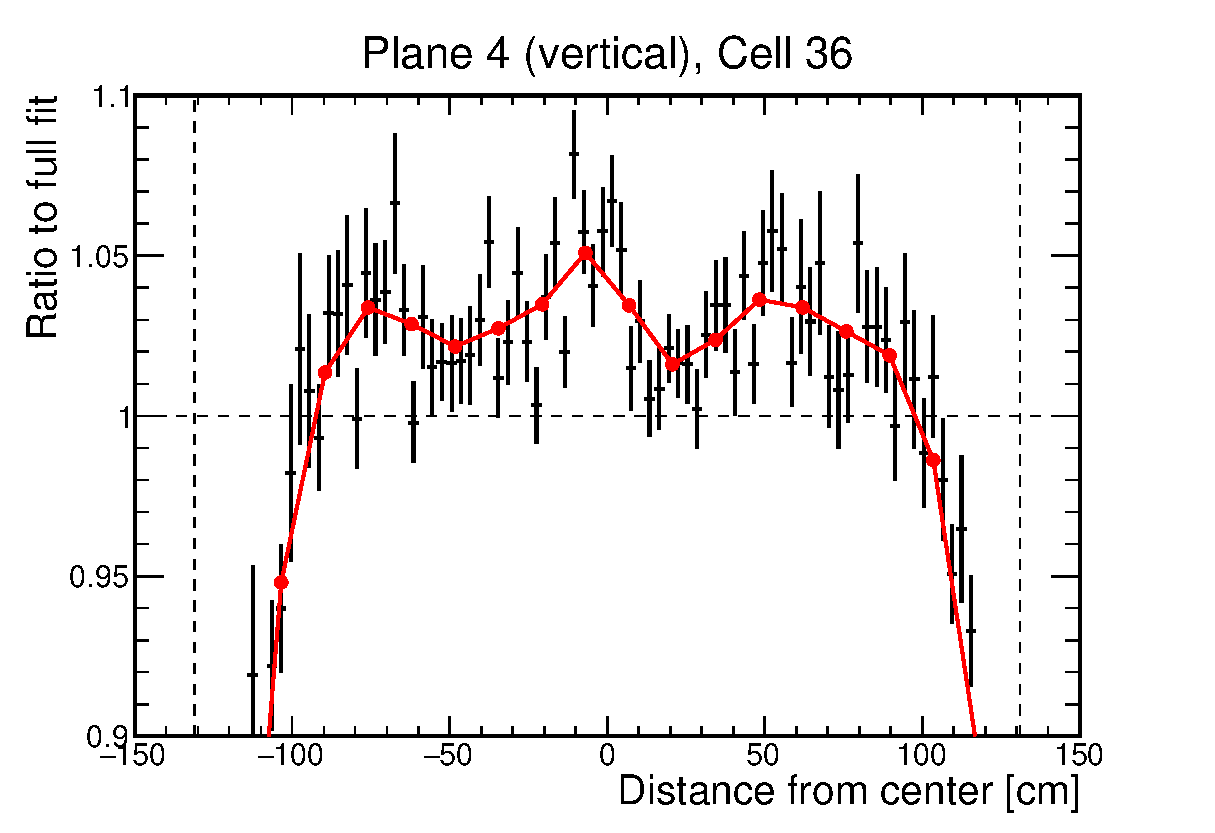
\includegraphics[width=.7\textwidth]{Plots/NOvAExperiment/ExampleLOWESSFit.eps}
    \caption[Example LOWESS correction for NOvA relative calibration]{Example \acrshort{LOWESS} correction for the residual differences after the exponential part of the attenuation fit of the \acrshort{NOvA} relative calibration. This is an example for a single cell in the \acrshort{NOvA} Test Beam detector with black points showing the residual differences and red line the \acrshort{LOWESS} correction, both described in text.}
    \label{fig:NOvACalibrationLOWESSCorrection}
\end{figure}

Even after applying the \gls{LOWESS} correction, there are sometimes large differences between the attenuation fit and the fitted response. This is usually caused by a small number of events in that cell, common for cells at the edge of the detector. To ensure a good quality of the attenuation fit, a $\chi^2$-equivalent (divided by the number of degrees of freedom) metric\footnote{The metric used to assess calibration correctness is calculated as the sum of the squared differences between the bin content and the fit result, normalized by the bin content, averaged over all bins. Since this is functionally equivalent to a reduced $\chi^2$ (i.e., $\chi^2$ divided by the number of degrees of freedom) metric, we refer to it as $\chi^2$ throughout this thesis.} between the attenuation fit and the fitted response is calculated and only cells with the final $\chi^2\leq 0.2$ are counted as \textit{calibrated}. Cells with $\chi^2>0.2$ are ignored in further processing and marked as \textit{uncalibrated}. About $99\%$ cells in the \gls{FD} pass this calibration condition \cite{NOvA-doc-13579-Second}.

%Attenutation profiles have a constant binnin fNBins=100 (in w), same for ND, FD and TB. This results in an effectively finer binning for TB compared to ND and FD. For FD w = (-900,+900), ND: (-250,+250), TB: (-150,+150). TB: 3cm/bin, ND: 5cm/bin, FD: 18cm/bin. What effect could this have on the relative calibration results? Particularly on the calibration shape?

%where y is the response, L is the cell length, C, A and X are the free parameters in the fit. X gives the attenuation length as well. Initially, the fit is to the central part of the cell, which is different for each detector. In addition to the approximately quartic behavior at the ends of every channel there are in many channels fairly large residuals. They don’t appear to follow any consistent pattern. The leading hypothesis is that these are due to varying fiber position within the cell. Usually the fiber lies in the corners of the cell, but if it is somehow twisted so that it rises into the center of the cell, then it should collect more light, to an extent comparable to what is seen here. To remove such an irregular pattern, the residual from the analytic fit is simply fit with LOcally WEighted Scatter plot Smoothing, LOWESS. The LOWESS curve at each point is formed from the weighted mean of the deviations. The weighting function is the traditional tri-cube, (insert equation, likely not needed for this technote) [docdb:13579 - SA The Attenuation and Threshold Calibration of the NOvA detector, already in 1stAna and Backhouse's technote]

%For NDOS the fit was a very little bit different, where we didn't use $L$ but $3L/2$. Also it says that "Over the length of an NDOS cell, the effect of the long attenuation length is imperceptible, and is modelled as a constant (If you put a long attenuation term in, the fit drives the length scale to infinity anyway). [docdb:7410]

%In many channels, fairly large residuals are visible. They don’t appear to follow any consistent pattern. The hypothesis is that these are due to varying fibre position within the cell. Usually the fibre lies in the corners of the cell, but if it is somehow twisted so that it rises into the centre of the cell, then it should collect more light, to an extent comparable to what is seen here. To remove such an irregular pattern, the residual from the analytic fit is simply fit with LOWESS (locally weighted scatterplot smoothing). The LOWESS curve at each point is formed from the weighted mean of the deviations. The weighting function is the traditional tri-cube:
%\begin{equation}
%w_i=\left(1-\left|\frac{x-x_i}{\sigma}\right|^3\right)^3.
%\end{equation}
%The smoothing length scale $\sigma$ is 30cm. 20 points calculated by this method are stored, to be linearly interpolated between to approximate the full LOWESS curve. If the LOWESS fit at any point exceeds 15\% the original attenuation fit was very bad, and the channel is marked uncalibrated. Figure 4 shows an example of large (10\%) deviations being fitted. This variation is not seen in the MC, and so the LOWESS fit is skipped there. Due to the lower stats available in MC, instead of being collated by plane and cell, the curves are only calculated by view and cell. [docdb:7410]

%The current value of $\sigma$ in the code is $1.5\times\textsf{DetWidth}/20$

\subsection{Absolute calibration}
%Followed by the \textbf{absolute calibration}, which only uses stopping muons when they are minimum ionising particles. In the absolute calibration we calculate a scale between the measured energy deposition, corrected by the relative calibration, and the simulated energy deposition in physical units of $\unit{MeV}$. This scale is calculated for each time period and each detector separately, which ensures the energy deposition is directly comparable wherever or whenever it occurred.

The absolute calibration only uses hits from muons stopping inside of the detector, in a track window $\unit[1-2]{m}$ from the end of their tracks. This is when they are approximately \gls{MIP} and their energy deposition is well understood. Additionally, hits at the edges of each cell are removed to mitigate the  effects at the end of the \gls{WLS} fibres and the lower number of events at the edge of the detector \cite{NOvA-doc-13579-FACalorimetricEnergyScale}. Thanks to this selection, it is not necessary to apply the threshold and shielding correction for the stopping muon hits.

First, the relative calibration results are applied to the selected stopping muon hits to get a distribution of the corrected detector response in $\unit{\gls{PECorr}/cm}$, as shown on the left of Fig.~\ref{fig:NOvACalibrationAbsoluteEnergyScale}. The mean of this distribution is called the \textit{reconstructed} \gls{MEU} and is calculated separately in each of the two views, and in each time period or version of simulation. Analogously, the mean of the true deposited energy in $\unit{MeV/cm}$ from simulation, shown on the right of Fig.~\ref{fig:NOvACalibrationAbsoluteEnergyScale}, is called the \textit{true} \gls{MEU}. The absolute energy scale (the absolute calibration scale) is then the ratio between the true and the reconstructed \gls{MEU} value, where both  the \gls{MEU} values are taken as a simple average over the two views
\begin{equation}\label{eq:NOvAAbsEnergyScale}
\textsf{Absolute Energy Scale} = \frac{\textsc{MEU}_{\mathrm{True}}\ \left[\unit{MeV/cm}\right]}{\textsc{MEU}_{\mathrm{Reco}}\ \left[\unit{\textsc{PECorr}/cm}\right]}.
\end{equation}

\begin{figure}
    \centering
    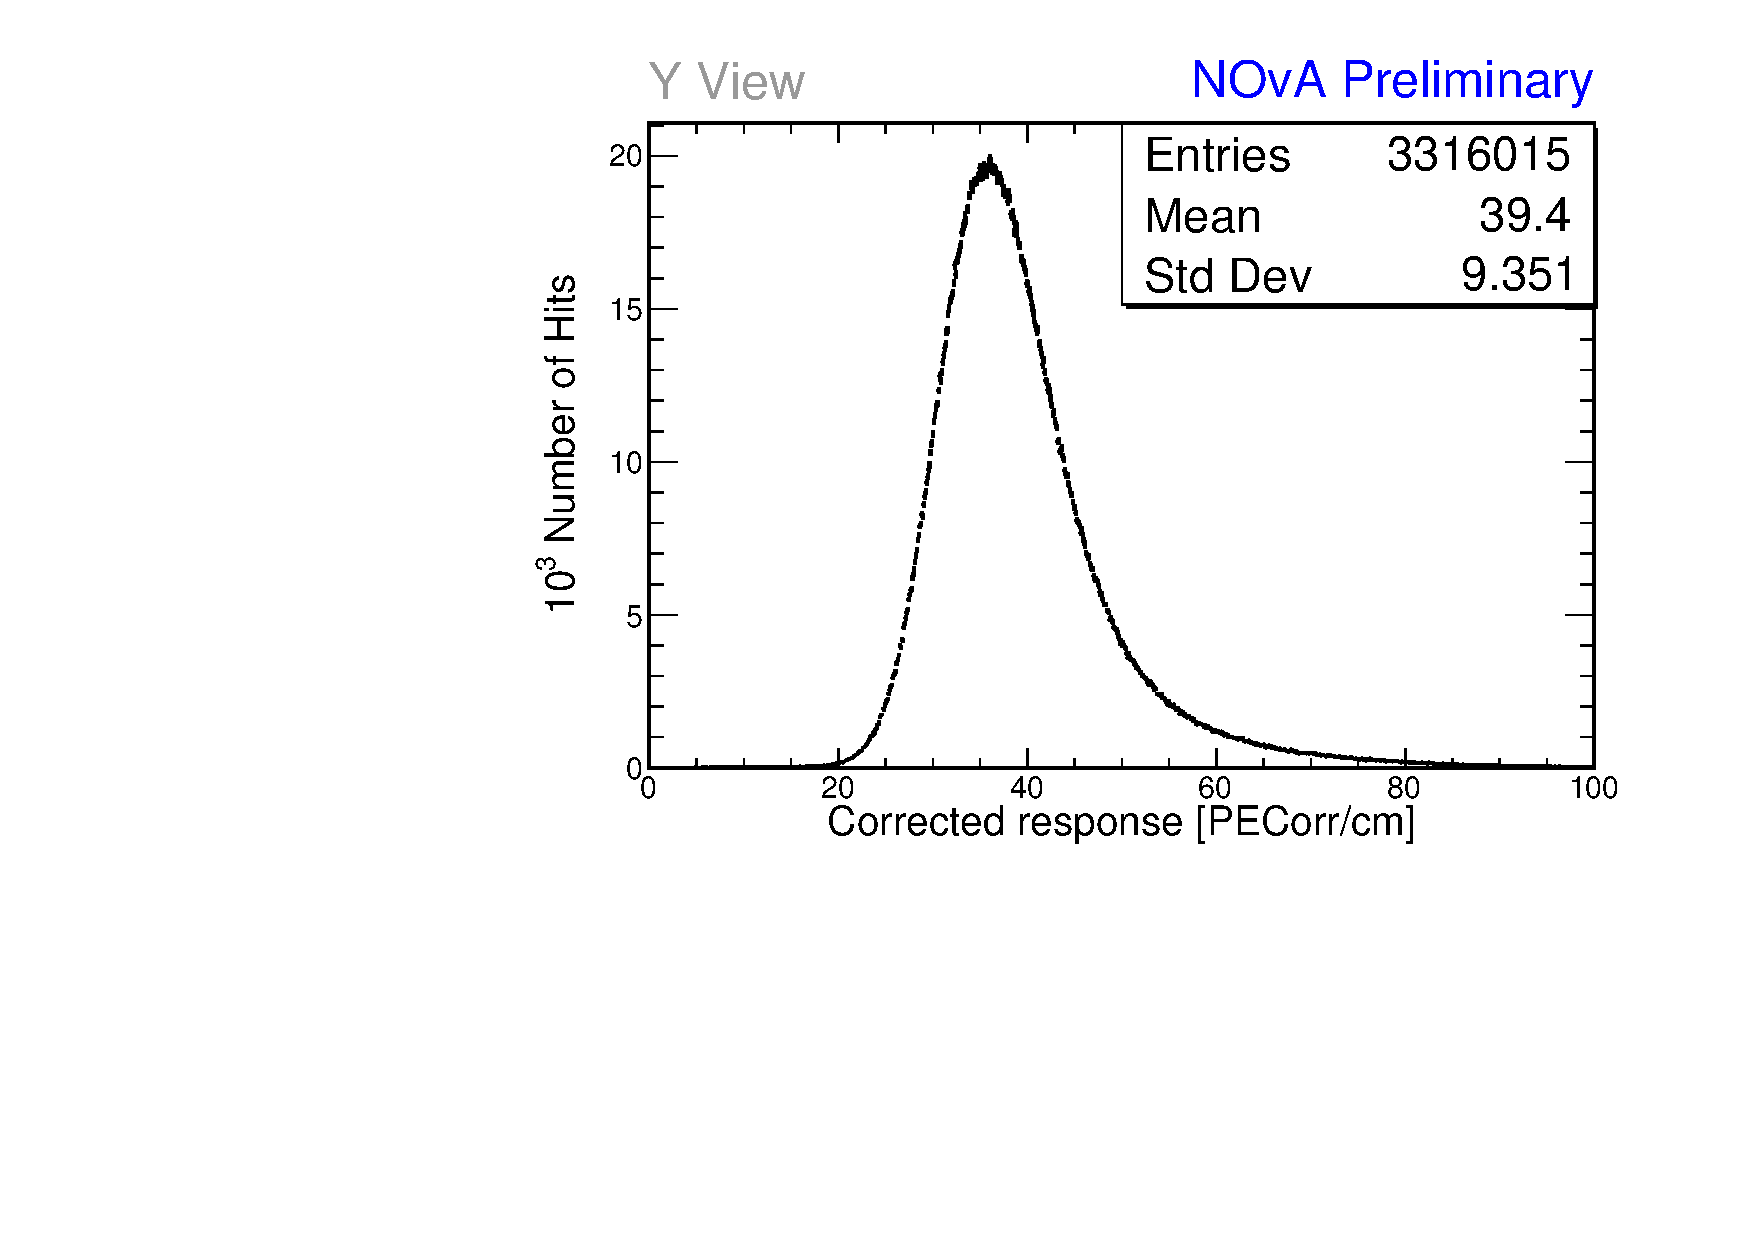
\includegraphics[width=0.49\textwidth]{Plots/NOvAExperiment/ExampleAbsCalib_P4_meu_y.pdf}
    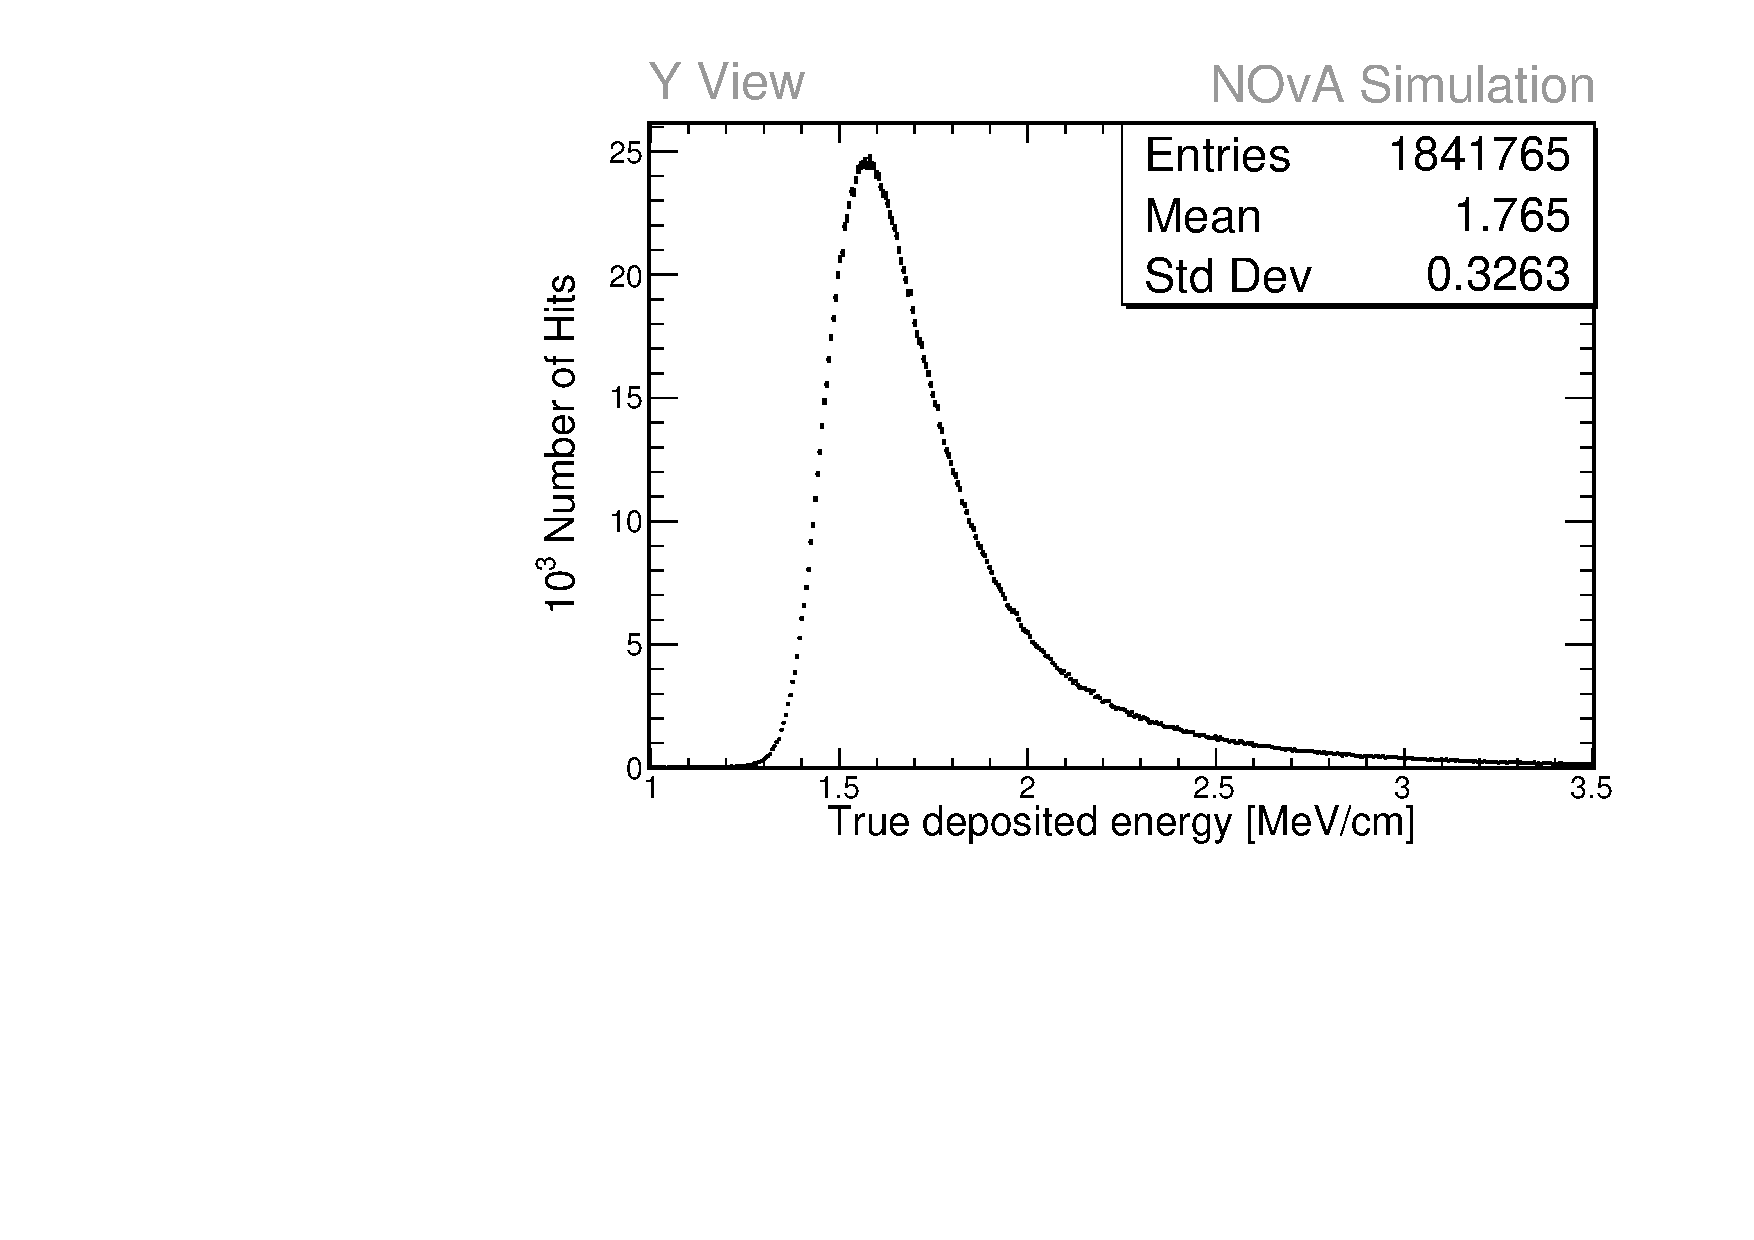
\includegraphics[width=0.49\textwidth]{Plots/NOvAExperiment/ExampleAbsCalib_Sim_mev_y.pdf}
    \caption[Example distributions for the NOvA absolute calibration]{The absolute energy scale is calculated as the ratio between the simulated mean true deposited energy (right) and the mean reconstructed energy response (left) for selected stopping muons in each view and each data period or simulation.}
    \label{fig:NOvACalibrationAbsoluteEnergyScale}
\end{figure}

%For each calibrated data and simulation sample we take a mean of the corrected deposited energy distribution, separate for each view. We then take a simple average from the two views to get the final $\textsf{MEU}_{reco}$ in units of $\unit{PECorr/cm}$ for each sample \cite{NOvA-doc-13579-FACalorimetricEnergyScale}. Additionally, from simulation we can get the mean of the distribution of the true deposited energy in the scintillator, $\textsf{MEU}_{truth}$ in units of $\unit{MeV/cm}$ for the same sample of stopping muons. 

The values of the absolute energy scales for each data period and simulation, as well as the results of the attenuation fit, are saved in a set of lookup tables, which are then used any time a hit is recorded in the \gls{NOvA} detector and processed and reconstructed with the \gls{NOvA} algorithms described above.

The performance of the \gls{NOvA} calibration procedure is assessed by comparing calibrated energies between data and simulation for several `standard candle' interactions. These differences define the absolute scale systematic uncertainty (Sec.~\ref{sec:NOvASystematics}). The calibration also corrects for spatial variations in energy deposition, with residual variations quantified under the calibration shape systematic uncertainty. By calibrating in small time intervals, we account for temporal energy variations, with remaining effects included in the detector ageing systematic uncertainty.

%Stopping muons provide a good sample of known energy deposits. If we can collect a “golden” sample, they should provide the scale factor to convert PECorr to GeV. So far, the method used has been imperfect, and the absolute calibration constants are known to be off by approx. 10\%. Since a factor already has to be derived to correct for dead material, this is not significantly impeding current efforts, but work was recently gone into improving this area. [docdb:7410 - this was likely before the track window cut was introduced] (Here it says that it's not such a big a problem since we have to scale for the dead material anyway. But nowadays we have to account for a large systematic uncertainty in the absolute energy scale in our analyses. How is the dead material correction different from the energy scale uncertainty?)

%...the calibration of the calorimetric energy scale of the NOvA detectors uses the energy deposited by stopping muons as a standard candle. To reduce systematic uncertainties, only those energy deposits in a 1-2 m window away from the muon track end point are used. The mean of the detector response distribution is found for data and MC in both near and far detectors. The mean of the distribution of true energy deposits in the track window is used to provide a conversion factor between the detector response and the true energy deposited in the scintillator for minimum ionising muons. The simulated dE/dx is uniform within about 1.8\% for hits around the minimum between 100-200 cm from the track end. The energy that a muon deposits within each cell is estimated using Geant 4 and stored in Fibre Liquid Scintillator (FLS) hits. FLS hits are only those within the active material (liquid scintillator) and energy loss within the passive material (plastic extrusions) is ignored. an estimate of the minimum energy loss rate of stopping muons in the NOvA scintillator is found to be,
%\begin{equation}
%\left.\frac{dE}{dx}\right|_{\textsf{mip}}=\left(1.7915\pm 0.0035\right)\unit{MeV/cm}.
%\end{equation}
%For stopping muons in NOvA it is also important to consider their decay. The muon has a vacuum lifetime of about 2.2 microseconds and favourably decays, with a branching ratio approx. 100\%, into an electron, an electron anti-neutrino and a muon neutrino. The electron produced in this decay is called a Michel electron and is used to select muons that stop within the NOvA detectors. The energy scale calibration is performed using cosmic ray muons. The calibration measures the detector response in data and MC in both near and far detectors and normalises them all by providing a conversion factor, for all four cases, that converts the detector response to energy in GeV. The energy loss rate (dE/dx) of stopping muons is well described by the Bethe-Bloch and is a function of the distance from the stopping point. A track window technique is used to minimise the variations in detector response that depend on the distance to the track end. Using this technique only hits within a region of distances from the track end are used. The position of the track window is chosen such that a mis-reconstruction of the track end point has the minimum effect on the mean detector response. The track window is currently set to be in the range from 100 cm to 200 cm from the track end.[docdb:13579 - FA\_Calorimetric\_energy\_scale]

\section{Energy estimation}\label{sec:NOvAEnergyEstimation}
The deposited energy from detector calibration (Sec.~\ref{sec:NOvACalibration}) is only the first step in estimating the neutrino energy $\left(E_\nu\right)$ required for the main \gls{NOvA} analyses.

For the $\nu_\mu$ disappearance analysis, the $\nu_\mu$ energy is measured as the sum of the muon energy and the energy of the hadronic shower \cite{NOvAResults2021.pdf}. The muon energy is identified from the length of its track, without the need of the calibration results. The energy of the hadronic shower is estimated from simulation as a fit to the 2D distribution of the true $\nu_\mu$ energy minus the reconstructed muon energy, versus the visible (not corrected for the dead material) deposited energy of the hadronic system \cite{PsihasNOvAThesis_ProngCVN.pdf}.

For the $\nu_e$ appearance analysis, the $\nu_e$ energy is calculated using a quartic fit to the 2D distribution of the electromagnetic versus the hadronic calorimetric energies, both corrected for the energy deposition in the dead material (\gls{PVC} cells) \cite{PsihasNOvAThesis_ProngCVN.pdf}. The dead material correction is currently just a simple scaling of the deposited energy from calibration for all particles and is calculated from the measurement of the $\pi^0$ mass peak in the \gls{NOvA} \gls{ND}. This correction is correct only for electromagnetic showers and is not directly applicable to hadronic showers. The fit to determine the $\nu_e$ energy keeps the normalization of both the electromagnetic and the hadronic energies free, so the exact value of the dead material correction is not important. It is however used in other, non-neutrino oscillation analyses.

\section{Systematic uncertainties}\label{sec:NOvASystematics}
%%% Introduction - what categories are there and which ones are significant
There are several known unknowns that can affect the results of \gls{NOvA} measurements, represented by systematic shifts of predictions. The impact of systematic uncertainties is assessed by varying prediction independently for each systematic shift and passing all predictions through the same analysis procedures as the nominal (non-shifted) sample. The nominal and systematically shifted predictions are then compared to determine the systematic uncertainty on the measured parameters. This approach inherently accounts for the effects of systematic uncertainties on background composition, event selection, reconstruction, and other aspects of the analysis.

The primary sources of systematic uncertainties in \gls{NOvA} include the simulations of neutrino flux, neutrino interaction, and detector modelling, all explained in Sec.~\ref{sec:NOvASimulation}, as well as the detector calibration procedure. Other sources of systematic uncertainties are relevant only to specific analyses and are not discussed here. In \gls{NOvA}, the 3-flavour \cite{NOvAResults2021.pdf} and the sterile \cite{NOvASterilesFHCRHCResults2021.pdf} neutrino oscillation analyses use the \gls{ND} data to constrain the \gls{FD} prediction by fitting the \gls{ND} prediction to data, significantly reducing the effect of the neutrino beam and neutrino interaction systematic uncertainties. On the other hand, these are the leading sources of systematic uncertainties for the \gls{ND}-only analyses, such as the cross section analyses \cite{NOvANCPi0XSecMeasurement2019.pdf, NOvANumuCCXSexMeasurement2023.pdf, NOvANueCCXSecMeasurement2023.pdf, NOvANuMuCCPi0XSecMeasurement2023.pdf}, or the neutrino magnetic moment analysis. Detector calibration and modelling uncertainties are significant across all \gls{NOvA} measurements.

%Systematic uncertainties in \gls{NOvA} analyses arise from the imperfect knowledge on the individual components of the \gls{NOvA} experiment, or from the known shortcomings of the prediction used to extract the measured parameters. Even though different analyses in \gls{NOvA} need to consider different systematic uncertainties and their effect on the results varies, there are a few commonalities across all \gls{NOvA} analyses that are explained below.

%%% Treatment of systematics in NOvA - predictions and fits - nuisance parameters


%\gls{NOvA} in general applies the systematic uncertainty by shifting the nominal prediction and passing the shifted prediction through all the \gls{NOvA} mechanisms the same way as the nominal prediction. Then, we compare these shifted and propagated predictions with the nominal one and their difference is our systematic uncertainty. These systematic uncertainties are included in the parameter estimation and in the fits in general via nuisance parameters. The main systematic uncertainties can be grouped into the neutrino beam uncertainty, neutrino interaction uncertainty, detector modelling uncertainty, and calibration uncertainty. There are other analysis specific or sub-dominant systematic uncertainties which are not described here, such as the neutron uncertainty, the near-far detector differences, lepton reconstruction (muon energy scale and angle), normalization.

%\cite{NOvAResults2021.pdf} The impacts of systematic uncertainties are evaluated by varying the simulation via event reweighting or simulating alternative event samples and repeating the extrapolation procedure.
%\cite{NOvANueCCXSecMeasurement2023.pdf}  Systematic uncertainties are evaluated by varying the parameters used to model neutrino flux, neutrino-nucleus interactions (nu-A), detector response, and re-extracting the differential cross section. The difference between the cross section extracted using the nominal simulation and that extracted using the simulation with a varied parameter is taken as the uncertainty due to each parameter. The procedure accounts for changes in the compositions of backgrounds, selection efficiency, and event reconstruction due to the variations considered.
%\cite{NOvAResultsNuOnly2018.pdf} We evaluate the effect of potential systematic uncertainties on our results by reweighting or generating new simulated event samples for each source of uncertainty and repeating the entire measurement, including the extraction of signal and background yields, the computation of migration matrices, and the calculation of the ratios of FD to ND expectations using each modified simulation sample and applying our constraint procedures.


%%% NEUTRINO FLUX UNCERTAINTY
The systematic uncertainty on the neutrino beam prediction arises from two sources: hadron production and beam focusing \cite{NuMIFlux.pdf}. Hadron production uncertainties are estimated using the multi-universe technique within the \gls{PPFX} (see Sec.~\ref{sec:NOvASimulation}), which involves creating 100 alternative universes where inputs from external measurements of hadron production cross-sections are varied within their respective uncertainties. Beam focusing uncertainties are contained in 20 parameters accounting for uncertainties in horn and target positions, horn current, beam position on the target, beam spot size, and the effect of Earth's magnetic field in the beam pipe. Since all these uncertainties can be correlated, particularly in an off-axis detector such as \gls{NOvA}, a \gls{PCA} is performed to estimate the bin-to-bin covariances in true energy for each neutrino flavour, detector and beam mode \cite{NitishOscMeasuremetPCAStatisticalAna2021.pdf}. \gls{PCA} reduces the number of required neutrino flux systematic uncertainty parameters from $20\times100$ to only $8$ \textit{`principal components'} (each with positive and negative shifts) for the \gls{ND} analyses, or $5$ principal components for the \gls{ND}+\gls{FD} analyses. Additionally, principal components are uncorrelated by construction and ordered by the scale of their effect on the neutrino beam prediction.

%[Maria thesis]  The effects of these uncertainties are correlated between true neutrino energy bins. To reorganize these into uncorrelated systematic uncertainties, these are treated with a technique called Principal Component Analysis (PCA) [102]. This method starts from a statistical ensemble of randomly generated variations in these uncertainties in order to estimate the variance in each neutrino energy bin as well as the correlations between different bins. A covariance matrix is then obtained and diagonalized, and the 5 eigenvectors with the largest eigenvalues are considered for this analysis, as they capture 97.5\% of the variance.

%[NosekThesisNOvAOscillationSysts2021.pdf]
% General notes on the PCA can be found in, e.g., Ref. [229], a simpler tutorial in Ref. [230], for PCA in the NOvA neutrino oscillation analyses see Refs. [231, 232, 233, 234], or see Appendix B.

%From docdb:54582: NOvA analyses use two sets of flux uncertainties: beam transport, which cover differences between the simulation and the working conditions of the NuMI beam, and hadron production, which concern the rates of production of pions and kaons from proton collisions on the carbon target. The beam transport uncertainties include the horn and target position, the horn current, the beam position on the target, the beam spot size, and the effect of the Earth’s magnetic field in the beam pipe (which is not simulated in G4NuMI). The effect of each uncertainty is below 5% at the flux peak for both the ND and FD. PPFX is used to constraint the hadron production models for the NuMI beam using external hadron production data and theory. The systematic effect is assessed by generating 100 universes where the uncertainty on the external data and theoretical assumptions are allowed to float. Flux uncertainties are known to show correlations across most neutrino energy bins, especially in off-axis measurements like NOvA. NOvA looks at 100 PPFX universes, and for each PPFX universe we further sample the beam transport parameters 20 times, creating a total of 2000 universes representing many different possibilities of the flux uncertainty. These universes are used to estimate the bin-to-bin covariances in true energy for each neutrino flavour, detector and beam mode. A Principal Component Analysis (PCA) is applied to the covariance matrices to find sets of uncorrelated shifts - Principal Components (PCs). The covariance matrices for each neutrino flavour and beam mode are calculated in the (ND, FD/ND) basis to represent the approximate extrapolated error at the Far Detector. These are then diagonalized to give the Principal Components, given by the eigenvectors i.e, $PC_i=\sqrt{\lambda_i}v_i$, where $\lambda_i$ represents the $i$-th largest eigenvalue and $v_i$ its corresponding eigenvector. The components are then converted to the (ND, FD) basis. Each PC can be used as a systematic shift in the oscillation fit with a pull of $1\sigma$. By ordering each of the PCs in terms of the magnitude of their eigenvalues, one can also capture most of the information embedded in the covariance matrix with just a few components. Five principal components are used in the oscillation fit. The hadron production uncertainty on the neutrino flux is evaluated using a "multi-universe" technique. This is $\sim 7\%$ at the spectrum peak dominated by interactions where relevant data to be included in the constraining procedure is currently not available (mostly mesons and proton quasi-elastic interactions). Beam transport uncertainties are incorporated by propagating uncertainties in the alignment of beamline elements, including the beam position on the target, the horns current and position, the beam spot size, and the effect of the Earth magnetic field in the decay pipe. The beam optic uncertainty is $\sim 4\%$ at the peak.

%Not sure if I should include a discussion on nu-on-e, or low nu studies here, or just PPFX improvements.

%%% Neutrino interaction systematic uncertainties
Neutrino interaction-related systematic uncertainties involve 77 adjustable parameters, most of which are provided directly by GENIE \cite{GENIE.pdf} to account for the theoretical uncertainties of the prediction \cite{NOvAResults2021.pdf}. These include knobs to adjust the axial and vector masses of \gls{QE} and \gls{Res} interactions, $\pi$ angular distribution in the \gls{Res}$\pi$ production, parameters of the Bodek-Yang \gls{DIS} model, or branching ratios for the radiative and single $\eta$ resonance decays. Additionally, \gls{NOvA} developed its own set of systematic uncertainties \cite{NOvANuIntUncertaintiesFromNDData2020.pdf}, either based on its own measurements, or on discrepancies observed in other experiments. For example, the \gls{NOvA} \gls{MEC} tune has associated uncertainties based on its dependence on the transferred four momentum or on the neutrino energy. Furthermore, a discrepancy between data on the \gls{Res} interactions at low transfer energies and their prediction in the \gls{NOvA} \gls{ND} motivated a conservative $\unit[100]{\%}$ one-sided systematic uncertainty, allowing for a complete suppression of \gls{Res} events with low energy transfers.

%[NOvAResults2021.pdf] Neutrino interaction model uncertainties are evaluated using the event reweighting framework in GENIE with additional uncertainties constructed by NOvA as follows.
%[NOvAResultsNuOnly2018.pdf] Estimates for the majority of the cross section and FSI uncertainties that we consider are obtained using the event reweighting framework in GENIE [15].
% GENIE based systematics
%Many of these parameters are provided by GENIE in the form of parameter scales for the physical inputs, such as: \cite{GENIE.pdf} tweaking the axial and vector masses for CC and NC resonant interactions, form factors for the elastic NC interactions, parameters of the Bodek-Yang DIS model, branching ratios for the radiative and single $\eta$ resonance decays, pion angular distribution in the resonant single pion production, or CCQE axial form factor normalization.

% NOvA MEC tune

%\cite{NOvANuIntUncertaintiesFromNDData2020.pdf} However, we substitute our own treatment in several instances where different uncertainties are warranted, as described in the following sections. Significant disagreement with the ND data remains even after combining any of the MEC models available in GENIE with the prediction after the modifications described above, as can be seen in Fig. 3. We introduce Three 2p2h uncertainties: one covering uncertainty in target nucleons, one addressing uncertainties in the energy dependence of the cross section, and one treating uncertainties in the (q0, q) response (all uncorrelated).

%Additionally, there are uncertainties developed by the \gls{NOvA} cross section group to account for our changes to the original GENIE configuration and to the discrepancies we saw in our measurements or elsewhere. The custom \gls{NOvA} \gls{MEC} tune has an associated uncertainties based on its dependence on the transferred four momentum, or neutrino energy.

%[NOvAResults2021.pdf] Neutrino interaction model uncertainties are evaluated using the event reweighting framework in GENIE with additional uncertainties constructed by NOvA as follows. Uncertainties on CCQE RPA, low-Q2 RES suppression, 2p2h, and nonresonant and incoherent N$\pi$ production are established for the new model set using methods similar to those in Ref. [84].

%[NOvAResultsNuOnly2018.pdf] as the detailed nature of MEC interactions is not well understood, we construct uncertainties for the neutrino energy dependence, energy-transfer dependence, and final-state nucleon-nucleon pair composition based on a survey of available theoretical treatments [45–47]. The normalization of the MEC component is recomputed under each of these uncertainties using the same fit procedure used to arrive at the 20\% scale factor for the central value prediction.

% Low Q2 Res
%\cite{NOvANuIntUncertaintiesFromNDData2020.pdf} ...suggest a suppression at low Q 2 relative to the Rein-Sehgal free-nucleon prediction. Our own ND data reproduces this phenomenon, as seen in the top of Fig. 2. ...the Q2 parameterization of the QE nuclear model effect applied to RES is a placeholder for an unknown effect. Therefore, we take a conservative 100\% one-sided uncertainty on this correction. This is the largest systematic uncertainty in NOvA’s measurement of Th23 [5], and is correlated between neutrinos and antineutrinos. A 100\% uncertainty on the RES low-Q 2 suppression, which can never go above 100\% or negative;


%%% External measurements
For the long-range dependence of \gls{CC}\gls{QE} interactions \gls{NOvA} adapted a theory-based systematic uncertainty developed outside \gls{NOvA} and GENIE \cite{TheoreticalCCQERPAUncertainty2006.pdf, ImplementationOfCCQERPAUncertaintyMINERvA2017.pdf}. Several data-simulation discrepancies in external experiments motivated additional systematic uncertainties, such as for the \gls{DIS} interactions at high neutrino energies \cite{DISSystematicMeasurementsNuTeV2006.pdf}, for the distance that a parton travels before hadronization in \gls{DIS} interactions \cite{DISFormationZoneSystMINOS2006.pdf}, for \gls{COHpi} production \cite{COHPiProdSystMINERvA2018.pdf}, or for the \gls{FSI} model \cite{FSISystNEUTResults2019.pdf}. Lastly \gls{NOvA} applies a $\unit[2]{\%}$ systematic uncertainty on the ratio of $\nu_e$\gls{CC} and $\nu_\mu$\gls{CC} cross sections to account for their potential differences due to radiative corrections or second class currents \cite{NuToAntinuSystematicT2K2017.pdf}.

%\cite{NOvANuIntUncertaintiesFromNDData2020.pdf} Three modifications to the GENIE default configuration are based on work external to NOvA: first, Adjustment to CCQE MA based on results from ANL and BNL [36], second, Nucleon momentum distribution and long-range nuclear mean field effects in CCQE, third, Soft non-resonant single pion production (DIS) according to the results of recent reanalysis of bubble chamber data [40] This is compatible with MINERvA’s recent findings [41].

% Adjustmenet of the CCQE MA
%\cite{NOvANuIntUncertaintiesFromNDData2020.pdf} As we explicitly add these multi-nucleon effects and their associated uncertainties separately, we reduce the size of the CCQE M A uncertainty to 5\%, which is a rough estimate of the free nucleon scattering uncertainty derived from bubble chamber measurements [53–57].

%[NOvANumuCCXSexMeasurement2023.pdf] The NOvA-specific uncertainties include a 5\% uncertainty on the value of the CCQE M A parameter and a 100\% one-sided uncertainty on the Q2 suppression of resonant pion production applied to the simulation.

% RPA
%We use a theoretical estimate of systematic uncertainty for the calculation of the long-range dependence of \gls{CC}\gls{QE}  interactions \cite{TheoreticalCCQERPAUncertainty2006.pdf, ImplementationOfCCQERPAUncertaintyMINERvA2017.pdf}.
%[NOvAResultsNuOnly2018.pdf] we apply additional uncertainty to the energy- and momentum-transfer dependence of CC quasielastic (CCQE) scattering due to long-range nuclear correlations [44] according to the prescription in Ref. [21].


% DIS
%Additionally, due to external measurements of the DIS  at high neutrino energies \cite{DISSystematicMeasurementsNuTeV2006.pdf} informed an additional uncertainty on DIS interactions in regions of high hadronic invariant mass. Also the DIS formation zone uncertainty is tweaked to agree with results from MINOS \cite{DISFormationZoneSystMINOS2006.pdf}. 
%[NOvAResultsNuOnly2018.pdf] Fourth, we increase the uncertainty applied to nonresonant pion production with three or more pions and invariant hadronic mass of W < 3 GeV to 50% to match the default for one- and two-pion cases, based on data-simulation disagreements observed in the ND data.
%\cite{NOvANuIntUncertaintiesFromNDData2020.pdf} We therefore replace the low-W GENIE DIS normalization uncertainties with 32  independent, uncorrelated 50\% normalization uncertainties for all DIS events up to 3GeV/c2 in W. These uncertainties drop to 10\% for the W > 3 GeV/c2 region, which is more consistent with previous measurements of DIS at higher energy. For multi-pion low-W DIS, replace GENIE’s default with 32 custom 50\% uncertainties with expanded W range (uncorrelated).

% COH pi prod
%Also from external measurements, we added an uncertainty for the \gls{COHpi} production from MINERvA results \cite{COHPiProdSystMINERvA2018.pdf}.

% FSI model
%The \gls{FSI} model has uncertainties based on measurements by T2K/DUET \cite{FSISystNEUTResults2019.pdf}.

%[NOvAResults2021.pdf] Pion FSI uncertainties are based on comparisons to πþ on 12 C scattering data [66–72] and prior studies using an alternative neutrino interaction generator [85]. 

% relative nu/anu cross sections
%[NOvAResults2021.pdf] Uncertainties on the nue(anu) CC cross section relative to the numu(anumu) CC cross section due to radiative corrections and possible second-class currents are unchanged from previous analyses [83].
%[NOvAResultsNuOnly2018.pdf] we introduce two separate 2% uncertainties on the ratio of nueCC and numuCC cross sections: one to account for potential differences between them due to radiative corrections and one to consider the possibility of second-class currents in CCQE events [7,51].

%Additionally, based on the results from \gls{T2K} \cite{NuToAntinuSystematicT2K2017.pdf}, \gls{NOvA} applies a $\unit[2]{\%}$ systematic uncertainty on the ratio of $\nu_e$\gls{CC} and $\nu_\mu$\gls{CC} cross sections to account for their potential differences due to radiative corrections or second class currents. 


%[NOvANumuCCXSexMeasurement2023.pdf] The weights applied are a mix of NOvA-specific uncertainties and uncertainties available from the GENIE event generator [20]. For MEC interactions, uncertainties in the fraction of target nucleon pairs (np vs pp) in the nucleus and the dependence of the MEC cross section as a function of q0 and q3 are taken into account. Additional NOvA-specific uncertainties are included for DIS interactions. Further details of the NOvA-specific uncertainties are described in \cite{NOvANuIntUncertaintiesFromNDData2020.pdf}.

\iffalse
Main uncertainties for me:
MaNCRES (0.97\%, -0.90\%) axial mass for NC resonant neutrino production $\pm\unit[20]{\%}$ - from GENIE,
MvNCRES (+0.41\%, -0.35\%) vector mass for NC resonant neutrino production $\pm\unit[10]{\%}$ - from GENIE,
COHNCScale208 (+0.85\%, -0.85\%),
ZNormCCQE (+0.31\%, -0.24\%) is the Z-expansion normalization and represents a $\unit[+20]{\%}/\unit[-15]{\%}$ QE normalization factor - GENIE,
hNFSI\_MFP\_2024 (+0.30\%, -0.43\%) the mean free path (mean distance travelled by) of pions before they undergo an interaction

Other notable $\left(>\pm\unit[0.1]{\%}\right)$ contributions are from (in no particular order)
RPAShapesupp2020 (how well is the \gls{RPA} understood, this one suppresses it at low $Q^2$),
LowQ2RESSupp2020 (one sided uncertainty due to an observed discrepancy at low $Q^2$ of RES events in NOvA data),
MECShape2024Nu (neutrino energy dependence of the MEC fit),
DISvpNC2pi\_2020 (normalization uncertainty for transition-DIS events, starting at $\unit[50]{\%}$ at high $W\leq\unit[3]{GeV}$ to $\unit[5]{\%}$ at $\unit[5]{GeV}$ - implemented individually for different number of $\pi$ and CC and NC),
DISvnNC1pi\_2020 (same as the previous one),
DISNuHadronQ1Syst, FormZone2024 (distance that a parton travels before hadronization),
MaNCEL (axial mass of NC elastic interactions $\pm\unit[25]{\%}$ - GENIE),
MaCCRES (axial mass for CC resonant interactions $\pm\unit[20]{\%}$ - GENIE),
RDecBR1gamma (branching ratio for radiative decays by $\pm\unit[50]{\%}$ - GENIE),
RDecBR1eta (tweaks the branching ratio of single $\eta$ decay by 50\% - the decay $R\rightarrow X+\eta$ - GENIE),
Theta_Delta2Npi (distorts the $\pi$ angular distribution in the decay $\Delta\rightarrow N+\pi$)
\fi


%%% Detector modelling
Systematic uncertainties on the simulation of the detector response arise mainly from the light model tuning described in Sec.~\ref{sec:NOvASimulation}. This includes the uncertainty on the overall normalization of the amount of light produced by deposited energy and an additional uncertainty for the Cherenkov light contribution. The Cherenkov light uncertainty is calculated by profiling over various Cherenkov scaling factors during the light model tune and using the $3\sigma$ confidence interval around the best fit value as the Cherenkov systematic uncertainty. This results in a $\pm\unit[6.2]{\%}$ systematic uncertainty on the predicted amount of Cherenkov light. The light level systematic uncertainty is determined in the same way by profiling over the overall light level scaling factor, resulting in a $\pm\unit[5]{\%}$ uncertainty.

%[NOvAResults2021.pdf] Uncertainties arising from the custom light model are assigned based on comparison to a more robust response model that was not fully incorporated into the simulation for this analysis. This model is constrained by a sample of ND proton candidates in addition to the muon sample used previously. Differences in the detector response between the proton and muon samples also provide a data-driven uncertainty on the relative production of Cherenkov and scintillation light in the model.

%%% Calibration scale, shape and ageing systematic uncertainty

There are three systematic uncertainties arising from the calibration procedure: the absolute energy scale, the calibration shape and the detector ageing uncertainty. Measurements of some `standard candle' processes, mainly in the \gls{ND}, are used to set the systematic uncertainty on the absolute energy scale, calculated as the data-simulation difference. These standard candles include beam muons, beam protons, rock muons, Michel electrons and the $\pi^0$ mass peak. Their combined results lead to a $\unit[5]{\%}$ systematic uncertainty on the absolute energy scale \cite{NOVA-doc-53225}. The calibration shape uncertainty accounts for the residual variations in the relative energy deposition along the cell, especially on cell edges. The shape and size of the calibration shape systematic uncertainty is determined by a fit to a ratio of data and simulation, resulting in a steep rise at cell edges, where the uncertainty is up to $\unit[30]{\%}$, while being fixed to $\unit[0]{\%}$ in the cell centre \cite{NOvA-doc-49986}. Lastly, the detector ageing uncertainty is implemented as time-dependent decrease of the overall light level scaling by $\unit[4.5]{\%}$ per year, with a corresponding increase in the overall calibration scale to compensate \cite{NOVA-doc-43935}.

%Maria cites prod5.1 detsyst executive summary

%[3fl technote] The calibration shape systematic uncertainty was defined based on data/MC differences. The uncertainty was parameterized with a linear shape, with different slopes in the middle of the detector vs the edges, determined by linear fits to data/MC ratios.

%[3fl technote] The detector ageing uncertainty is implemented as a simple linear drift downward in light level as a function of time, and a corresponding drift upward in the overall calibration scale to compensate. This is intended to mimic the impact of the number of hits above thresholds falling over time, while the overall calorimetric energy remains the same. For a more detailed summary, see Section 4.3 in the Prod5 detector simulation technote [2].

%[NOvAResults2021.pdf] Detector calibration uncertainties remain dominant and are driven by a 5\% uncertainty in the calorimetric energy scale. Additionally, a new time-dependent calibration uncertainty is included to account for any residual differences remaining after performing the calibration over shorter time periods as mentioned previously.

%[NOvAResultsNuOnly2018.pdf] The overall energy response uncertainty, on the other hand, is driven by uncertainty in our overall calorimetric energy calibration. To investigate the response, we compare simulated and measured data distributions of numerous channels including the energy deposits of muons originating from cosmogenic- and beam-related activity, the energy spectra of electrons arising from the decay of stopped muons, the invariant mass spectrum of neutral pion decays into photons, and the proton energy scales in ND quasielasticlike events. The uncertainty we use is guided by the channel exhibiting the largest differences, the proton energy scale, at 5\%. We take this 5\% uncertainty as both an absolute energy uncertainty, correlated between the two detectors, and a separate 5\% relative uncertainty, since there are not sufficient quasielasticlike events to perform this check at the FD

%First Analysis systematic uncertainties due to calibration:
%Sources of systematic uncertainty of particular concern are those introduced by residual variations remaining after calibration. Systematic errors are introduced by spatial and temporal variations in detector response. Further, any difference between the two detectors may introduce a relative shift in the energy scale between the detectors. A source of systematic uncertainty can be introduced by mis-reconstructing the end point of the muon track. Such a mis-reconstruction would shift the window within which hits are selected and hence the dE/dx of the muon.  The figure shows that the detector response varies by up to about 60\% over the range from 0 to 500 cm to the track end. This large variation illustrates the importance of careful consideration of the track window position and size. The detector response for both data and MC is minimum at about 130 cm from the track end and is flat to about 1\% in the range from 100 cm to 200 cm from the track end. For a track window starting at 100 cm from the track end, a conservative mis-reconstruction of the track end point by 10cm will shift the start of the track window to between 90cm and 110cm. This shift will alter the MEU value by less than 0.4\% over the range.
%If the calibration procedure was ideal the detector response would not vary with position in either data or MC. The calibration is not ideal and the detector response and recorded simulated energy deposition varies with position of the hit within the detector, such variations will introduce systematic errors. The position of a hit can be defined by the plane, cell within the plane, and distance along the cell (w) of the hit. The variation in detector response and simulated energy deposition vs. plane, cell and w for each view has been studied to quantify the systematic uncertainty introduced by these sources.
%The rise in detector response at the far end of FD y-view cells is an issue with several potential sources. The rise in response may be due to an acceptance effect or a light-level threshold effect among other possibilities. An acceptance effect is where greater energy must be deposited at the far end of the cells so that the light can travel along the fibre, hit the APD and be recorded as a hit. Both an acceptance effect and a light-level effect would introduce a bias towards higher energy hits toward the far end of cells.
%Another source of systematic uncertainty is introduced by the variation in detector response with time. The FD response is stable to about 1\% during the period from October 2014 to March 2015. The ND response needs further study but there was no significant trend over 6 months at 5\%. 
%As mentioned in Section 5, the version (7.1) of the calibration used for first analysis has been adjusted based on studies of muons from beam neutrinos interacting in the detector [8]. A shift of 3.6\% was introduced based on the average response of muons where large sections of the track were used. When only a track window of 100-200cm is used on the beam muons the difference is only 2.7\% [8]. Our best hypothesis for this residual 2.7\% difference is that it is caused by showery events that are present in ND data but not ND MC: it was shown in [9] that doing the calorimetric energy scale calibration using a truncated mean (or a median or a fit to the peak) gave a data/MC ratio that differed by 2.7\% compared to using the untruncated mean as described in this document. A comparison of various cross checks of the calorimetric energy scale was undertaken (in [10] and [11]) and concluded that the nearly 5\% difference between ND data and MC seen in a sample of Michele electrons [12] should be applied as both an absolute and relative shift to the calorimetric energy scale. The difference between the level of calorimetric energy resolution of stopping muons was studied and it was found that data and MC agreed best when an 8\% additional smearing was introduced. Studies for the NuMu analysis indicated that this was a negligible systematic uncertainty [13]. 
%[docdb:13579 - FA\_Calorimetric\_energy\_scale]



%%%%%%%%%%%%%%%%%%%%%%%%%%%%%%%%%%%%%%%%%%%%%%%%%%%%%%%%%%%%%%%%%%%%%%%%%%%%%%%
%%%%%%%%%%%%%%%%%%%%%%%%%%%%%%%%%%%%%%%%%%%%%%%%%%%%%%%%%%%%%%%%%%%%%%%%%%%%%%%
%%%
%%%                       Test Beam detector description
%%%
%%%%%%%%%%%%%%%%%%%%%%%%%%%%%%%%%%%%%%%%%%%%%%%%%%%%%%%%%%%%%%%%%%%%%%%%%%%%%%%
\section{Test Beam detector}\label{sec:TestBeamCalibration}

The \gls{NOvA} Test Beam experiment~\cite{NOvATestBeamWallbangProceedings2020.pdf} is a sub-experiment designed to enhance \gls{NOvA}'s sensitivity to neutrino oscillation measurements by improving the understanding of particle interactions and energy deposition within the \gls{NOvA} detectors. Initial studies~\cite{NOvA-doc-33012} showed that, only by improving the detector calibration, the Test Beam experiment has the potential to reduce the total systematic uncertainty in the measurement of the three flavour oscillation parameters by about 10\%.
 
Using a test beam allows for the study of the response of tagged single particles with known momenta and positions within a \gls{NOvA} detector. Additionally, this setup enables the determination of the energy resolution and the absolute energy scale without the use of simulation. Furthermore, it permits the comparison of responses between beam muons and cosmic ray muons, study of fibre attenuation, and validation of the \gls{NOvA} calibration process. The Test Beam detector is equipped with a combination of the \gls{ND} and \gls{FD} readout electronics and filled with a range of \gls{NOvA} scintillator oils, enabling a comparison of their respective performance and particle responses \cite{NOvA-doc-15750}. All these advantages require, or benefit from, the calibration of the Test Beam detector, which follows the same calibration procedure as the standard \gls{NOvA} detectors (Sec.~\ref{sec:NOvACalibration}).

%Here we present the differences from the calibration of the \gls{NOvA} \gls{ND} and \gls{FD}, as well as the results and their discussion and validation.

%Only considering improvement in the calibration systematic uncertainty, the NOvA Test Beam program can reduce the overal systematic uncertainty for the main NOvA measurements by about 10\% [docdb:33012] (talk also contains a list of other talks on impact of TB in different NOvA areas). For DeltaM2: By increasing exposure, total syst. error decreases by (+) 18.5% (-) 25%; By increasing exposure and reducing calib systs., total syst. error decreases by: (+) 26% (-) 32%; Difference between the above (reducing calib systs. with large exposure): (+) 9.6% (-) 9.4%. For sin2Th23: Difference by reducing calib syst.: (+) 10.8% (-) 9.4%.
%Statement: “The NOvA Test Beam will improve the total systema6c error on the final measurement of the oscilla6on parameters Dm232 and sin2Th23 by 10% from reduc6on of calibra6on systema6cs alone. Further, NOvA analyses will benefit from the detailed understanding of detector response to hadronic, electromagne6c, and muon energy provided by the Test Beam, which will be essen6al to solidify understanding of systema6cs, uncover poten6ally new uncertain6es, tune the simula6on modeling, and improve reconstruc6on and PID algorithms.”
%Potential Test Beam impacts: Check modeling of hadronic interacOons in detector (check GEANT systemaOcs), Using Test Beam data as “single-parOcle MC” to train CVN prong-like algorithms, GeneraOve Adversarial Networks for MC improvements using Test Beam data, Check ND calibraOon procedure to try and understand causes of 3-5% discrepancy between data and MC for muons and protons  (Birks suppression measurement), Data/MC comparisons of observed and clustered visible energy to improve dead material correcOons and energy esOmators, Acquire beier understanding of gain and photon transport, aienuaOon, Cherenkov light modeling, [DifferenOal] charged pion and proton cross secOon measurements would be extremely useful!, CalibraOng with test beam muons vs. cosmic muons (differences between horizontal vs. verOcal muons? - possibly shed “light” on the calib shape uncertainty), Study path length inside cell, take beam data with non-orthogonal incidence, Cross-check pi0 invariant mass reconstrucOon and Michel tagging efficiency/spectra, Use neutron source to study modeling of neutron capture (I don't think this was done in the end...), Playing with different GEANT physics lists to boost our confidence in the MC (pions? neutrons?)

%[docdb:15750 - NOvA Test Beam task force report]: The test beam program was included in the NOvA proposal [1] and was considered as an essential part of the experiment since its inception. Primary goals are oriented toward measurements of detector response to different particles with a range of momenta most relevant to NOvA beam physics studies, establishing of the absolute and relative energy scale of both NOvA detectors, and validating detailed and fast detector simulations code. [List all possible desired studies with Test Beam copied below] Two 31-layer 2 × 2 blocks, with approximate dimensions of 2.6 × 2.6 × 4 m3 were produced at the Minnesota factory before its shutdown (as a comparison, the 3 × 3 NOvA ND has 6 × 32 layers). In addition, 96 1 × 1 layers, with approximate total dimensions of 1.3 × 1.3 × 6.2 m3 were produced. Both 2 × 2 blocks and all the 1 × 1 layers were leak-tested. The 2 × 2 blocks are currently stored at the MINOS surface building, while the 1 × 1 layers are stored at the CDF building(?). The proposed detector to be deployed for the test beam run consists of the two 2 × 2 blocks. The NDOS decommissioning yielded 25000 gallons of scintillator. Since storage available is limited to 12000 gallons, it was decided to blend most of the 5000 gallons of existing ND/FD scintillator with the NDOS scintillator. 200 gallons of ND/FD scintillator, which has a slightly higher photon yield, are reserved for special studies. We also plan to reuse the NDOS secondary containment tub to provide oil+scintillator containment in case the test beam detector undergoes a catastrophic structural failure. Based on MINERvA’s experience, it is anticipated that two months of data taking would provide the necessary samples to carry out the test beam objectives.

%Also use information from:
%\begin{itemize}
%\item NOvA Test Beam Technical Statement of Work
%\item NOvA Test Beam program (paper for DOE) [docdb:25074]
%\item NOvA Test Beam task force report [docdb:15750]
%\item Overview presentation of NOvA Test Beam [docdb:20495]
%\item Test Beam support document [docdb:22172]
%\item NOvA Test Beam program proceedings [docdb:55808]
%\end{itemize}


%What is Test Beam, how does the detector and beamline look like.
%Placed in MC7b together with a beamline instrumentation (no need to describe beamline).

The \gls{NOvA} Test Beam experiment~\cite{NOvA-doc-22172} consists of a scaled down version of the \gls{NOvA} \gls{ND} and \gls{FD}, shown in Fig.~\ref{fig:TBDetector}, and a series of beamline detectors to measure and identify a range of particles from the MCenter beamline in the Fermilab Test Beam Facility~\cite{FTBFWebsite}.

\begin{figure}[!ht]
\centering
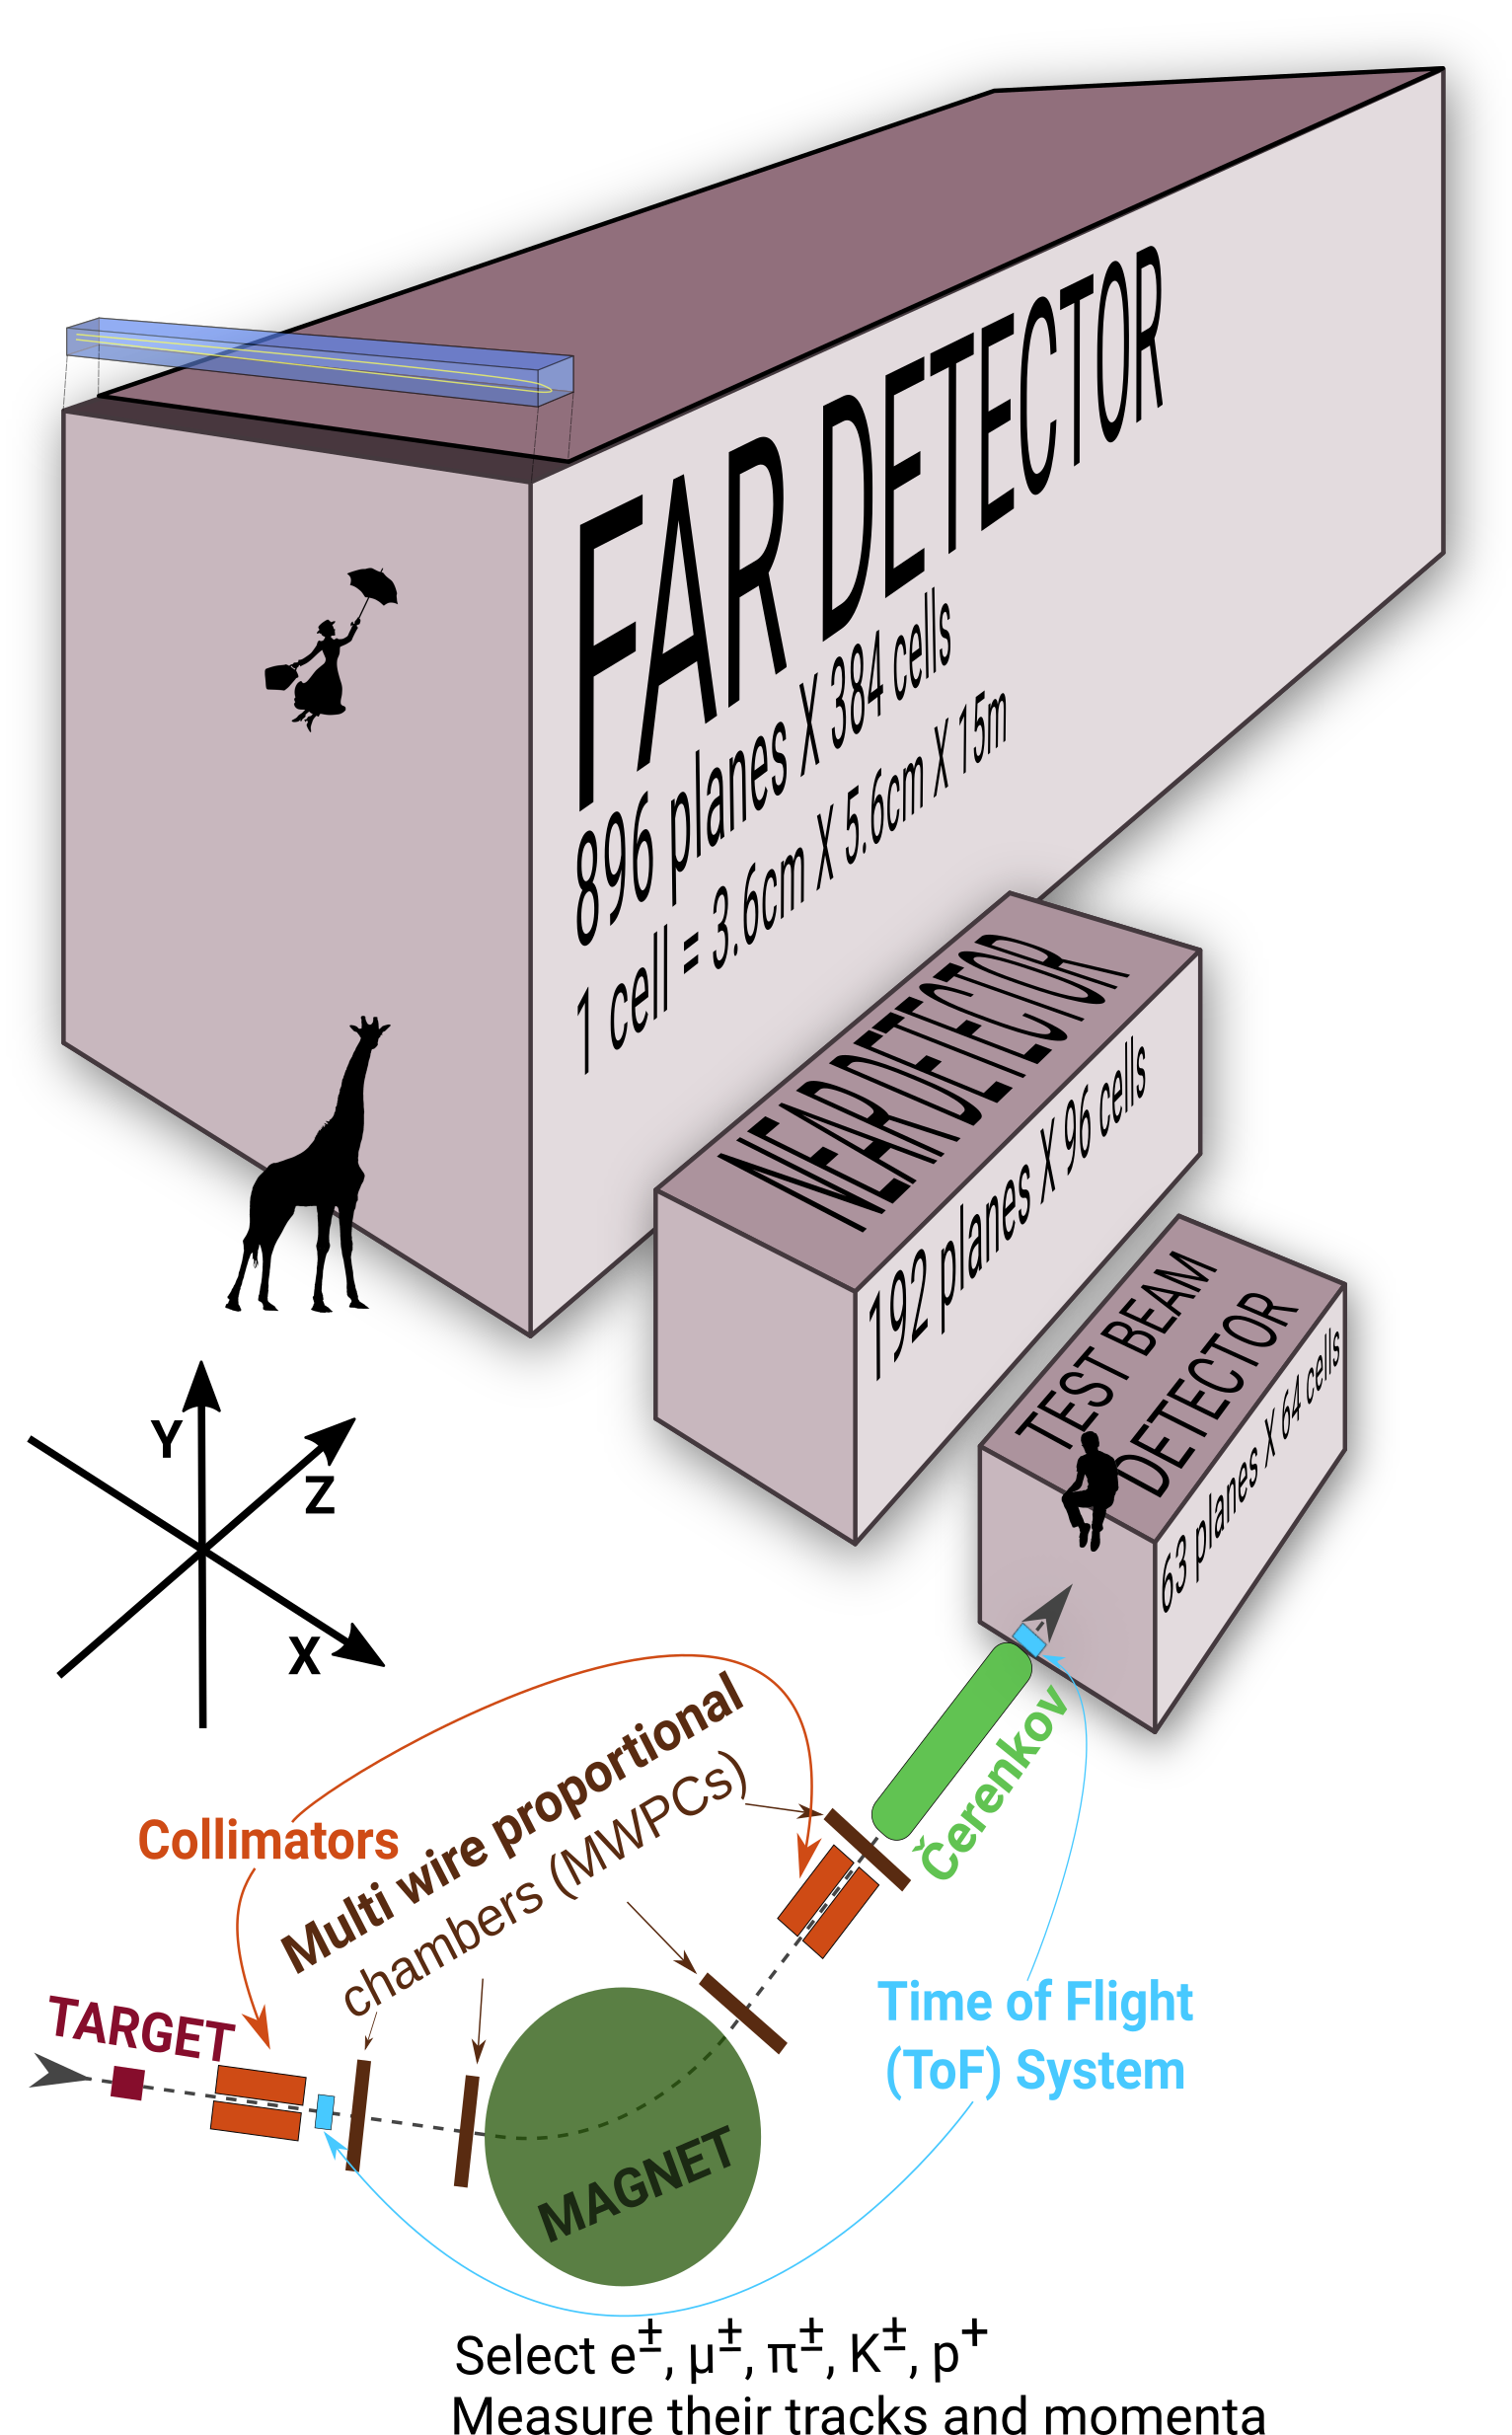
\includegraphics[width=.7\textwidth]{Plots/TBCalibration/TestBeamDetectorWithArrows.png}
\caption[Comparison of Test Beam detector to the Near and Far Detectors]{Comparison of Test Beam detector scale to the \acrshort{NOvA} \acrshort{ND} and \acrshort{FD} (and a man, giraffe, or Mary Poppins). Also shown are the Test Beam beamline detectors and components (not to scale), with arrows showing the direction of the beam. An example of a detector cell with \acrshort{WLS} fibre looped inside it is also shown (not to scale). The three black arrows show the orientation of the detector coordinate system.}
\label{fig:TBDetector}
\end{figure}

%Should I aslo talk about the beam halo? Could that have an influence on the calibration? Maybe it's the peaks in the cosz distribution?

The operation of the Test Beam detector started with commissioning runs in June 2019 and ran, with an exception of regular summer shutdowns, until July 2022, after which it was decommissioned. The Test Beam data taking is divided into \textit{periods}, which are defined in Tab.~\ref{tab:TestBeamPeriods}. Period 1 only lasted for about a month and with only a half-filled detector, as explained below. It was therefore only used for detector commissioning and will not be used in any of the Test Beam physics analysis, or in the calibration.
\begin{table}[!ht]
\centering
\caption{Test Beam detector data taking periods.}
\def\arraystretch{1.4}
\begin{tabular}{l@{\hskip 1in}lcl}
Period 1 & June $3^{\textsf{rd}}$ 2019 & - & July $6^{\textsf{th}}$ 2019\\
Period 2 & December $5^{\textsf{th}}$ 2019 & - & March $20^{\textsf{th}}$ 2020\\
Period 3 & January $12^{\textsf{th}}$ 2021 & - & June $27^{\textsf{th}}$ 2021\\
Period 4 & November $30^{\textsf{th}}$ 2021 & - & July $10^{\textsf{th}}$ 2022
\end{tabular}
\label{tab:TestBeamPeriods}
\end{table}

Majority of the Test Beam detector and its instrumentation is identical to the other \gls{NOvA} detectors, with a few exceptions that could have an impact on the calibration. We are going to identify and discuss these differences in this section.

%[docdb:15750 - NOvA Test Beam task force report]: The test beam program was included in the NOvA proposal [1] and was considered as an essential part of the experiment since its inception. The main tangible result of these initial plans and later discussions was a production of special small extrusion modules, made at the end of the modules production stage, as possible components of a future test beam detector. In fact, this production followed and was based on initial simulations of a possible test beam experiment [5].

\subsubsection*{Beamline}
The beam for the Test Beam experiment originates from the same $\unit[120]{GeV}$ Main Injector protons used in \gls{NuMI}, extracted once a minute in a continuous $\unit[4.2]{s}$ spill~\cite{NOvATestBeamWallbangProceedings2020.pdf}. The protons are impinged on a copper target producing mostly protons and pions, which are then directed towards a second target, producing the tertiary beam of particles used in the Test Beam detector. As can be seen in Fig.~\ref{fig:TBDetector}, two collimators are used to direct the tertiary beam and a magnet to select the desired momentum. Particle tracking is done using the four \glspl{MWPC} and particle identification is done with a combination of \gls{ToF} detectors and a Cherenkov detector set for electron detection.

\subsubsection*{Detector parameters}
The \gls{NOvA} Test Beam detector consists of two 31-plane blocks, each beginning and ending with a vertical plane, with an additional horizontal plane glued in-between them to preserve the alternating pattern \cite{NOvA-doc-29543}. Each plane consists of 2 modules side-by-side, both made up of 32 cells. Each cell is $2.6\,\unit{m}$ long with an inner (without the PVC) depth and width of $5.9\,\unit{cm}$ and $3.8\,\unit{cm}$ respectively, same as for the other \gls{NOvA} detectors. This brings the final dimensions of the Test Beam detector to 63 planes $\times$ 64 cells, or $2.6\times 2.6\times 4.1\,\unit{m^3}$.

The 63 planes are numbered from 0 to 62, with even numbers corresponding to vertical planes and odd numbers to horizontal planes. Cells are numbered 0 to 63, going from bottom to top for horizontal planes and left to right, when facing the front of the detector, for vertical planes.

The detector coordinate system is illustrated in Fig.~\ref{fig:TBDetector}. It is centred with $\left(0,0,0\right)$ in the centre of the first plane \cite{NOvA-doc-58388}. The x axis runs left to right when facing the front of the detector, y axis from bottom to top, and z axis goes along the beam direction from front to the back of the detector. Position within each cell ($w$) is aligned with the x (y) axis for the horizontal (vertical) cells, with $w=0$ centred in the middle of each cell. The exact geometry of the Test Beam detector was measured in several alignment surveys and is saved in gdml files \cite{NOvA-doc-57955}.

In the past we encountered an issue when trying to align the Test Beam detector with the beamline measurements by rotating the detector. This broke several assumptions within the Test Beam geometry \cite{NOvA-doc-58388} and manifested as uncalibrated cells in the back of the detector \cite{NOvA-doc-57516}. This was fixed by realigning both the detector and the beamline separately, based on the last alignment survey, measured during the decommissioning of the detector.

%FD: maxPlane=900, maxCell=390. ND: maxPlane=220, maxCell=100. TB: maxPlane=63, maxCell=64

\subsubsection*{Scintillator}
%[TB task force report]: The NDOS decommissioning yielded 25000 gallons of scintillator. Since storage available is limited to 12000 gallons, it was decided to blend most of the 5000 gallons of existing ND/FD scintillator with the NDOS scintillator. 200 gallons of ND/FD scintillator, which has a slightly higher photon yield, are reserved for special studies. We also plan to reuse the NDOS secondary containment tub to provide oil+scintillator containment in case the test beam detector undergoes a catastrophic structural failure.

Test Beam used a combination of the leftover \gls{ND} and \gls
{FD} production scintillator oils and the oil drained from the \gls{NOvA} \gls{NDOS} test detector. The used scintillator oils also differ in the way they were stored since the \gls{ND} and \gls{FD} filling, or the \gls{NDOS} draining, which apparently impacted its quality. These factors have a significant effect on the energy deposition within them. The distribution of individual scintillator oils and the relative difference in their energy response can be seen in Fig.~\ref{fig:Scintillators}.

%The Test Beam detector is filled with several different versions of the NOvA scintillator oil, which differ mainly in the way they were stored since the filling of the near and far detectors. This is illustrated on figure \ref{figScintillators}.

\begin{figure}[!ht]
\centering
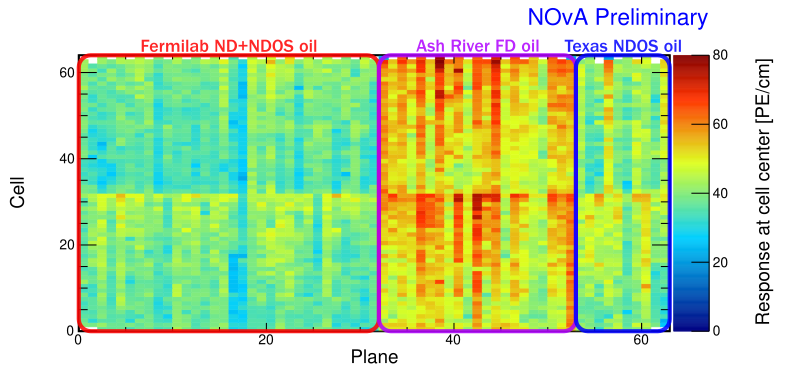
\includegraphics[width=\textwidth]{Plots/TBCalibration/TestBeamScintillatorOils.png}
\caption[Scintillator oils used in the Test Beam detector]{Uncorrected energy response in the centre of cells across the Test Beam detector showing a clear distinction between different scintillator oils, labelled with coloured boxes and descriptions.}
\label{fig:Scintillators}
\end{figure}

There are four distinct samples of \gls{NOvA} scintillator oil used in the Test Beam detector:
\begin{enumerate}
\item Mixed \gls{ND} production oil and \gls{NDOS}-drained oil stored in a tanker and four tanks outside in \gls{Fermilab} \cite{NOvA-doc-38349};
\item Separate \gls{ND} production oil and \gls{NDOS}-drained oil stored underground in barells at the MiniBooNE\footnote{MiniBooNE~\cite{MiniBooNEWebsite} is a \gls{Fermilab} experiment located close to the \gls{NOvA} \gls{ND}} cavern \cite{NOvA-doc-33012};
\item \gls{FD} production oil stored inside in Ash River in `totes' under several layers of black plastic \cite{NOvA-doc-34067};
\item \gls{NDOS}-drained oil stored mainly inside at Texas A\&M University and University of Texas at Austin \cite{NOvA-doc-38740, NOvA-doc-39088}.
\end{enumerate}

%The original plan \cite{NOVA-doc-34196} was to use the tanker and tank scinitillator for the entire Test Beam detector. However, due to extreme cloudeness of the scintillaotr in the tanks 

The original plan \cite{NOvA-doc-34196} was to only use the tanker/tank scintillator (sample \#1). First tests showed acceptable results and the tanker oil was used to fill out almost the entirety of the first block of the detector (first 32 planes) \cite{NOvA-doc-38349}. However, when the oil from tank \#2 was loaded into the tanker, it became extremely cloudy and unusable, possibly due to contamination with water accumulated at the bottom of the tanks. The rest of the first block was therefore topped up with high quality scintillator from \gls{NDOS} (sample \#2). This is labelled as `\gls{Fermilab} \gls{ND}+\gls{NDOS} oil' in Fig.~\ref{fig:Scintillators}.

%NDOS+ND scin3llator were stored in MEast tank farm in translucent tanks open to the atmosphere in 2016 [docdb:41229]
%docdb:41229 actually contains a pretty good description of the whole story

%First Tanker (2730 gallons pumped) used to fill 97.5% of first block ... Missing ~2.5 gallon top-off... Decided to use reserved NDOS 55-gallon drums... Used 65 gallons for detector, 11 gallons to clean up fill lines

%Even before the extreme cloudiness was discovered, it was known that the oil from the tanks has lost much of its original light yield properties. Reasons vary from water contamination to insects and dirt contamination \cite{NOVA-doc-34046-v2}. Yet it was still decided to use the tank 2 oil \cite{NOVA-doc-34196}. It was also decided not to mix the various oils (tanker/tank/NDOS/Ash River) as studying energy deposition in different types of oils could lead to some interesting insights \cite{NOVA-doc-34046-v2}.

%"One of the promising studies we see coming out of this is to understand the differences in performance for different type of energy depositions of scintillator A vs B vs C. " [docdb:34046]

The first 21 planes of the second block (planes 32 to 52) were filled with the \gls{FD} production scintillator shipped in from Ash River (sample \#3) \cite{NOvA-doc-41961}. These planes were again topped up with the \gls{ND}+\gls{NDOS} scintillator (sample \#2).

The last 10 planes (planes 53 to 62) \cite{NOvA-doc-41961} were filled with the `Texas' scintillator (sample \#4), which has higher light yield than the one from the tanker, but lower than the Ash River one \cite{NOvA-doc-38740}.

%[docdb:38349] 2730 gallons of scintillator transferred to detector from the tanker. On April 16, circulated 20 gallons from tanker, and took scintillator sample. Extreme cloudiness meant 0\% light transmission (>=95\% required). Strongly suspect problem due to water accumulated at the bofom of tankers vented to the atmosphere since 2016, mixed with oil by pump. Used 2/4 reserved NDOS 55-gallon drums for top-off...  completed top-off of all Block 0 modules

In total, the Test Beam detector is filled with 5418 gallons of scintillator oil with a weight of approximately 28.6 tons \cite{NOvA-doc-29543}.

\subsubsection*{Readout}
The Test Beam detector uses in total 126 \glspl{FEB}, each reading out signal from 32 cells \cite{NOvA-doc-29543}. The readout is located on the top and right side (when looking at the front) of the detector. 118 \glspl{FEB} are version 4.1, same as in the \gls{FD}, and 8 \glspl{FEB}, located in pairs on planes 16, 17, 48 and 49, are version 5.2, same as in the \gls{ND}. As was described in Sec.~\ref{sec:DAQ}, the \gls{ND} \glspl{FEB} are designed to read out data at a faster rate than the \gls{FD} \glspl{FEB} and using a mix of \gls{FEB} types allows us to study the difference in their response and to validate both versions in the same environment~\cite{LackeyThesisNOvATBProtons2022.pdf}.

%The Near and Far Detectors use different front-end electronics since they handle different data volumes; the Test Beam Detector is instrumented with both types to facilitate a complete characterization of both NOvA neutrino detectors. [NOvATestBeam.pdf - Mike's proceedings]

\subsubsection*{Environment}
The enclosure that housed the Test Beam detector was made up of a concrete platform covered by a metal semi-cylindrical roof. Therefore, unlike the \gls{ND} and \gls{FD}, the Test Beam detector did not have any overburden to shield it from cosmic particles, affecting their rate and energies inside the detector. The temperature and humidity were controlled by a humidity, ventilation and air conditioning control system and monitored by a range of sensors. The temperature was kept to around $\unit[20]{^{\circ}C}$ and within the range of $\unit[18-22]{^{\circ}C}$, except for about three months in the beginning of Period 3 data taking, when it was kept to within $\unit[16-20]{^{\circ}C}$.

%Is the HVAC the only systema that is controling the environment at MC7b?

%From docdb:29543
%Temperature very stable during winter months (heaCng is installed at MC7). However, dew point went over 10C ND shutdown threshold several times.
%Alex'es summary in docdb:30750:
%Ordered HVAC unit with electric reheat and dewpoint control, in essence over-cooling to maintain dewpoint then reheat to maintain temperature.

%Can I describe what is the shielding in MC7b? What is the white stuff from? It's basically the only thing shielding the detector from the cosmics and temperatures. Also need to say there is an HVAC system

%Placed in the Fermilab Test Beam Facility with no overburden. Describe environmental controls, temperature dependence etc. Maybe add plots from environmental control (temperature differences etc.) with descriptions of where were the readings taken.

\subsubsection*{Underfilled cells issue}
The Test Beam detector is slightly tilted around the z axis by about $0.7^{\circ}$ towards the readout (top of the detector is tilted right when facing the front of the detector). This caused the top cells of both modules of all the horizontal planes (cells 31 and 63) to be underfilled, creating an air bubble on the left side of the detector and severely affecting the energy response in those cells \cite{LackeyThesisNOvATBProtons2022.pdf}. This was fixed \cite{NOvA-doc-49439} during the period 3 running by adding extensions to the filling ports and overfilling the horizontal cells with the \gls{ND}+\gls{NDOS} scintillator (sample \#2 from the scintillator description). More details on this issue and its effects and on how it was handled in calibration are detailed in Sec.~\ref{sec:TBCalibration_period3}.
%This scintillator was also used in the first half of the detector (Fermilab ND+NDOS oil on figure \ref{figScintillators}), but is different from the "Ash River oil" used in part of the second half of the detector (bright part of figure \ref{figScintillators}). The overfilling was done in April 2021 in 3 stages in between the full operation of the Test Beam detector.

%The detector is tilted around z axis towards the readout by about 0.7 degrees (the largest tilt is for the 11th plane of 0.79330 degrees. The ND has an oposite tilt of -0.2515 degrees on average (but also the readout is on the opposite side, so is it actually the same tilt?). Correcting this by 8 degrees would require lifting the east edge by at least 3.66cm, or to correct it to the ND tilt by lifting the east edge by 4.17cm. [docdb:47491 - this is the original talk by Teresa explaining the tilt on 21st Sep 2020]

%Also need to mention that the detector was then overfilled [docdb:49439 or 49827] but with a scintillator from the NDOS drums, causing the discrepancy between the high quality Ash River scintillator and the NDOS scintillator. But need to mention this after the scintillator part.
%The overfilling was done in three stages:
%\begin{enumerate}
%\item Overfilling the back 9 horizontal and the 7th horizontal from the front by April 21st
%\item Overfilling of the 15 front cells (except the 7th, which was already done, and the 14th, %with problems drilling vent hole) by April 27th
%\item Overfilling of the remaining 8 horizontals by April 30th
%\end{enumerate}

%From Teresa's thesis:
%The pitch and yaw of the detector was 2.464◦ around x and 0.487◦ around z. Roll (around beam direction) of each plane. Unfortunately, the direction of the roll means the east side of the detector is slightly lower than the west side. The east side is where the readout and fill ports for the scintillator are. As a result, the top cell in each horizontal module is underfilled, with an air bubble on the west side.
